%%%%%%%%%%%%%%%%%%%%%%%%%%%%%
% Sorry, I don't know how to do it better...
%%%%%%%%%%%%%%%%%%%%%%%%%%%%%
\newcommand\parttres{%
  \cleardoublepage
  \thispagestyle{plain}%
  \null\vfil
   \secdef\kkpart\kkpart}
\def\kkpart[#1]#2{%
      \relax
      \refstepcounter{part}%
      \addcontentsline{toc}{part}{\thepart\hspace{1em}#1}%
    {\centering
     \interlinepenalty
     \normalfont
      \relax
       \huge\bfseries \partname\nobreakspace\thepart
       \par
       \vskip 20pt
     \Huge \bfseries #2\par}%
    \kkendpart}
\def\kkendpart{
\vspace*{3cm}
\begin{center}
\begin{minipage}{0.8\textwidth}
\textbf{ \noindent En aquesta part del llibre aprendreu a definir els vostres propis mètodes. Això us permetrà reutilitzar
seqüències de missatges, i sereu capaços de definir mètodes complexos a partir de mètodes més 
senzills.}
\end{minipage}
\end{center}
	\vfil\newpage
                \null
                \thispagestyle{empty}}
%%%%%%%%%%%%%%%%%%%%%%%%%%%%%
%%%%%%%%%%%%%%%%%%%%%%%%%%%%%
%%%%%%%%%%%%%%%%%%%%%%%%%%%%%

\parttres{Posar en joc l'abstracció}

\chapter{Mètodes: seqüències de missatges amb nom}
\label{cap12}

Fins ara, heu estat utilitzant \emph{scripts} per crear robots i enviar-los seqüències de missatges. Utilitzar \emph{scripts} té l'avantatge de ser l'aproximació més immediata, però té limitacions importants. Una de les principals és que un \emph{script} no pot ser invocat per un altre \emph{script}. Aquest és un problema seriós, ja que un \emph{script} no pot ser reutilitzat per altres \emph{scripts}. Heu de reescriure la mateixa seqüència de missatges una vegada i una altra.

No estaria bé que poguéssim definir una mena d'\emph{script} la seqüència de missatges del qual pogués ser enviada a qualsevol robot? De fet, això és possible i aquestes seqüències d'\emph{scripts} es diuen \emph{mètodes} (en el context d'aquest llibre no entrarem a estudiar tota la potència que poden proporcionar els mètodes, ja que això ens introduiria de ple en el complicat món de la programació orientada a objectes). Un \emph{mètode} és un \emph{script} amb nom. El nom del mètode pot utilitzar-se en un \emph{script}, o fins i tot en un altre mètode, per invocar el mètode. Si us fixeu, no hi ha gairebé res de nou en això: tots els missatges per a robots que heu utilitzat fins ara representen mètodes que podeu fer servir amb qualsevol robot!

En aquest capítol aprendreu com definir mètodes. Ja sabeu gairebé tot el que cal saber per escriure un mètode. Tot i així, un mètode s'ha de definir amb un editor especial anomenat \emph{explorador (o navegador) de codi}. Començarem comparant un \emph{script} i un mètode. Després definirem un mètode, i finalment, entrarem en detall a veure què hem aconseguit.

\section{\emph{Scripts} versus mètodes}
\index{scripts@\emph{scripts}!versus mètodes|(}
\index{dibuixar!quadrats|(}
\index{metodes@mètodes!versus \emph{scripts}|(}
Anem a retrobar un dels \emph{scripts} que ja heu escrit, per exemple l'\emph{Script}~\ref{scr12-1}, que crea un robot i li diu com dibuixar un quadrat amb costat de mida 100 píxels.\index{quadrats!dibuixar|(}
\begin{script}  Pica dibuixa un quadrat senzill.
\textsf{\upshape
\begin{tabbing}
\hspace{5mm} \= \kill
$|$ pica $|$\\
pica := Bot nou.\\
4 vegadesRepetir:\\
\> [  pica giraEsquerra: 90.\\
\> pica ves: 100  ]\\
\end{tabbing}
}
\label{scr12-1}
\end{script}

El problema amb aquest \emph{script} és que cada cop que necessiteu dibuixar un quadrat de costat 100 píxels heu de \emph{copiar} les darreres tres línies de l'\emph{Script}~\ref{scr12-1}. És més, si voleu que un altre robot (per exemple, \textsf{daly}) dibuixi el quadrat, heu de canviar el nom \textsf{pica} a \textsf{daly} a tot arreu. Això ho podeu veure a l'\emph{Script}~\ref{scr12-2}.
\begin{script}  Pica i daly dibuixen cadascú un quadrat senzill.
\textsf{\upshape
\begin{tabbing}
\hspace{5mm} \= \kill
$|$ pica daly $|$\\
pica := Bot nou.\\
daly := Bot nou.\\
daly salta: 200.\\
daly color: Color vermell.\\
\\
{\bfseries 4 vegadesRepetir:}\\
\> {\bfseries [  pica giraEsquerra: 90.}\\
\> {\bfseries pica ves: 100  ].}\\
{\bfseries 4 vegadesRepetir:}\\
\> {\bfseries [  daly giraEsquerra: 90.}\\
\> {\bfseries daly ves: 100  ].}\\
\end{tabbing}
}
\label{scr12-2}
\end{script}

Per aquestes raons, treballar amb \emph{scripts} no és fàcil. De fet, sospitem que les tres afirmacions següents reflecteixen part de la vostra experiència personal amb els \emph{scripts}:
\begin{itemize}
\item Escriure \emph{scripts} llargs és una tasca penosa.
\item Repetir \emph{scripts} llargs és avorrit i susceptible d'introduir errors.
\item Quan un copia \emph{scripts} complexos, la probabilitat de cometre un error de programació, com ometre una línia, és alta (un error de programació és un error dins la lògica del programa. Per contrast amb els errors de sintaxi, que són trobats ràpidament per l'ordinador ja que són errors en l'estructura del programa, els errors de programació poden ser bastant difícils de trobar).
\end{itemize}

Per superar aquestes dificultats, ens agradaria \emph{definir} una seqüència de missatges una vegada, donar-li un \emph{nom}, i després poder \emph{enviar la seqüència amb nom} com un sol missatge a qualsevol robot, tal i com hem fet enviant missatges predefinits com \textsf{ves:}, \textsf{nord} o \textsf{salta:}.

D'aquesta manera, podríem definir un \emph{mètode} nou, anomenat \textsf{quadrat}, i aleshores escriure l'\emph{Script}~\ref{scr12-3}. No executeu l'\emph{script} de moment, perquè el mètode \textsf{quadrat} encara no ha estat definit. Un cop tingueu el mètode \textsf{quadrat}, ja no us caldrà copiar ni adaptar la seqüència de missatges definint un quadrat. Senzillament podeu utilitzar-la dues vegades. L'enviament de missatge \textsf{pica quadrat} li dirà a \textsf{pica} que dugui a terme les instruccions codificades dins el mètode \textsf{quadrat}.

Esperem haver-vos convençut que aprendre a definir mètodes valdrà la pena.
\begin{script}  Pica i daly dibuixen quadrats utilitzant el mètode \textsf{{\upshape quadrat}}.\index{scripts@\emph{scripts}!versus mètodes|)} \index{quadrats!dibuixar|)}
\textsf{\upshape
\begin{tabbing}
\hspace{5mm} \= \kill
$|$ pica daly $|$\\
pica := Bot nou.\\
daly := Bot nou.\\
daly salta: 200.\\
daly color: Color vermell.\\
{\bfseries pica quadrat.}\\
{\bfseries daly quadrat.}\\
\end{tabbing}
}
\label{scr12-3}
\end{script}

\section{Com definir un mètode?}
\index{dibuixar!quadrats|)}
\index{metodes@mètodes!versus \emph{scripts}|)}
\index{Explorador de la classe Bot!propietats de}
En aquesta secció us donarem una recepta per crear mètodes. A Squeak podeu definir mètodes en qualsevol objecte, en aquest llibre, però, definireu mètodes només pels robots. Per ajudar-vos, hem desenvolupat un explorador de codi anomenat \textsf{Explorador de la classe Bot}, només per definir mètodes pels vostres robots. Podeu aconseguir un \textsf{Explorador de la classe Bot} arrossegant la seva icona des de la solapa blau fosc o via el menu \textbf{obre\dots} i després triant \textbf{explorador Bots}.

Utilitzar un \textsf{Explorador de la classe Bot} per definir un mètode requereix que (1) trieu o creeu una categoria nova de mètodes, que és una mena de carpeta de mètodes; (2) escriviu el mètode; i (3) el compileu. Descriurem aquests passos en les properes seccions. Primer, deixeu-nos explorar amb detall les diferents parts de l'\textsf{Explorador de la classe Bot}.

\subsection{\textsf{Explorador de la classe Bot}}
\index{Explorador de la classe Bot!utilitzar el}
Definir mètodes requereix una nova eina: l'editor mostrat a la figura~\ref{fig1201}. Aquest explorador és una versió simplificada de l'explorador que utilitzen els programadors en Smalltalk. L'explorador consisteix en tres parts, o \emph{subfinestres}.\index{subfinestres de l'Explorador de la Classe Bot, explicació de}
\begin{figure}[h!]
\begin{center}
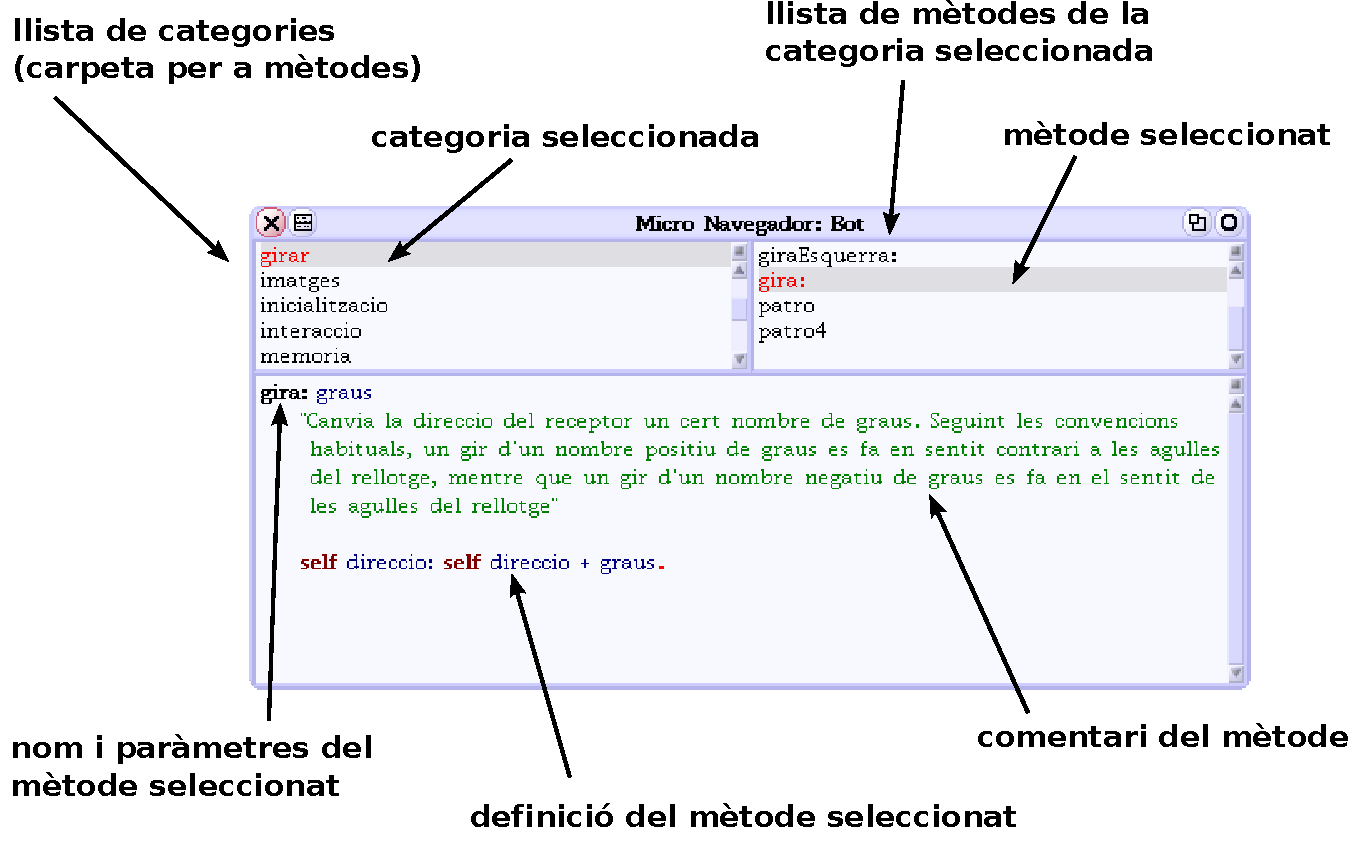
\includegraphics[scale=0.55]{Imatges/figura12-1.pdf}
\end{center}
\caption{Un \textsf{\upshape Explorador de la classe Bot} mostrant la definició (subfinestra inferior) del mètode \textsf{\upshape gira:} (seleccionat a la subfinestra superior dreta) pertanyent a la categoria \textsf{\upshape girar} (seleccionada a la subfinestra superior esquerra).}
\label{fig1201}
\end{figure}
\begin{itemize}
\item[] \textbf{Categories.} La subfinestra superior esquerra conté la \emph{llista de categories}. Mostra les diferentes categories de mètodes. Les categories de mètodes són només noms per a grups de mètodes que ajuntem per trobar més de pressa la informació. A la figura~\ref{fig1201}, la categoria \textsf{girar} s'ha seleccionat; agrupa totes les operacions que tenen a veure amb els canvis de direcció dels robots. Podeu veure també altres categories que agrupen altres mètodes per als robots. 
\item[] \textbf{Mètodes.} La subfinestra superior dreta conté la \emph{llista de mètodes}. Aquesta llista mostra els noms dels mètodes dins la categoria seleccionada. A la figura~\ref{fig1201}, veiem llistats cinc mètodes \textsf{apuntaA:}, \textsf{giraA:}, \textsf{giraDreta:}, \textsf{giraEsquerra:} i \textsf{gira:}. El mètode \textsf{gira:} està seleccionat.\index{metodes@mètodes!definir amb l'Explorador de la classe Bot}
\item[] \textbf{Definició de Mètodes.} La subfinestra inferior conté l'\emph{editor de codi}. Mostra la definició del mètode el nom del qual està seleccionat, juntament amb un comentari opcional. Aquesta subfinestra és també el lloc on podeu escriure el codi d'un mètode nou.
\end{itemize}

\subsection{Crear una nova categoria de mètodes}
\index{categories!crear pels mètodes|(}
\index{metodes, categories@mètodes, categories de|(}
Agrupem els mètodes per categories. Una categoria es defineix donant-li un nom. Per definir un mètode, o bé definim una categoria nova pel mètode o bé seleccionem una categoria ja existent. Crearem una nova categoria de nom \textsf{polígons regulars}. Aquí teniu els detalls:

\begin{itemize}
\item[\textbf{1.}] Feu clic amb el botó dret del ratolí (\emph{Alt}-clic o bé \emph{Option}-clic) a la llista de categories. Apareixerà un menú com el de la figura~\ref{fig1202}.
\begin{figure}[h]
\begin{center}
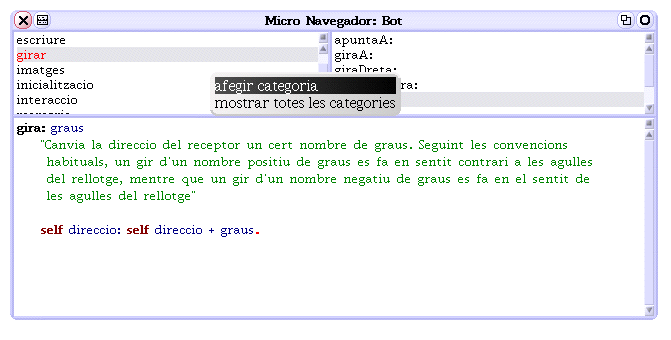
\includegraphics[scale=1.75]{Imatges/figura12-2.png}
\end{center}
\caption{Per crear una nova categoria de mètodes, obriu el menú de categories i seleccioneu \textsf{\upshape afegir categoria}.}
\label{fig1202}
\end{figure}
\item[\textbf{2.}] Seleccioneu l'opció \textsf{afegir categoria} d'aquest menú.
\item[\textbf{3.}] Escriviu el nom de la categoria al quadre de diàleg que apareixerà tot seguit, com podeu veure a la figura~\ref{fig1203}. Podeu triar qualsevol nom per a la categoria. Naturalment, noms significatius són millors que noms que no ho són quan voleu compartir la vostra feina amb altra gent o trobar el vostre mètode hores, dies o mesos més tard.
\begin{figure}[h]
\begin{center}
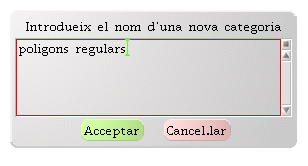
\includegraphics[scale=2.5]{Imatges/figura12-3.png}
\end{center}
\caption{Escriviu un nou nom de categoria al quadre de diàleg i feu clic al botó \textsf{\upshape Acceptar}.}
\label{fig1203}
\end{figure}
\item[\textbf{4.}] Feu clic al botó \textsf{Acceptar} per validar la vostra tria.
\end{itemize}

Com veieu a la figura~\ref{fig1204}, el nom de la nova categoria apareix a la subfinestra de categories i està seleccionat automàticament. L'editor està preparat per acceptar una nova definició de mètode. Us mostra un recordatori de com cal definir un mètode, que haureu d'eliminar quan comenceu a escriure el vostre mètode. Ara ja esteu preparats per definir el vostre primer mètode.\index{categories!crear pels mètodes|)} \index{metodes, categories@mètodes, categories de|)}
\begin{figure}[h]
\begin{center}
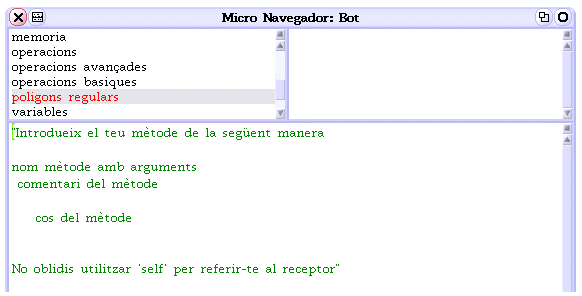
\includegraphics[scale=2]{Imatges/figura12-4.png}
\end{center}
\caption{La nova categoria està preparada.}
\label{fig1204}
\end{figure}

\newpage

\subsection{Definir el vostre primer mètode}
\index{metodes@mètodes!definir amb l'Explorador de la classe Bot|(}
Si la categoria on voleu afegir el vostre mètode no està seleccionada, seleccioneu-la. Aleshores escriviu el contingut del Mètode~\ref{met12-1} (després d'aquest paràgraf) dins la subfinestra de l'editor de codi. Per fer això, seleccioneu tot el text dins l'editor de codi i comenceu a escriure el mètode.
\newtheorem{metode}{Mètode}[chapter]
\begin{metode} Un nou mètode per dibuixar un quadrat amb costats de mida 100 píxels.
\noindent
\textsf{\upshape
\begin{tabbing}
\hspace{5mm} \= \hspace{10mm} \= \kill
{\bfseries quadrat}\\
\> {\itshape ``Dibuixa un quadrat amb costats de mida 100 píxels''}\\
\\
\> 4 vegadesRepetir:\\
\>\> [  self ves: 100.\\
\>\> self giraEsquerra: 90  ]\\
\end{tabbing}
}
\label{met12-1}
\end{metode}

Definir un mètode és un procés en tres passos:
\begin{itemize}
\item[\textbf{1.}] \textbf{Escriure el mètode.} Escriure codi dins l'editor de codi funciona exactament igual que amb l'editor d'\emph{scripts}. Primer elimineu el text que hi hagi a la subfinestra de l'editor de codi. La manera més senzilla de fer això és apuntar el ratolí al començament de la subfinestra de l'editor i fer clic abans del primer caràcter. Això seleccionarà tot el text de l'editor de codi. Un cop acabeu d'escriure el nou mètode, el codi dins la subfinestra de l'editor de codi hauria de semblar el que teniu a la figura~\ref{fig1205}.
\begin{figure}[h!]
\begin{center}
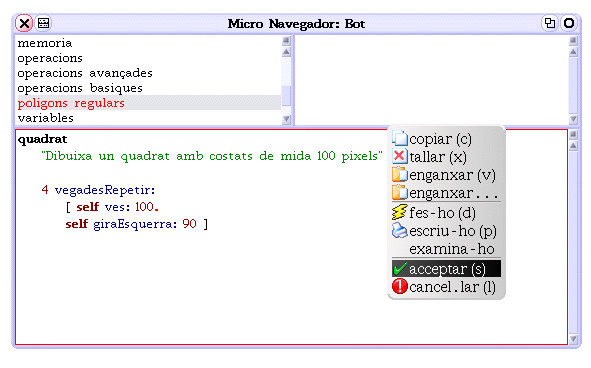
\includegraphics[scale=1.5]{Imatges/figura12-5.png}
\end{center}
\caption{Després d'escriure el mètode \textsf{\upshape quadrat}, l'heu de compilar utilitzant el menú de l'editor de codi.}
\label{fig1205}
\end{figure}
\item[\textbf{2.}] \textbf{Compilar el mètode.}  Feu clic per fer aparèixer el menú de l'editor de codi, com veieu a la figura, i seleccioneu l'opció \textbf{acceptar}. En fer això la definició del vostre mètode es \emph{compilarà}, és a dir, serà transformada a una representació que l'ordinador pugui entendre i executar. Un mètode nou anomenat \textsf{quadrat} ara apareix a la llista de mètodes. Si haguéssiu comès cap error mentre escrivíeu el mètode, Squeak es queixaria igual que ho feia amb els \emph{scripts}.
Si heu definit el mètode correctament, hauríeu de poder compilar el mètode sense que Squeak es queixés. L'explorador reflectirà el fet que la compilació és completa i que els robots ara poden entendre missatges que continguin el nou mètode mostrant el nom del nou mètode a la llista de mètodes (figura~\ref{fig1206}).\index{metodes@mètodes!compilar i comprovar}
\item[\textbf{3.}] \textbf{Comprovar el mètode.} Segons la dita, la manera de comprovar si un pastís està ben fet és tastant-lo. Aquí igual, no heu acabat de crear el vostre mètode nou fins que l'heu comprovat, ja que el mètode que heu definit pot no fer el que teníeu al cap. Ara ja podeu executar l'\emph{Script}~\ref{scr12-3}. Hauríeu d'obtenir un quadrat negre i un altre de vermell.
\end{itemize}

Observeu que un mètode pot utilitzar-se molts cops, com queda demostrat a l'\emph{Script}~\ref{scr12-3}. Això ja ho sabíem. De fet, ho hem utilitzat des que vam començar el llibre: selectors de missatge com \textsf{ves:} o \textsf{giraEsquerra:} són els noms de mètodes definits de la mateixa manera que el mètode \textsf{quadrat}.\index{metodes@mètodes!definir amb l'Explorador de la classe Bot|)}\index{metodes@mètodes!utilitzar i reutilitzar}

\section{Què hi ha en un mètode?}
\index{metodes@mètodes!components de|(}
Us hem demanat que escriviu un mètode sense gaire explicacions. Ara és el moment d'analitzar l'estructura d'un mètode.

Un mètode està compost d'un \emph{nom}, un \emph{comentari} opcional i el \emph{cos del mètode} (una seqüència d'expressions), com es veu a la figura~\ref{fig1206}. El nom del mètode també pot contenir paràmetres (veure capítol~\ref{cap14}) i el cos del mètode pot també definir variables locals utilitzant les barres verticals \textbar \hspace{2mm} \textbar .
\begin{figure}[h]
\begin{center}
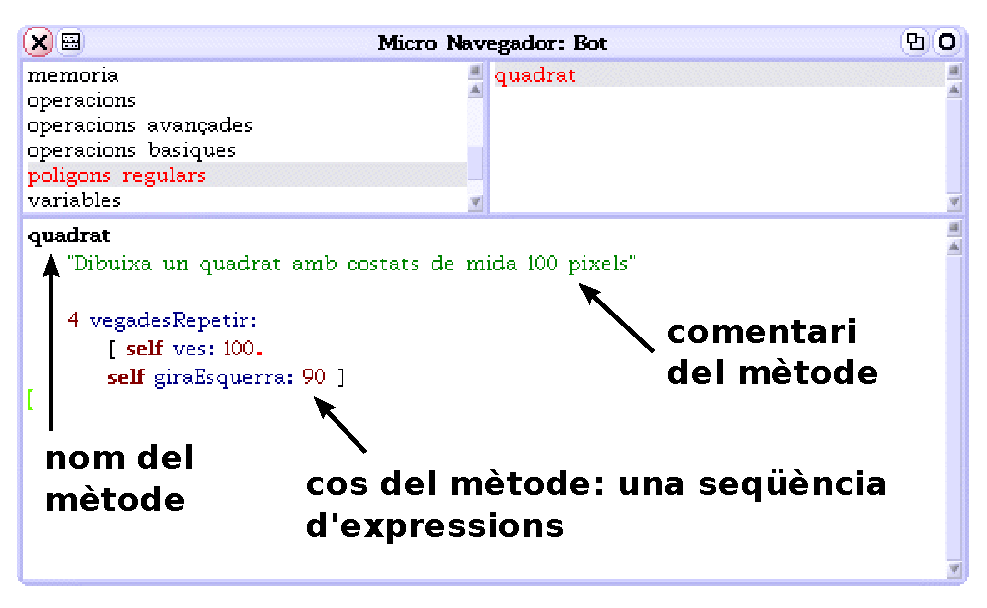
\includegraphics[scale=0.5]{Imatges/figura12-6.pdf}
\end{center}
\caption{Un mètode està format per un nom, un comentari opcional i el cos del mètode.}
\label{fig1206}
\end{figure}

\begin{itemize}
\item[] \textbf{Nom del mètode.} El nom d'un mètode hauria de representar el que fa el mètode, no com ho fa. Quan voleu que algú obri una porta, oi que no li expliqueu tota la física i les matemàtiques que hi ha relacionades? Doncs amb els mètodes és el mateix.

\noindent
\rule{142mm}{2pt}\\
\noindent
\textbf{Important!} El nom d'un mètode ha de representar sempre què fa el mètode, no com ho fa\\
\noindent
\rule{142mm}{2pt}

Els noms de mètodes sense paràmetres, com \textsf{quadrat}, segueixen la mateixa sintaxi que els noms de les variables. Estan compostos de caràcters alfanumèrics (lletres i dígits) i comencen amb un caràcter en minúscules. En el nostre cas, el nom del mètode és \textsf{quadrat}.
\item[] \textbf{Comentari del mètode.} Un comentari és un text entre cometes dobles (\textsf{``Això és un comentari''}). El text no pot contenir cometes dobles. El text pot ser tan llarg com vulgueu, fins i tot pot ocupar diverses línies. \index{comentaris, incloure dins dels mètodes}  \index{'' (cometes), utilitzades en comentaris}  \index{cometes (''), utilitzades en comentaris}

\noindent
En general un comentari explica el propòsit i l'efecte d'un mètode. Explica com podem utilitzar-lo, però no com fa la seva feina. Qui vulgui saber com funciona el mètode pot llegir-ne el cos.

\noindent
Si el nom del mètode és prou clar, el comentari es pot ometre. En el nostre cas, el comentari del mètode és \textsf{``Dibuixa un quadrat amb costats de mida 100 píxels''}.
\item[] \textbf{Cos del mètode.} Després del comentari ve la definició del mètode, que és la seqüència de missatges que s'executaran com a resposta al missatge. En el nostre cas, el cos del mètode és:
\noindent
\textsf{\upshape
\begin{tabbing}
\hspace{10mm} \= \kill
4 vegadesRepetir:\\
\> [  self ves: 100.\\
\> self giraEsquerra: 90  ]\\
\end{tabbing}}
\end{itemize}
\index{expressions!relació amb els mètodes}\index{metodes@mètodes!relació amb les expressions}

\noindent
\rule{\textwidth}{2pt}
\noindent
\textbf{Important!} Un mètode és una seqüència d'expressions amb nom. Es compon d'un nom, un comentari opcional i una seqüència d'expressions. Un cop s'ha definit un mètode per a robots, qualsevol robot pot executar-lo en resposta a un missatge amb el mateix nom.\\   
\noindent
\rule{\textwidth}{2pt}

\subsection{\emph{Scripts} versus mètodes: Anàlisi}
\index{scripts@\emph{scripts}!versus mètodes|(}
\index{metodes@mètodes!components de|)}
\index{metodes@mètodes!versus \emph{scripts}|(}
Comparem el Mètode~\ref{met12-2} amb l'\emph{Script}~\ref{scr12-4}. Podeu veure-hi tres diferències significatives: (1) La línia de l'\emph{script} que declara la variable \textsf{pica} no és al mètode; (2) la línia que crea el robot tampoc hi és; (3) a la resta del mètode, la variable \textsf{pica} ha estat substituïda per \textsf{self}.
\begin{script}  Pica dibuixa un quadrat senzill.
\textsf{\upshape
\begin{tabbing}
\hspace{5mm} \= \kill
{\bfseries $|$ pica $|$}\\
{\bfseries pica := Bot nou.}\\
4 vegadesRepetir:\\
\> [  pica giraEsquerra: 90.\\
\> pica ves: 100  ]\\
\end{tabbing}
}
\label{scr12-4}
\end{script}

\begin{metode} Instruccions perquè qualsevol robot dibuixi un quadrat senzill.
\noindent
\textsf{\upshape
\begin{tabbing}
\hspace{5mm} \= \hspace{5mm} \= \kill
{\bfseries quadrat}\\
\> {\itshape ``Dibuixa un quadrat amb costats de mida 100 píxels''}\\
\> 4 vegadesRepetir:\\
\>\> [  {\bfseries self} ves: 100.\\
\>\> {\bfseries self} giraEsquerra: 90  ]\\
\end{tabbing}
}
\label{met12-2}
\end{metode}
Recordeu que un mètode per a un robot representa una seqüència d'expressions que pot ser enviada a \emph{qualsevol} robot: El robot  referenciat per la variable \textsf{pica} dins l'\emph{script} no serà necessàriament el receptor del missatge \textsf{quadrat}. El robot \textsf{daly}, o qualsevol altre robot, podrien ser també receptors del missatge \textsf{quadrat}, com vam veure a l'\emph{Script}~\ref{scr12-3}.\index{dibuixar!quadrats}

Per tant, en definir el mètode \textsf{quadrat} és important no fer referència a cap robot \emph{en particular}, ja que el missatge \textsf{quadrat} s'enviarà a robots \emph{diferents} en moments diferents. Així doncs, ens cal un nom que representi al robot receptor del missatge \textsf{quadrat}, sigui quin sigui aquest robot. Aquest és el propòsit de \textsf{self}. Dins d'un mètode, \textsf{self} representa l'objecte receptor del missatge, ja que \emph{l'objecte mateix} serà el que executi els missatges com \textsf{ves:} i \textsf{giraEsquerra:}.
\vspace*{4mm}

\noindent
{\large La Variable ``self''}
\vspace*{3mm}

Al capítol~\ref{cap8} vam explicar que una variable és només un receptacle amb nom per a un objecte. En particular, vam posar èmfasi a que la mateixa variable podia ser utilitzada per apuntar a diferents objectes en diversos moments.\index{self variable, relació amb els mètodes} \index{variable, nom de!self}

En el cas d'un mètode, la variable \textsf{self} apunta a l'objecte que ha rebut el missatge, sigui quin sigui aquest objecte: quan l'expressió \textsf{pica quadrat} és executada, la variable \textsf{self} dins del mètode \textsf{quadrat} es refereix al robot anomenat \textsf{pica}, i quan l'expressió \textsf{daly quadrat} és executada, \textsf{self} es refereix al robot anomenat \textsf{daly}.\index{receptors!enviar missatges a}
\vspace*{3mm}

\noindent
\rule{\textwidth}{2pt}
\noindent
\textbf{Important!} Dins d'un mètode, la variable \textsf{self} representa l'objecte que ha rebut el missatge desencadenant de l'execució del mètode. Per exemple, quan l'expressió \textsf{pica quadrat} s'executa, \textsf{pica} rep el missatge \textsf{quadrat} i executa el mètode del mateix nom. La paraula \textsf{self} dins del mètode fa referència al robot anomenat \textsf{pica}, ja que \textsf{pica} està executant el mètode; quan l'expressió \textsf{daly quadrat} s'executa, \textsf{self} es refereix al robot \textsf{daly}.\\
\noindent
\rule{\textwidth}{2pt}
\vspace*{1mm}

La paraula \textsf{self} dins d'un mètode és una variable especial, ja que no en podeu canviar el valor. Només Squeak pot assignar un valor a \textsf{self}. Aquesta és la raó per la qual \textsf{self} no és declarada entre barres verticals \textbar \hspace{2mm} \textbar . Encara més, \textsf{self}  només es pot fer servir dins de la definició d'un mètode.
\vspace*{3mm}

\noindent
\rule{\textwidth}{2pt}
\noindent
\textbf{Important!} Quan el codi d'un mètode necessita enviar un missatge al receptor, el missatge s'envia a \textsf{self}. Per exemple, al mètode \textsf{quadrat}, el robot que executa el mètode ha de girar, per tant el missatge \textsf{gira: 90} és enviat a \textsf{self}.\\
\noindent
\rule{\textwidth}{2pt}
\vspace*{4mm}

\noindent
{\large Mètode o no mètode: Aquesta és la qüestió}
\vspace{3mm}

Ara per ara, potser esteu temptats de tornar enrere i convertir tots els \emph{scripts} que heu escrit en mètodes. Això no és aconsellable, ja que no tots els \emph{scripts} mereixen la conversió a mètodes. En general, hauríeu  de definir un mètode quan teniu una seqüència de missatges prou general com per ser utilitzada diverses vegades. \index{scripts@\emph{scripts}!versus mètodes|)}

\section{Retornar un valor}
\index{valors!retornar|(}
\index{metodes@mètodes!versus \emph{scripts}|)}
\index{accent circumflex (\textasciicircum), retornar valors amb}
Un mètode també pot retornar un valor, utilitzant el caràcter \textasciicircum, és a dir, l'accent circumflex. Quan escriviu un accent circumflex, Squeak escriu una fletxa apuntant cap a dalt ($\uparrow$) dins l'entorn. Imagineu que voleu un mètode que retorni la distància més gran que li hauria d'estar permès recórrer a un robot d'un sol cop. Podríeu definir el mètode \textsf{distanciaMaxima}, mostrat com a Mètode~\ref{met12-3}. En aquest exemple, el mètode simplement retorna un nombre, però podria donar-se el cas que el mètode retornés el resultat d'una expressió complexa, i involucrés la posició actual del robot a la pantalla.
\index{\textasciicircum, retornar valors amb}

\newpage

\begin{metode} Aquest mètode retorna un valor.
\noindent
\textsf{\upshape
\begin{tabbing}
\hspace{5mm} \= \hspace{5mm} \= \kill
distanciaMaxima\\
\> {\itshape ``retorna la distància més gran que li hauria d'estar permès recórrer a un robot d'un sol cop''}\\
\> \textasciicircum 100\\
\end{tabbing}
}
\label{met12-3}
\end{metode}

Si un mètode no retorna explícitament un valor, aleshores retorna per defecte el receptor del missatge. El Mètode~\ref{met12-4} és equivalent al mètode \textsf{quadrat} definit prèviament. De fet, al final de cada mètode hi ha una expressió implícita \textsf{\textasciicircum self} si no hi ha una expressió explícita de retorn. En aquest llibre, però, no us heu d'amoïnar per això.
\begin{metode} Aquesta versió equivalent del mètode \textsf{{\upshape quadrat}} retorna explícitament el receptor del missatge.
\noindent
\textsf{\upshape
\begin{tabbing}
\hspace{5mm} \= \hspace{5mm} \= \kill
quadratEquivalent\\
\> {\itshape ``Dibuixa un quadrat amb costats de mida 100 píxels''}\\
\> 4 vegadesRepetir:\\
\>\> [  self ves: 100.\\
\>\> self giraEsquerra: 90  ]\\
\> \textasciicircum self\\
\end{tabbing}
}
\label{met12-4}
\index{receptors!retornar amb el mètode quadrat}
\index{quadrat: mètode!retornar el receptor del missatge amb}
\end{metode}

En aquest llibre no utilitzareu gaire aquesta propietat, però és important saber que un mètode sempre retorna un valor.\index{valors!retornar|)}

\section{Dibuixar figures}
\index{dibuixar!figures|(}
\index{figures!dibuixar|(}
Ara és hora de practicar. Com heu vist, és força senzill transformar un \emph{script} en un mètode. Molts programadors experimentats utilitzen \emph{scripts} per provar idees. Quan han comprovat, utilitzant \emph{scripts}, que una idea és factible, mouen el codi a un mètode per poder reutilitzar-lo més tard. El proper exercici us servirà d'entrenament per fer això mateix. Considerem l'\emph{Script}~\ref{scr12-5}, que dibuixa un disseny abstracte ``art nouveau''.
\newpage
\begin{script}  Pica dibuixa una senzilla figura abstracta.
\newline
\newline
\noindent
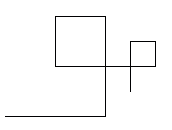
\includegraphics[scale=0.75]{Imatges/figuraS12-5.png}
\noindent
\textsf{\upshape
\begin{tabbing}
$|$ pica $|$\\
pica := Bot nou.\\
pica \= ves: 100 ; \\
\> giraEsquerra: 90 ;\\
\> ves: 100 ;\\
\> giraEsquerra: 90 ;\\
\> ves: 50 ;\\
\> giraEsquerra: 90 ;\\
\> ves: 50 ;\\
\> giraEsquerra: 90 ;\\
\> ves: 100 ;\\
\> giraEsquerra: 90 ;\\
\> ves: 25 ;\\
\> giraEsquerra: 90 ;\\
\> ves: 25 ;\\
\> giraEsquerra: 90 ;\\
\> ves: 50 \\
\end{tabbing}
}
\label{scr12-5}
\end{script}

\begin{center}
\colorbox{black}{\makebox[\textwidth]{  \color{white} {\large {\bfseries Experiment 12-1 (un disseny abstracte senzill)}}}}
\end{center}
\index{disseny abstracte@un disseny abstracte senzill, Experiment}
\index{Experiments!disseny abstracte@un disseny abstracte senzill}
{\small
\noindent
Creeu un mètode anomenat \textsf{patro} que generi la figura de l'\emph{Script}~\ref{scr12-5}}\\
\noindent
\rule{\textwidth}{3pt}
\vspace*{2mm}

Ara podeu utilitzar aquest mètode dins un \emph{script} per dibuixar un disseny més elaborat que podríeu fer servir com a marc ``art nouveau''.
\begin{script}  Un marc art nouveau.
\newline
\newline
\noindent
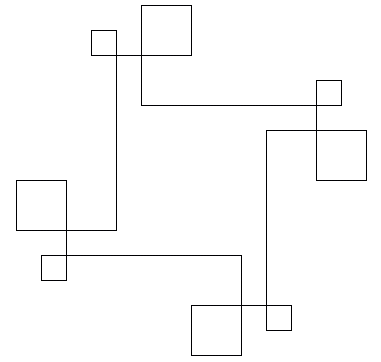
\includegraphics[scale=1.5]{Imatges/figuraS12-6.png}
\noindent
\textsf{\upshape
\begin{tabbing}
$|$ pica $|$\\
pica := Bot nou.\\
4 vegadesRepetir: [ pica patro ; ves: 50 ]\\
\end{tabbing}
}
\label{scr12-6}
\end{script}

Ara el lector astut podria preguntar, ``Per què no creem un mètode, anomenat \textsf{marc50}, per exemple, corresponent a l'\emph{Script}~\ref{scr12-6}?'' Això és possible, ja que \emph{qualsevol mètode creat per a un robot pot ser reutilitzat per qualsevol altre mètode de robots}. Crear aquests mètodes és el tema del proper capítol. \index{dibuixar!figures|)}\index{figures!dibuixar|)}

\begin{center}
\colorbox{black}{\makebox[\textwidth]{  \color{white} {\large {\bfseries Experiment 12-2 (un mètode pel marc art nouveau)}}}}
\end{center}
\index{metode pel marc@un mètode pel marc art nouveau, Experiment}
\index{Experiments!metode pel marc@un mètode pel marc art nouveau}
{\small
\noindent
Creeu un mètode anomenat \textsf{marc50} que generi el disseny de l'\emph{Script}~\ref{scr12-6}}\\
\noindent
\rule{\textwidth}{3pt}

\section{Resum}
\index{compondre mètodes, definició de|seealso{mètodes}}
\begin{itemize}
\item Un \emph{mètode} és una seqüència d'expressions amb nom. Està compost d'un nom, un comentari i una seqüència d'expressions. Un cop s'ha definit un mètode per a robots, qualsevol robot pot executar-lo en resposta a un missatge amb el mateix nom. 
\item El nom d'un mètode sempre hauria de representar què fa el mètode, no com ho fa.
\item Un mètode nou per a robots es crea utilitzant l'\textsf{Explorador de la classe Bot}, que és un editor especial per definir mètodes.
\item Dins d'un mètode la variable \textsf{self} representa l'objecte que rep el missatge. Quan el codi del mètode necessita enviar un missatge al receptor, el missatge s'hauria d'enviar a \textsf{self}.
\end{itemize}

\section{Glossari} \index{Glossari per a mètodes}

\begin{itemize}
\item[] \textbf{Categories de Mètodes} Una categoria de mètodes és una carpeta on els mètodes es classifiquen. Les categories us ajuden a trobar els mètodes més ràpidament.
\item[] \textbf{Mètode} Un mètode representa una seqüència d'expressions que un objecte pot executar. Un mètode té un nom. S'executa quan l'objecte rep un missatge amb el mateix nom.
\item[] \textbf{Explorador de la Classe Bot} Un \textsf{Explorador de la Classe Bot} és una eina especial per veure i editar mètodes.
\item[] \textbf{Comentari} Un comentari és un text entre cometes dobles que explica el propòsit d'un mètode.
\item[] \textbf{self} La variable \textsf{self} està predefinida a Smalltalk. Sempre representa el receptor del missatge dins de la definició d'un mètode.
\end{itemize}

\chapter{Combinar mètodes}
\label{cap13}

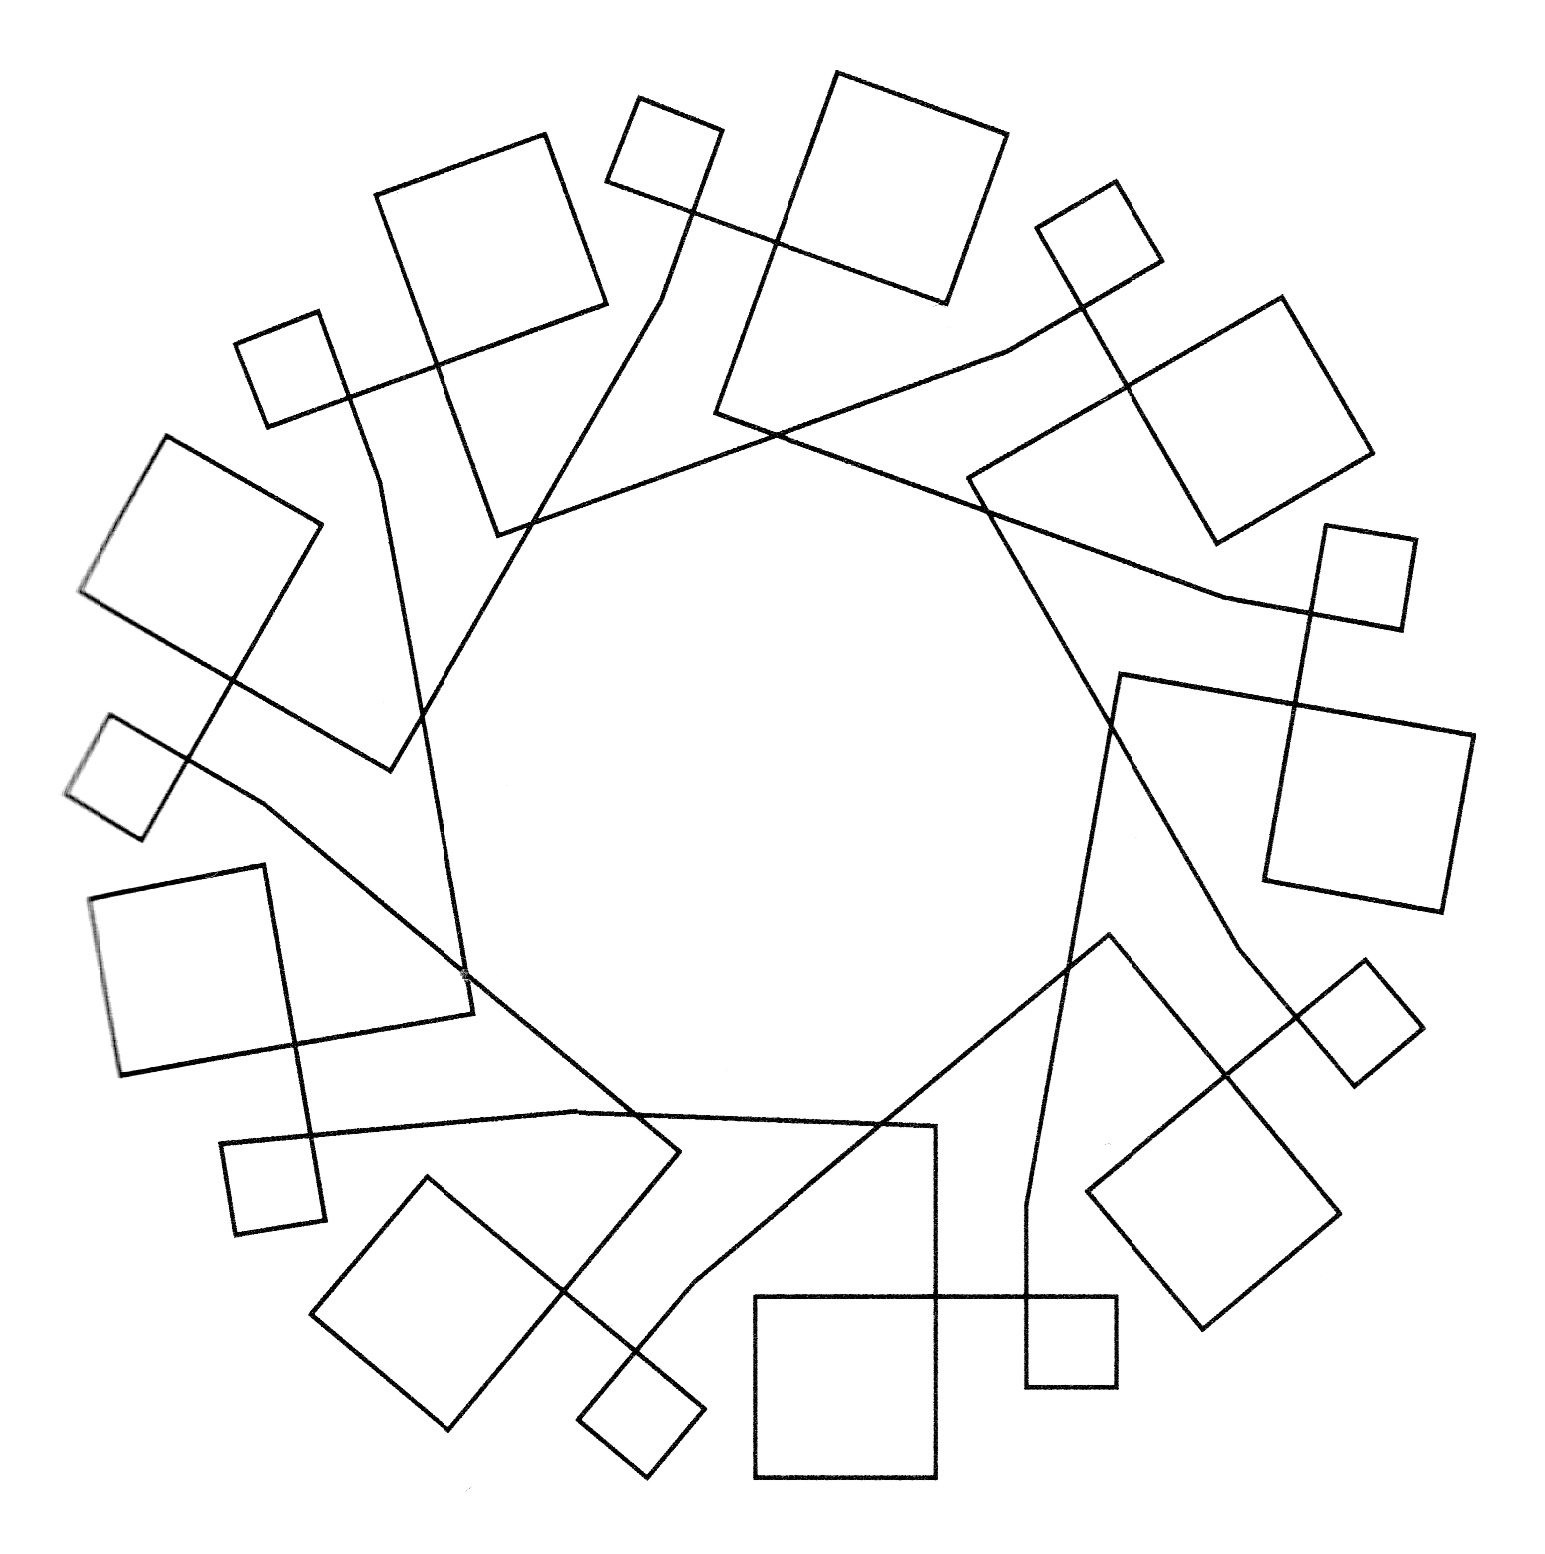
\includegraphics[scale=0.10]{Imatges/figura13-0.jpg}

Heu après al capítol~\ref{cap12} com definir mètodes. Vam ensenyar-vos que definir mètodes és útil i interessant ja que (1) els mètodes us estalvien haver de reescriure \emph{scripts}, la qual cosa requereix temps i és susceptible d'introduir errors, i (2) els mètodes poden ser utilitzats i reutilitzats per robots diferents. L'altre gran avantatge d'utilitzar mètodes és la possibilitat d'emprar mètodes dins d'altres mètodes, és a dir, cridar un o més mètodes ja existents com a part de la definició d'un mètode nou. La reutilització de mètodes és el que explorarem en aquest capítol.

És extremadament important que siguem capaços de reutilitzar mètodes, ja que podem definir un mètode en termes d'un altre sense haver de conèixer tots els detalls de la definició d'aquest altre mètode. Ens podem limitar a cridar-lo i demanar que faci allò pel que ha estat dissenyat.

\section{Res de nou: Revisitar el mètode \textsf{quadrat}}
\index{compondre mètodes, definició de}
Tenir mètodes que cridin altres mètodes (cosa que anomenem \emph{compondre mètodes}) és natural i no és realment nou. De fet, és el que vau fer al capítol~\ref{cap12} quan vau definir un mètode! El mètode \textsf{quadrat} inclou a la seva definició crides als mètodes \textsf{giraEsquerra:}, \textsf{ves:} i \textsf{vegadesRepetir:} (com es pot veure al Mètode~\ref{met13-1}). Així, fins i tot el simple mètode \textsf{quadrat} està definit en termes d'altres mètodes, i no ens ha calgut saber com estan definits \textsf{giraEsquerra:}, \textsf{ves:} i \textsf{vegadesRepetir:}. Només ens calia conèixer què feien. Per tant, ja hem acabat aquest capítol, sense res més a fer que divertir-nos una mica.
\begin{metode}
\noindent
\textsf{\upshape
\begin{tabbing}
\hspace{5mm} \= \hspace{10mm} \= \kill
{\bfseries quadrat}\\
\> {\itshape ``Dibuixa un quadrat amb costats de mida 100 píxels''}\\
\\
\> 4 vegadesRepetir:\\
\>\> [  self \= ves: 100 ; \\
\>\> \> giraEsquerra: 90  ]\\
\end{tabbing}
}
\label{met13-1}
\end{metode}

\section{Altres patrons gràfics}
\index{figures!exemples de|(}
Al capítol~\ref{cap12} us vam demanar de definir el mètode \textsf{patro}, que dibuixa un senzill patró abstracte (veure \emph{Script}~\ref{scr12-5}). Ara us demanarem de fer alguns experiments per generar més dibuixos definint més mètodes. \index{patro4, mètode!definir|(}

\begin{center}
\colorbox{black}{\makebox[\textwidth]{  \color{white} {\large {\bfseries Experiment 13-1}}}}
\end{center}
{\small
\noindent
Definiu un mètode \textsf{patro4} que cridi a \textsf{patro} quatre vegades per generar la figura de més avall. Utilitzareu aquest mètode més tard, en un altre \emph{script}. Després que hagueu creat el mètode \textsf{patro4}, utilitzeu l'\emph{script} de tres línies següent per fer que pica dibuixi la figura}\\
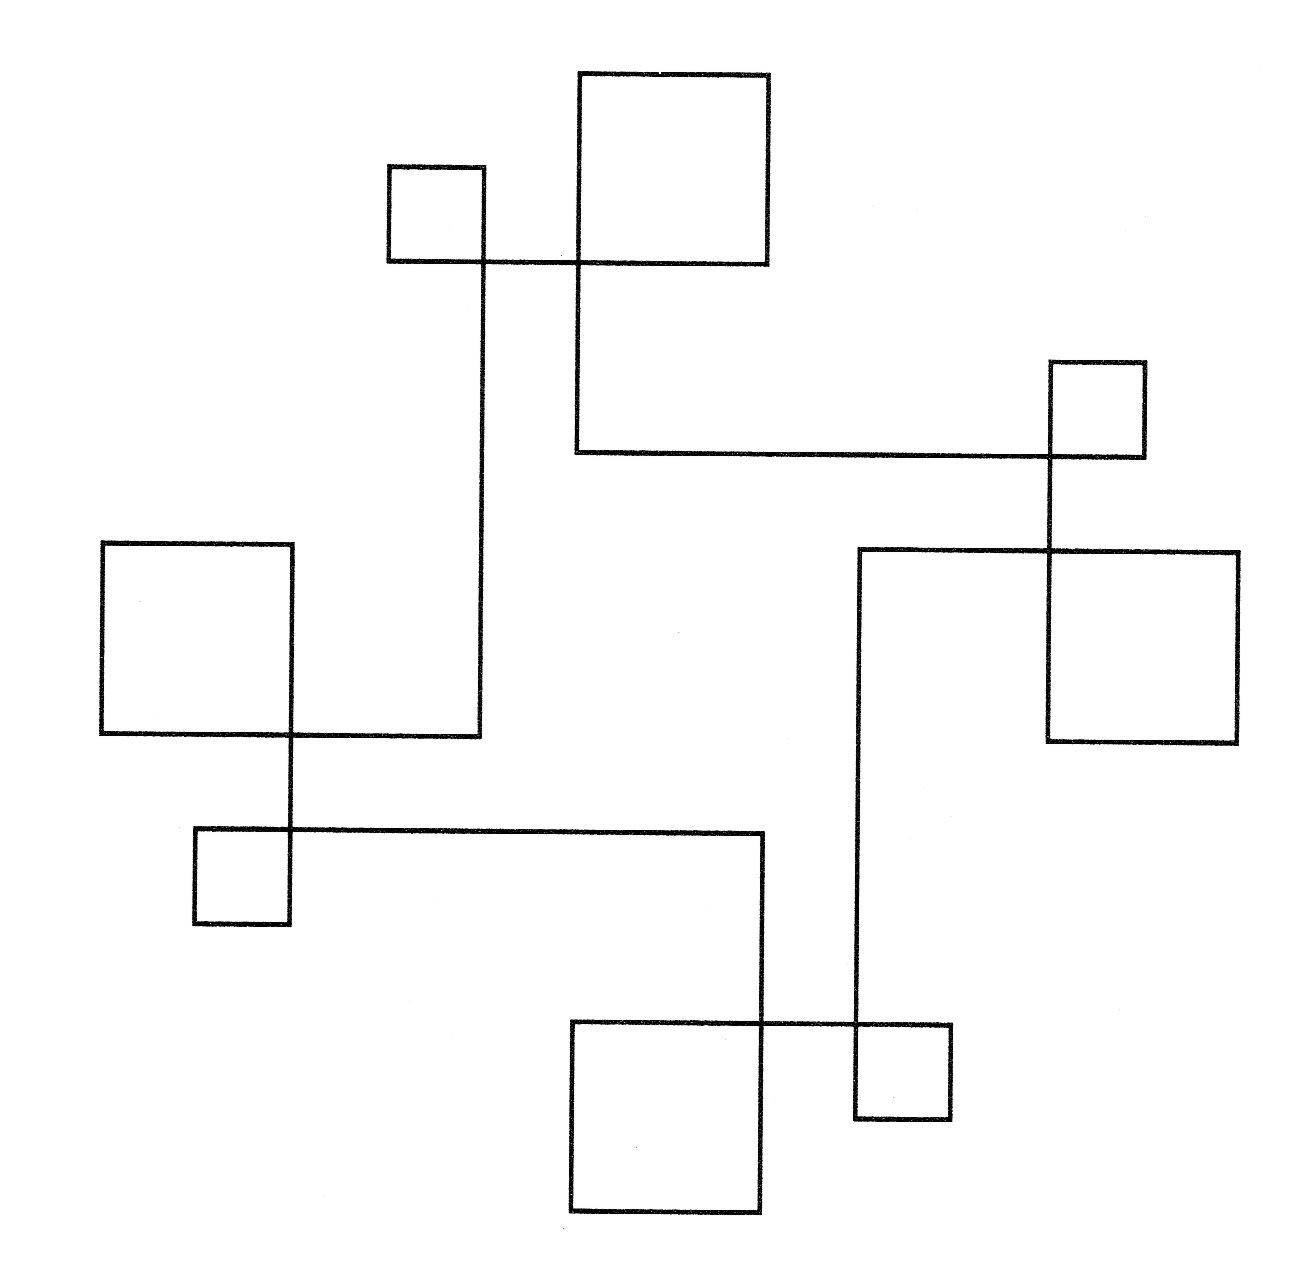
\includegraphics[scale=0.1]{Imatges/figuraE13-1.jpg} 
\noindent
{\small
\textsf{
\\$|$ pica $|$\\
pica := Bot nou.\\
pica patro4\\
}}
\noindent
\rule{\textwidth}{3pt}

\begin{center}
\colorbox{black}{\makebox[\textwidth]{  \color{white} {\large {\bfseries Experiment 13-2 (una roda)}}}}
\end{center}
\index{roda @una roda, Experiment}
\index{Experiments!roda @una roda}
{\small
\noindent
Definiu un mètode anomenat \textsf{patroInclinat} que generi la figura que podeu veure al començament d'aquest capítol, que sembla lleugerament una sínia. Pista: haureu de cridar a \textsf{patro} nou vegades, i l'angle que haureu de girar entre crides és de 10 graus.}\\
\noindent
\rule{\textwidth}{3pt}

\begin{center}
\colorbox{black}{\makebox[\textwidth]{  \color{white} {\large {\bfseries Experiment 13-3 (duplicar el marc)}}}}
\end{center}
\index{duplicar el marc, Experiment}
\index{Experiments!duplicar el marc}
\index{dobleMarc mètode, definir|(}
{\small
\noindent
Definiu el mètode \textsf{dobleMarc}, que podeu trobar més avall, per dibuixar la figura que veieu abans de la definició del mètode}\\
\newline
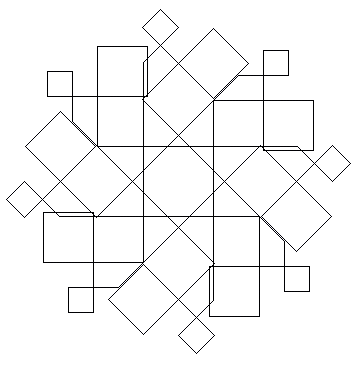
\includegraphics[scale=1.5]{Imatges/figuraE13-3.png} 
\noindent
{\small
\textsf{
\begin{tabbing}
\hspace{5mm} \= \hspace{10mm} \= \kill
{\bfseries dobleMarc}\\
\\
\> 8 vegadesRepetir:\\
\>\> [  self patro. \\
\>\> self giraEsquerra: 45.\\
\>\>self ves: 100  ]\\
\end{tabbing}
}}

\noindent
\rule{\textwidth}{3pt}

\section{Què us diuen aquests experiments?}
\index{metodes@mètodes!utilitzar i reutilitzar}
\index{patrons|see{figures}}
\index{figures!exemples de|)}
\index{patro4, mètode!definir|)}
Què podeu aprendre dels experiments que acabeu de fer?. Com podeu veure en els mètodes \textsf{patro4}, \textsf{patroInclinat} i \textsf{dobleMarc}, el mètode \textsf{patro} ha estat definit una sola vegada, i \emph{reutiltzat diverses vegades} a mètodes diferents. Definir \textsf{patro} com a mètode us permet (1) definir-lo només una vegada, (2) reutilitzar-lo en contextos diversos, i (3) no introduir errors a causa de copiar una vegada i una altra aquest mètode.\index{patroInclinat mètode, significat de}

Si pareu atenció a la definició del mètode \textsf{dobleMarc}, veureu que està definit en termes del mètode \textsf{patro}, definit ell mateix en termes d'altres mètodes, com \textsf{ves:} i \textsf{giraEsquerra:}. De fet, un mètode complex sovint es defineix en termes de mètodes més simples, que alhora estan definits en termes de mètodes encara més senzills, que alhora estan definits en termes de mètodes encara més senzills, que alhora\dots L'avantatge d'això és que els mètodes senzills són més fàcils d'entendre i definir que els mètodes complexos, i la tècnica de definir mètodes en termes de mètodes més simples limita el grau de complexitat de qualsevol mètode. Al capítol~\ref{cap16} us ensenyarem que per resoldre un problema, és avantatjós descompondre el problema en subproblemes més senzills, resoldre aquests subproblemes, i després utilitzar les solucions als subproblemes per resoldre el problema principal.

És essencial entendre que per definir el mètode \textsf{dobleMarc}, no us cal conèixer com està definit \textsf{patro}. Només heu de saber què fa i com utilitzar-lo! Quan definim un mètode estem donant un sol nom a una seqüència de missatges, la qual cosa redueix el nombre de detalls que hem de tenir en compte. Només ens cal recordar què fa el mètode, no com ho fa. Direm que estem construint una \emph{abstracció} sobre els detalls de la definició.
\index{abstracció, construint sobre els detalls de la definició}
Per deixar-ho clar, hem escrit el mètode \textsf{dobleMarc} sense cridar el mètode \textsf{patro}, copiant-ne directament la definició (mostrada en itàlica). Compareu \textsf{dobleMarcSenseCridarPatro} (Mètode~\ref{met13-2}) amb el mètode \textsf{dobleMarc}. La nova versió sense \textsf{patro} no només és més llarga, sinó que per a la majoria de la gent és més confusa i difícil d'entendre.\index{metodes@mètodes!cridar altres mètodes amb}

Ara imagineu què passaria si féssim el mateix amb el codi de \textsf{giraDreta:}, \textsf{giraEsquerra:} i \textsf{ves:} --ja que aquests són també mètodes. Seria un malson! Hi hauria tants detalls que estaríem perduts tota l'estona.
%%COMPTE
\newpage
%%COMPTE
\begin{metode} Crear el doble marc sense l'abstracció del mètode patro.
\noindent
\textsf{\upshape
\begin{tabbing}
\hspace{5mm} \= \hspace{10mm} \= \kill
{\bfseries dobleMarcSenseCridarPatro}\\
\\
\> 8 vegadesRepetir:\\
\>\> {\itshape [  self  ves: 100.} \\
\>\> {\itshape self giraDreta: 90.}\\
\>\> {\itshape  self  ves: 100.} \\
\>\> {\itshape self giraDreta: 90.}\\
\>\> {\itshape  self  ves: 50.} \\
\>\> {\itshape self giraDreta: 90.}\\
\>\> {\itshape  self  ves: 50.} \\
\>\> {\itshape self giraDreta: 90.}\\
\>\> {\itshape  self  ves: 100.} \\
\>\> {\itshape self giraDreta: 90.}\\
\>\> {\itshape  self  ves: 25.} \\
\>\> {\itshape self giraDreta: 90.}\\
\>\> {\itshape  self  ves: 25.} \\
\>\> {\itshape self giraDreta: 90.}\\
\>\> {\itshape  self  ves: 50.} \\
\>\> self giraEsquerra: 45.\\
\>\> self ves: 100  ]\\
\end{tabbing}
}
\label{met13-2}
\end{metode}
\index{dobleMarc mètode, definir|)}
\index{dobleMarcSenseCridarPatro mètode, definir}
\noindent
\rule{\textwidth}{2pt}
\noindent
\textbf{Important!} Quan escriviu un nou mètode, aquest pot cridar altres mètodes. Podeu utilitzar un mètode sense conèixer com està definit. Després d'acabar d'escriure un mètode, podeu cridar-lo quan definiu un altre mètode.\\
\noindent
\rule{\textwidth}{2pt}

\section{Quadrats a tot arreu}
\index{quadrat: mètode!definir mètodes amb}
\index{metodes@mètodes!definir amb el mètode quadrat}
Ara és el moment de practicar. Definiu els següents mètodes utilitzant el mètode \textsf{quadrat}.

\begin{center}
\colorbox{black}{\makebox[\textwidth]{  \color{white} {\large {\bfseries Experiment 13-4 (algunes capses)}}}}
\end{center}
\index{algunes capses, Experiment}
\index{Experiments!algunes capses}
{\small
\noindent
Definiu els mètodes \textsf{capsa} i \textsf{capsaSeparada} que generi els dibuixos de la figura~\ref{fig1301}}\\
\noindent
\rule{\textwidth}{3pt}

\begin{figure}[h!]
\begin{center}
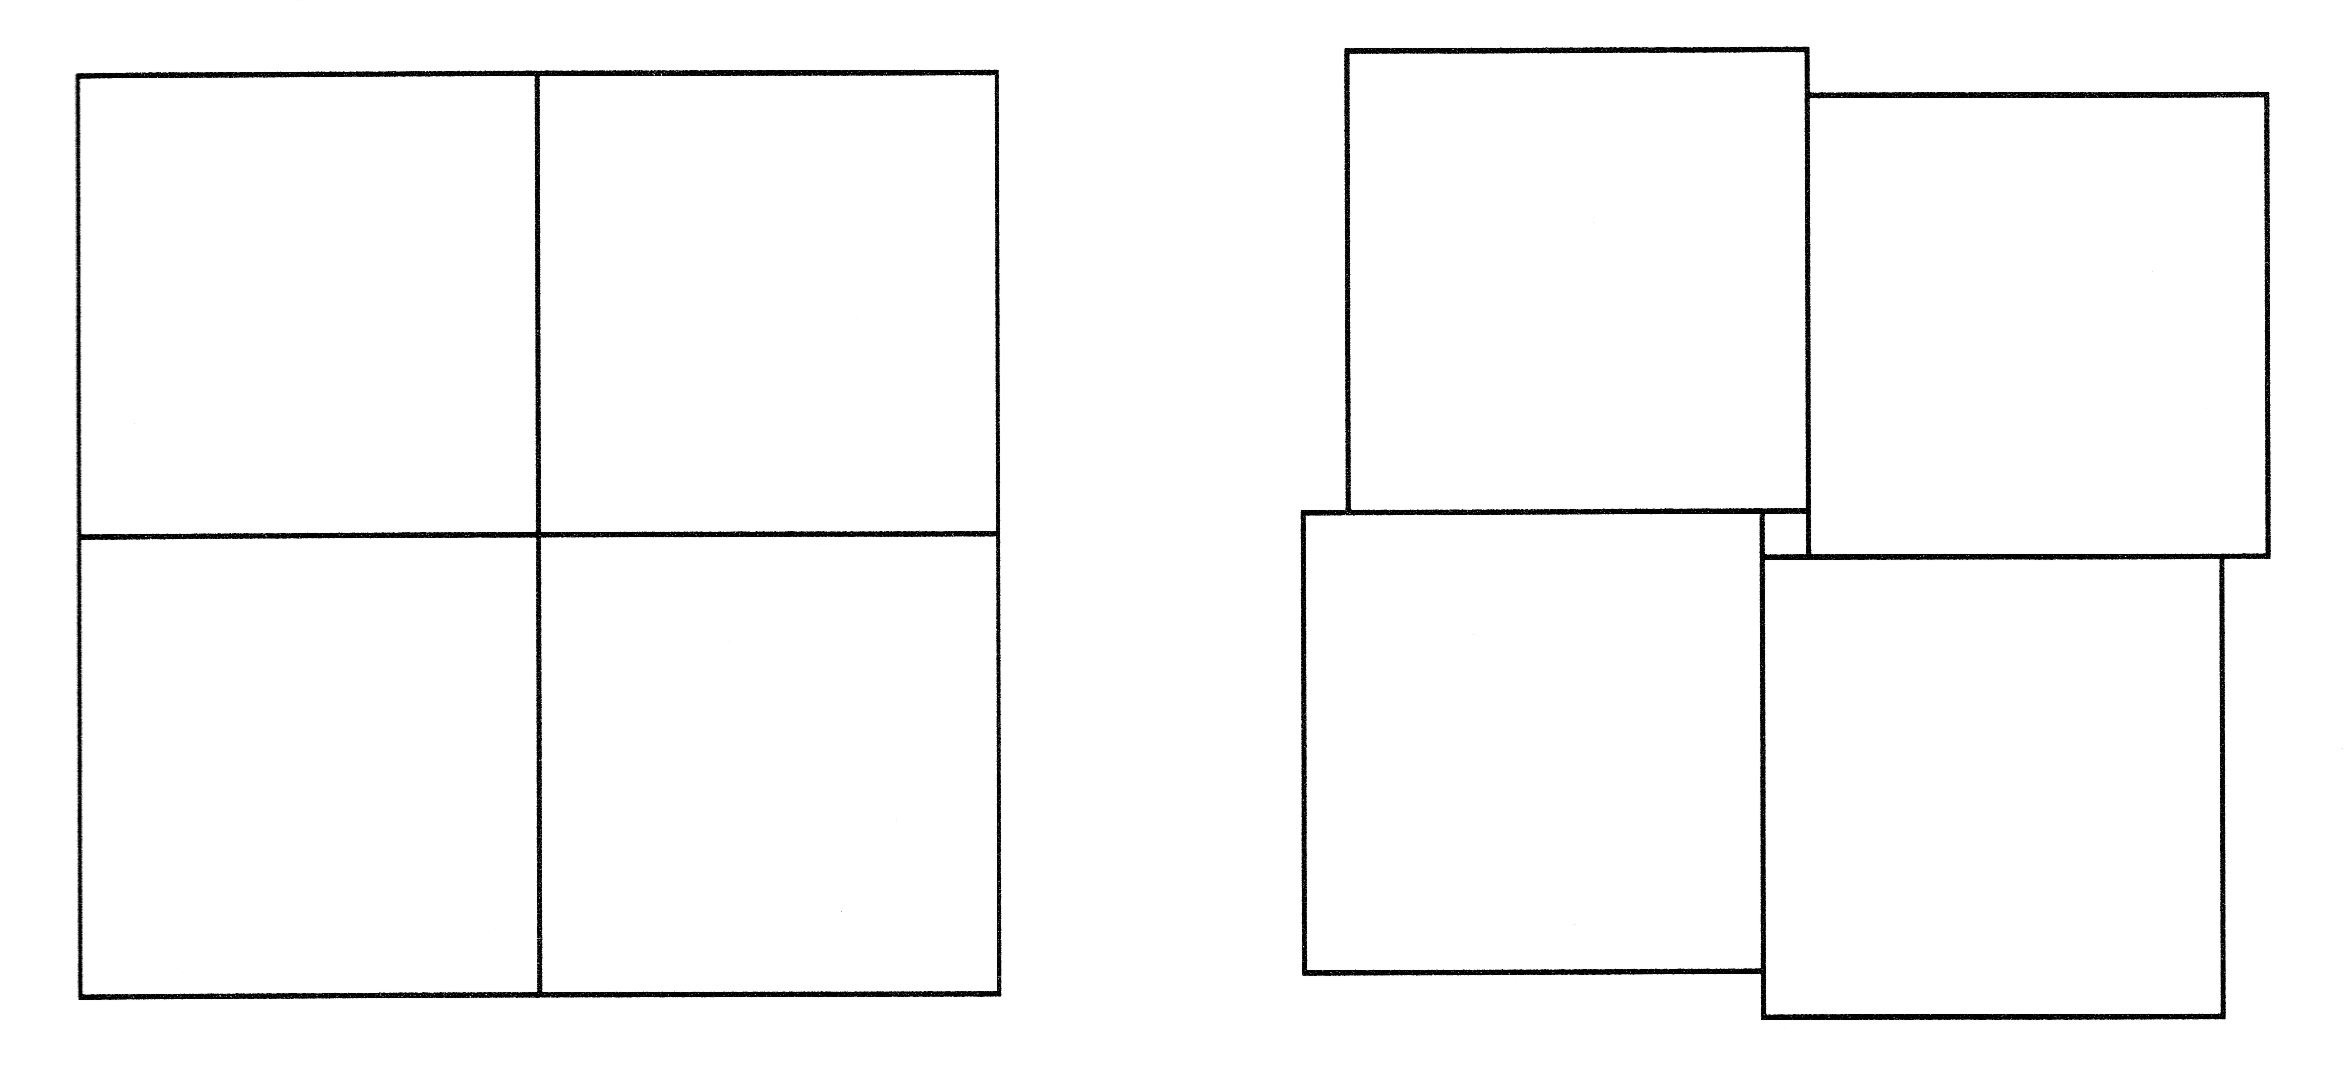
\includegraphics[scale=0.1]{Imatges/figura13-1.jpg}
\end{center}
\caption{Capses}
\label{fig1301}
\end{figure}

\begin{center}
\colorbox{black}{\makebox[\textwidth]{  \color{white} {\large {\bfseries Experiment 13-5 (trieu vosaltres)}}}}
\end{center}
\index{trieu vosaltres, Experiment}
\index{Experiments!trieu vosaltres}
{\small
\noindent
Utilitzeu els mètodes que ja heu definit per generar diverses figures. Vosaltres trieu quines figures. Divertiu-vos!}\\
\noindent
\rule{\textwidth}{3pt}

\begin{figure}[h!]
\begin{center}
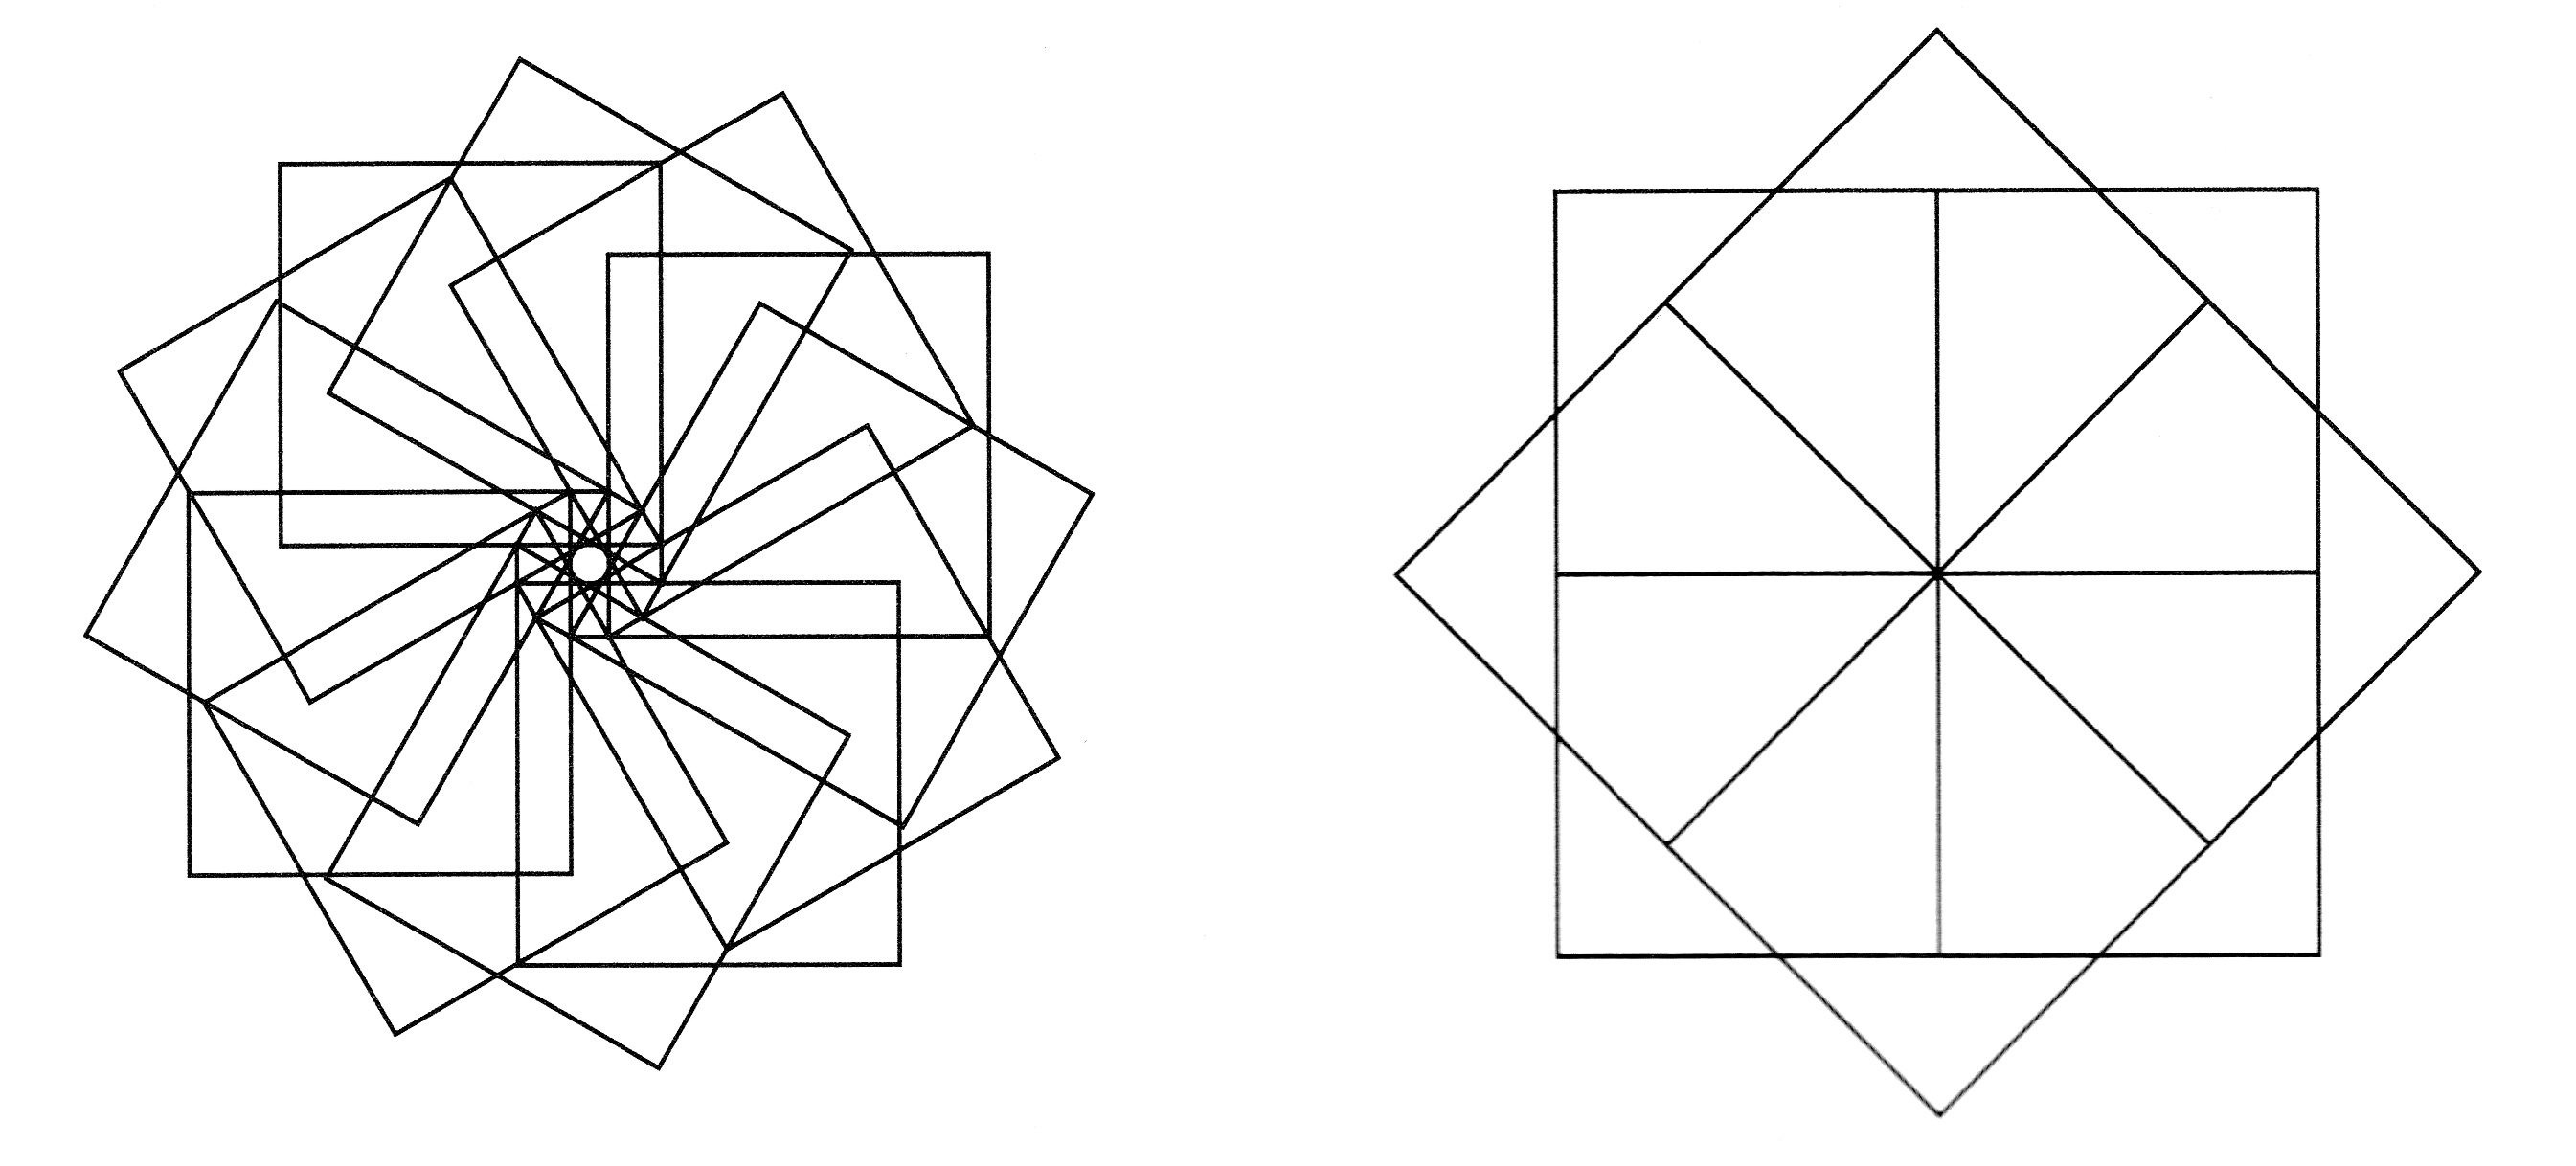
\includegraphics[scale=0.1]{Imatges/figura13-2.jpg}
\end{center}
\caption{Estrelles}
\label{fig1302}
\end{figure}

\begin{center}
\colorbox{black}{\makebox[\textwidth]{  \color{white} {\large {\bfseries Experiment 13-6 (una estrella)}}}}
\end{center}
\index{estrella @una estrella, Experiment}
\index{Experiments!estrella @una estrella}
\index{metode@mètode capsa, definir mètode estrella amb}
{\small
\noindent
Utilitzant el mètode \textsf{capsa}, experimenteu i definiu un mètode \textsf{estrella} per generar el dibuix de la dreta de la figura~\ref{fig1302}}\\
\noindent
\rule{\textwidth}{3pt}

\section{Resum}

\begin{itemize}
\item Quan definiu un mètode nou, pot cridar a altres mètodes.
\item Podeu utilitzar un mètode sense conèixer com està definit; només us cal saber què fa.
\item Després de definir un mètode, el podeu cridar quan definiu altres mètodes.
\item Amagar els detalls d'un mètode tot donant-li un nom és el que anomenem \emph{abstracció}.
\end{itemize}

\chapter{Paràmetres i arguments}
\label{cap14}

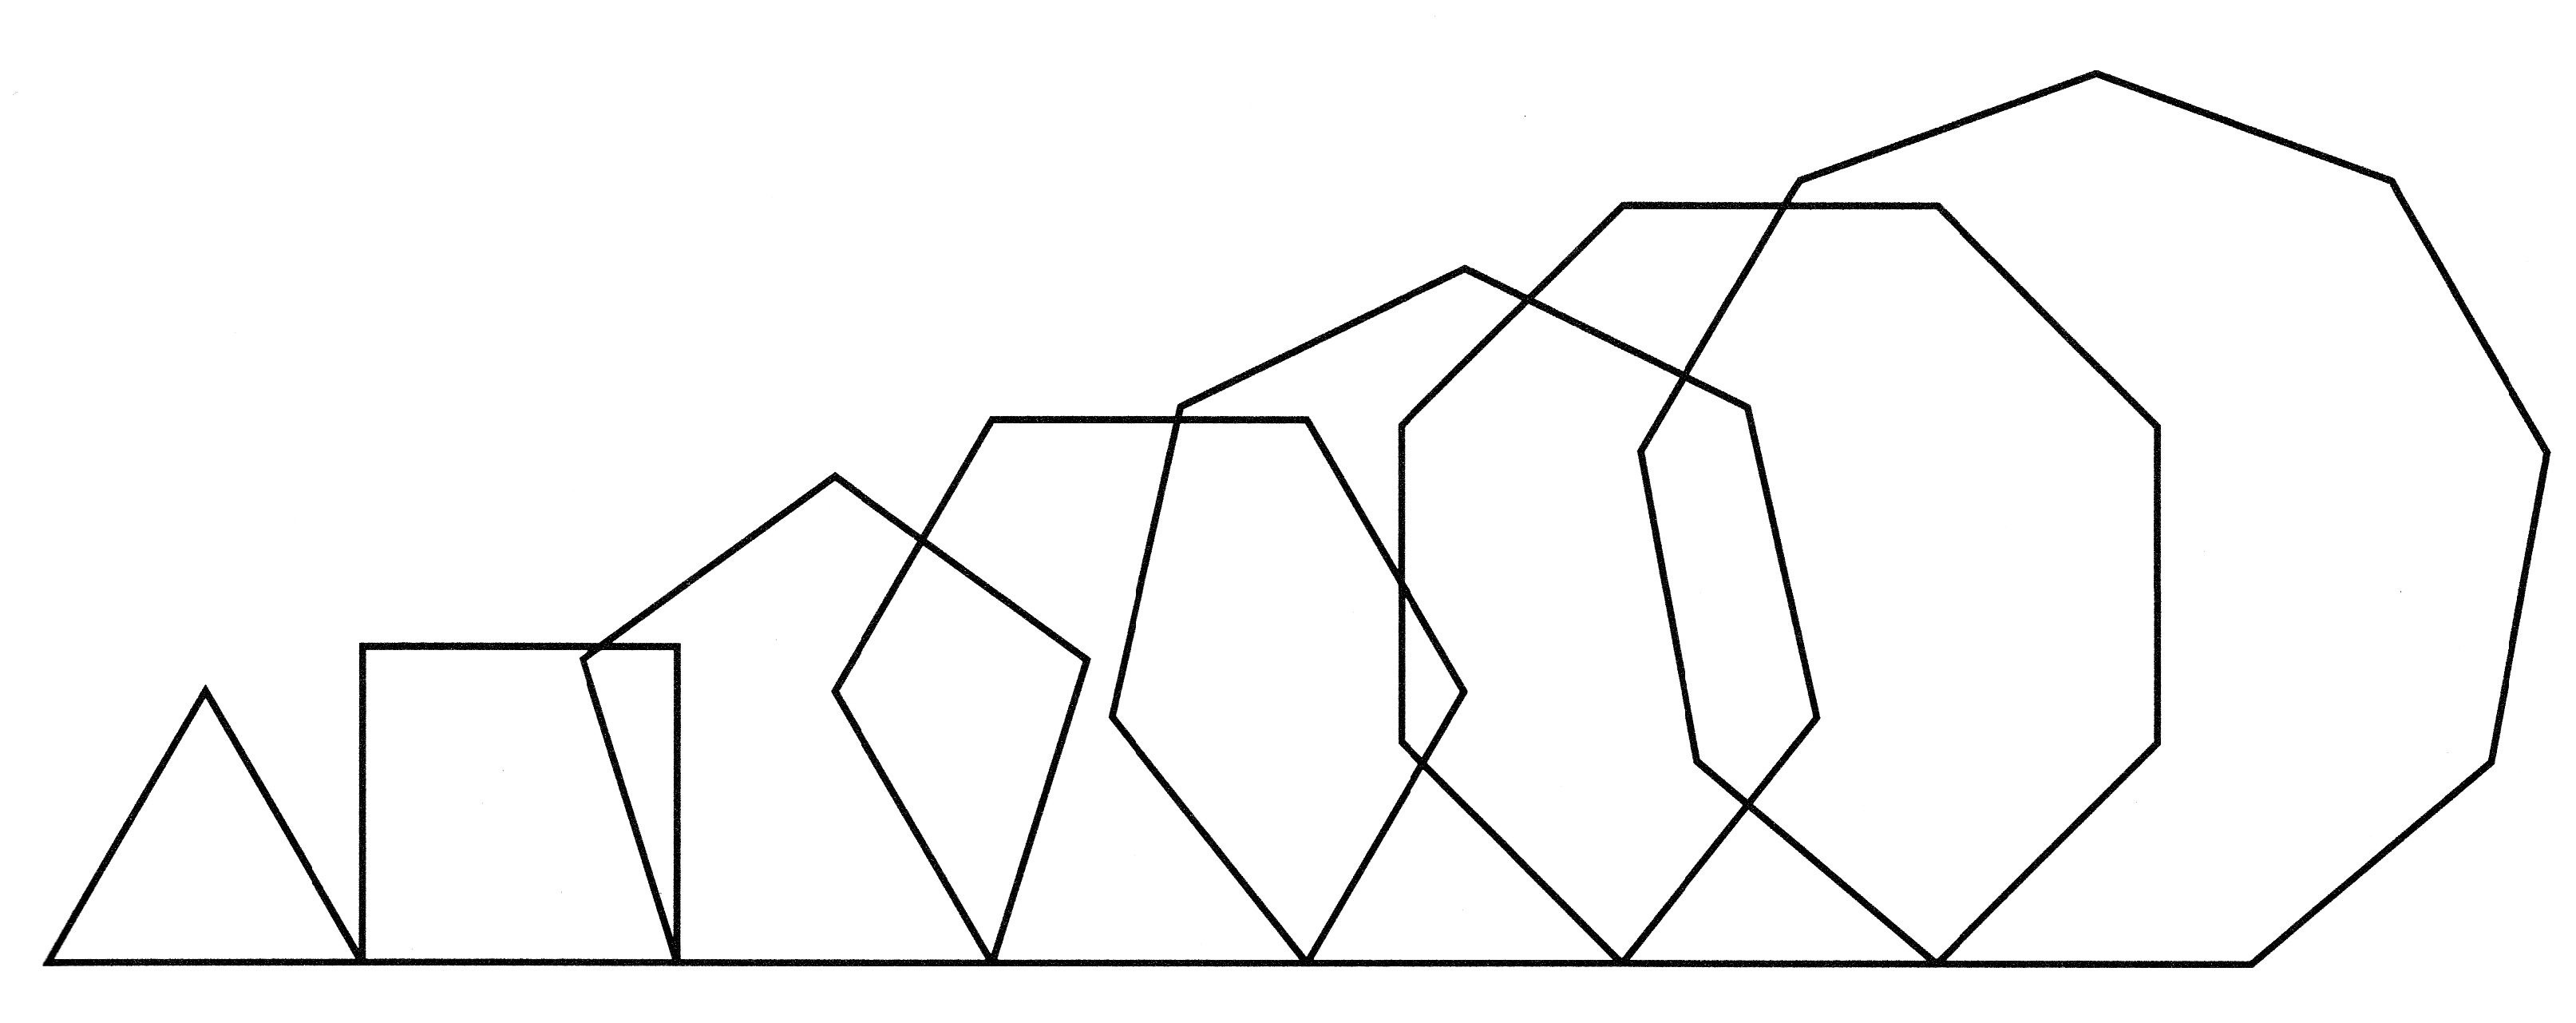
\includegraphics[scale=0.13]{Imatges/figura14-0.jpg}

En molts dels \emph{scripts} que ja heu escrit, heu enviat missatges amb \emph{arguments}. Per exemple, al missatge \textsf{ves: 100} vau especificar que un robot s'hauria de moure una distància de 100 píxels, i l'argument del missatge és per tant \textsf{100}. Malgrat que heu après com definir mètodes, no heu après encara com definir mètodes que requereixin un o més arguments.

En aquest capítol aprendreu com definir mètodes el comportament dels quals depengui dels valors dels arguments del missatge. Direm que aquests mètodes tenen \emph{paràmetres}, i que el seu comportament està parametritzat. Els paràmetres d'un mètode actuen com a receptacles a la definició del mètode, i aquests receptacles s'omplen amb els arguments del missatge quan el missatge és enviat. Primer definirem un mètode amb un paràmetre, i l'invocarem. Després l'analitzarem.

\section{Què és un paràmetre?}
\index{parametres@paràmetres!definició de}
\index{arguments!utilitzar en mètodes}
\index{missatge, selectors de!utilitzar dos punts (:) amb}
\index{metodes@mètodes!utilitzar arguments amb}
El mètode \textsf{quadrat} definit al capítol~\ref{cap12} és una mica limitat, ja que la mida del quadrat es fixa una vegada i ja no es pot modificar. Us podeu haver preguntat, ``Què podríem fer per poder dibuixar un quadrat de costats de mida 300 píxels, o 175, o 225, o fins i tot 23 píxels?'' No hi ha res que us impedeixi definir els mètodes \textsf{quadrat300}, \textsf{quadrat175}, \textsf{quadrat225}, \textsf{quadrat23} i així successivament.

Crear múltiples mètodes \textsf{quadrat}, però, no resol el problema de manera satisfactòria. Seria molt incòmode si haguéssim de definir un mètode nou cada cop que volguéssim dibuixar un quadrat de mida diferent. El que realment volem és tenir un mètode general per dibuixar quadrats, que permeti a l'usuari especificar la mida del costat del quadrat en el moment de cridar al mètode. D'aquesta manera, no hauríem de definir un mètode nou per a cada quadrat de mida diferent.

El que necessitem és substituir la mida fixa del costat del quadrat per una mena de variable el valor de la qual serà assignat en el moment d'enviar el missatge, no abans. Aquesta mena de variable existeix en molts llenguatges de programació. S'anomena un \emph{paràmetre}. Un paràmetre d'un mètode és una variable especial que pot prendre qualsevol valor \emph{en el moment de l'enviament del missatge}. Així doncs, serveix com a receptacle quan es defineix el mètode i per tant no rep cap valor en la definició del missatge.

Això us hauria de sonar. Després de tot, ja sabeu que mètodes com \textsf{ves:} i \textsf{giraEsquerra:} necessiten un argument (una distància o un angle) en el moment de l'enviament del missatge. Cada vegada que escriviu una expressió com \textsf{pica giraEsquerra: 90}, \textsf{pica giraEsquerra: 32} o \textsf{daly giraEsquerra: 65} afegiu en el missatge el valor d'un angle com a argument, i aleshores el \emph{mètode} \textsf{giraEsquerra:} utilitza aquest valor per decidir quin angle ha de girar el robot. De fet, en totes i cada una d'aquestes expressions, és el \emph{mateix} mètode \textsf{giraEsquerra:} el que s'executa, cada cop amb un \emph{valor diferent} per a l'angle que \textsf{pica} o \textsf{daly} ha de girar. Ser capaç d'especificar diferents angles en enviaments de missatge diferents utilitzant el mateix selector de missatge \textsf{giraEsquerra:} és una valuosa propietat  del mètode \textsf{giraEsquerra:}. Vosaltres voldríeu que el mètode per dibuixar quadrats tingués aquestes propietats, igualment amb altres mètodes que pugueu definir. I els vostres mètodes les tindran aquestes propietats, tan aviat com expliquem com definir mètodes que, com el mètode \textsf{giraEsquerra:}, puguin tenir un o més arguments en temps d'execució.\index{metodes@mètodes!definir amb múltiples arguments}

\subsection{Un mètode per dibuixar quadrats}
\index{: (dos punts)!utilitzar en selectors de missatge}
\index{dos punts (:)!utilitzar en selectors de missatge}
\index{metodes@mètodes!per dibuixar quadrats|(}
\index{quadrats!dibuixar amb mètodes|(}
Ja heu vist que en Smalltalk, el nom d'un selector de missatge acaba en ``dos punts'' (:) per indicar que el missatge necessita un argument. Igualment, el nom del mètode corresponent a aquest selector de missatge també acaba en ``dos punts'' (:), i a la definició del mètode, un paràmetre és utilitzat com a receptacle per a l'argument del missatge. Així, si voleu crear un mètode per dibuixar un quadrat de mida arbitrària, podríeu utilitzar \textsf{quadrat:} com a nom i \textsf{midaCostat} com a paràmetre. Podeu definir aleshores el mètode \textsf{quadrat:} com veieu al Mètode~\ref{met14-1}. Aquest mètode s'utilitza en l'\emph{Script}~\ref{scr14-1}, en el qual \textsf{pica} dibuixa dos quadrats, un de costat de mida 10 i l'altre de costat de mida 20.
\begin{metode} El mètode \textsf{\upshape quadrat:} utilitza el paràmetre \textsf{\upshape midaCostat} per dibuixar un quadrat de mida arbitrària.
\noindent
\textsf{\upshape
\begin{tabbing}
\hspace{5mm} \= \hspace{10mm} \= \kill
quadrat: {\bfseries {\itshape midaCostat}}\\
\> {\itshape ``Dibuixa un quadrat amb costats de la mida donada''}\\
\\
\> 4 vegadesRepetir:\\
\>\> [  self  ves: {\bfseries {\itshape midaCostat}} .\\
\>\> self giraEsquerra: 90  ]\\
\end{tabbing}
}
\label{met14-1}
\index{midaCostat paràmetre!utilitzar al mètode quadrat:}
\index{quadrat: mètode!utilitzar el paràmetre midaCostat amb}
\end{metode}

\begin{script}  El mètode \textsf{\upshape quadrat:} és utilitzat per dibuixar quadrats de diferentes mides.
\textsf{\upshape
\begin{tabbing}
\hspace{5mm} \= \kill
$|$ pica $|$\\
pica := Bot nou.\\
pica quadrat: 10.\\
pica ves: 300.\\
pica quadrat: 20.\\
\end{tabbing}
}
\label{scr14-1}
\end{script}

Ara analitzem la definició del mètode \textsf{quadrat:} al Mètode~\ref{met14-1}. Per definir un mètode que requereix un argument, cal que el nom del mètode acabi amb ``dos punts'' i sigui seguit del nom del paràmetre, que aquí és \textsf{midaCostat}.

El paràmetre representa una variable el valor de la qual es defineix quan el missatge és enviat (no quan el mètode és definit). A l'\emph{Script}~\ref{scr14-1}, quan s'envia el missatge \textsf{quadrat: 10}, el paràmetre \textsf{midaCostat} pren el valor \textsf{10}. Després, quan s'enviï el missatge \textsf{quadrat: 20}, \textsf{midaCostat} prendrà el valor \textsf{20}. Els paràmetres no es declaren explícitament utilitzant les barres verticals \textbar  \hspace{2mm} \textbar, com les variables normals dels \emph{scripts}.

Al Mètode~\ref{met14-1}, el nom del paràmetre és \textsf{midaCostat}. El nom del paràmetre hauria de triar-se per indicar per a què s'utilitza. Podríeu haver-lo anomenat \textsf{longitud}, com en el Mètode~\ref{met14-2} (o \textsf{mida}, o qualsevol altra cosa), sempre i quan substituíssiu totes les aparicions de \textsf{midaCostat} dins del cos del mètode per \textsf{longitud}. Fixeu-vos que el Mètode~\ref{met14-1} i el Mètode~\ref{met14-2} produeixen \emph{exactament} els mateixos resultats. Això és degut al fet que \textsf{midaCostat} i \textsf{longitud} són noms per a exactament la mateixa cosa: el paràmetre del mètode \textsf{quadrat:}.\index{metodes@mètodes!per dibuixar quadrats|)}
\newpage
\begin{metode} 
\noindent
\textsf{\upshape
\begin{tabbing}
\hspace{5mm} \= \hspace{10mm} \= \kill
quadrat: {\bfseries {\itshape longitud}}\\
\> {\itshape ``Dibuixa un quadrat amb costats de la mida donada''}\\
\\
\> 4 vegadesRepetir:\\
\>\> [  self  ves: {\bfseries {\itshape longitud}} .\\
\>\> self giraEsquerra: 90  ]\\
\end{tabbing}
}
\label{met14-2}
\end{metode}

\section{Practiqueu amb els paràmetres}
\index{parametres@paràmetres!utilitzar}
Ara és moment de practicar una mica. Comencem amb un exercici senzill.

\begin{center}
\colorbox{black}{\makebox[\textwidth]{  \color{white} {\large {\bfseries Experiment 14-1 (un mètode per dibuixar un hexàgon)}}}}
\end{center}
\index{metode per dibuixar un hexàgon@un mètode per dibuixar un hexàgon, Experiment}
\index{Experiments!metode per dibuixar un hexàgon@un mètode per dibuixar un hexàgon}
\index{hexàgons!dibuixar amb paràmetres}
{\small
\noindent
Definiu un mètode \textsf{hexagon:}, que dibuixa un hexàgon amb la mida dels costats com a argument}
\begin{center}
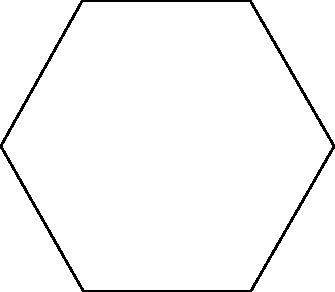
\includegraphics[scale=1]{Imatges/figuraE14-1.pdf} 
\end{center}
\noindent
\rule{\textwidth}{3pt}
\newpage
\begin{center}
\colorbox{black}{\makebox[\textwidth]{  \color{white} {\large {\bfseries Experiment 14-2 (un mètode per dibuixar una creu)}}}}
\end{center}
\index{metode per dibuixar una creu@un mètode per dibuixar una creu, Experiment}
\index{Experiments!metode per dibuixar una creu@un mètode per dibuixar una creu}
\index{creu, dibuixar amb paràmetres}
{\small
\noindent
Transformeu l'\emph{script} que us donem més avall en un mètode anomenat \textsf{creu:} que dibuixa una creu amb la mida d'un dels seus braços com a argument. Després, hauríeu d'executar l'expressió \textsf{pica creu: 100}. Pista: fixeu-vos que $50 = 100 / 2$. Un bon nom per al paràmetre seria \textsf{longitudBraç}.}\\

\includegraphics[scale=0.35]{Imatges/figuraE14-2.png} 
\noindent
{\small
\textsf{
\begin{tabbing}
\hspace{5mm} \= \kill
$|$ pica $|$\\
pica := Bot nou.\\
4 vegadesRepetir:\\
\> [ pica ves: 50.\\
\> pica giraEsquerra: 90.\\
\> pica ves: 100.\\
\> pica giraDreta: 90.\\
\> pica ves: 100.\\
\> pica giraDreta: 90.\\
\> pica ves: 50 ]
\end{tabbing}
}}
\noindent
\rule{\textwidth}{3pt}

\section{Variables en mètodes}
\index{variables!metodes@en mètodes|(}
\index{metodes@mètodes!variables en|(}
\index{parametres@paràmetres!utilitzar en polígons}
\index{poligon@polígon!utilitzar variables i paràmetres amb}
Tal com hem fet servir variables en els nostres \emph{scripts} per anomenar algunes quantitats, també podem utilitzar variables en mètodes pel mateix propòsit. Si volguéssim dir a pica que dibuixés un polígon amb costats de mida 100, podríem escriure alguna cosa similar a l'\emph{Script}~\ref{scr14-2}. Com que el valor de l'angle que pica ha de girar depèn del nombre de costats del polígon, hem introduït les variables \textsf{nombreDeCostats} i \textsf{angle}. Assignem a \textsf{nombreDeCostats} un cert valor (\textsf{nombreDeCostats := 6} en el nostre exemple) i després assignem a \textsf{angle} un valor que és calculat en funció del valor de \textsf{nombreDeCostats}. Ara, si volem canviar el nombre de costats del polígon de 6, tal i com està definit a l'\emph{script}, per qualsevol altre valor, només cal canviar el valor assignat a \textsf{nombreDeCostats} a la tercera línia de l'\emph{script}, sense haver de preocupar-nos de l'angle.\index{quadrats!dibuixar amb mètodes|)}
\begin{script}  Dibuixar un polígon en un script utilitzant variables. \index{nombreDeCostats variable, utilitzar en mètodes}
\textsf{\upshape
\begin{tabbing}
\hspace{5mm} \= \kill
$|$ pica nombreDeCostats angle $|$\\
pica := Bot nou.\\
nombreDeCostats := 6.\\
angle := 360 / nombreDeCostats.\\
nombreDeCostats vegadesRepetir:\\
\> [ pica ves: 100.\\
\> pica giraEsquerra: angle ]
\end{tabbing}
}
\label{scr14-2}
\end{script}
Per convertir  l'\emph{Script}~\ref{scr14-2} en un mètode, podem definir un paràmetre pel nombre de costats. Això ho fem al Mètode~\ref{met14-3}, que defineix el mètode \textsf{poligon100:} per dibuixar un polígon amb un nombre arbitrari de costats, tots de mida 100 píxels.
\begin{metode}  Dibuixar un polígon en un mètode utilitzant una variable i un paràmetre.
\textsf{\upshape
\begin{tabbing}
\hspace{5mm} \= \hspace{10mm} \= \kill
poligon100: nombreDeCostats \\
\> ``Dibuixa un polígon amb un nombre arbitrari de costats;\\
\> la mida de cada costat és de 100 píxels''\\
\\
\> $|$ angle $|$\\
\> angle := 360 / nombreDeCostats.\\
\> nombreDeCostats vegadesRepetir:\\
\>\> [ self ves: 100.\\
\>\> self giraEsquerra: angle ]
\end{tabbing}}
\label{met14-3}
\end{metode}
El mètode té un argument, \textsf{nombreDeCostats}, i una variable, \textsf{angle}. Tots dos són utilitzats dins del cos del mètode. Com que \textsf{nombreDeCostats} és un \emph{paràmetre}, el seu valor s'especifica a l'argument de qualsevol missatge que cridi el mètode, per exemple, \textsf{pica poligon100: 7} per a un polígon regular de 7 costats (heptàgon). La \emph{variable} \textsf{angle} s'inicialitza dins del text del mètode assignant-hi l'angle adequat, que depèn del valor del paràmetre \emph{en el moment de l'enviament del missatge} (a l'exemple serà \textsf{360 / 7}). Per qualsevol valor de \textsf{nombreDeCostats}, la variable \textsf{angle} tindrà el valor correcte per a un polígon regular amb aquell nombre de costats. \index{variable angle!utilització en mètodes}

Ara que ja teniu el mètode \textsf{poligon100:}, podeu utilitzar-lo per dibuixar polígons, com veieu a l'\emph{Script}~\ref{scr14-3}.\index{heptàgon, dibuixar amb el mètode poligon100:} \index{parametres@paràmetres!definir mètodes amb} \index{polígon100}

\newpage

\begin{script}  Utilitzar el mètode \textsf{\upshape poligon100:} per dibuixar un heptàgon i un pentàgon.
\newline
\noindent
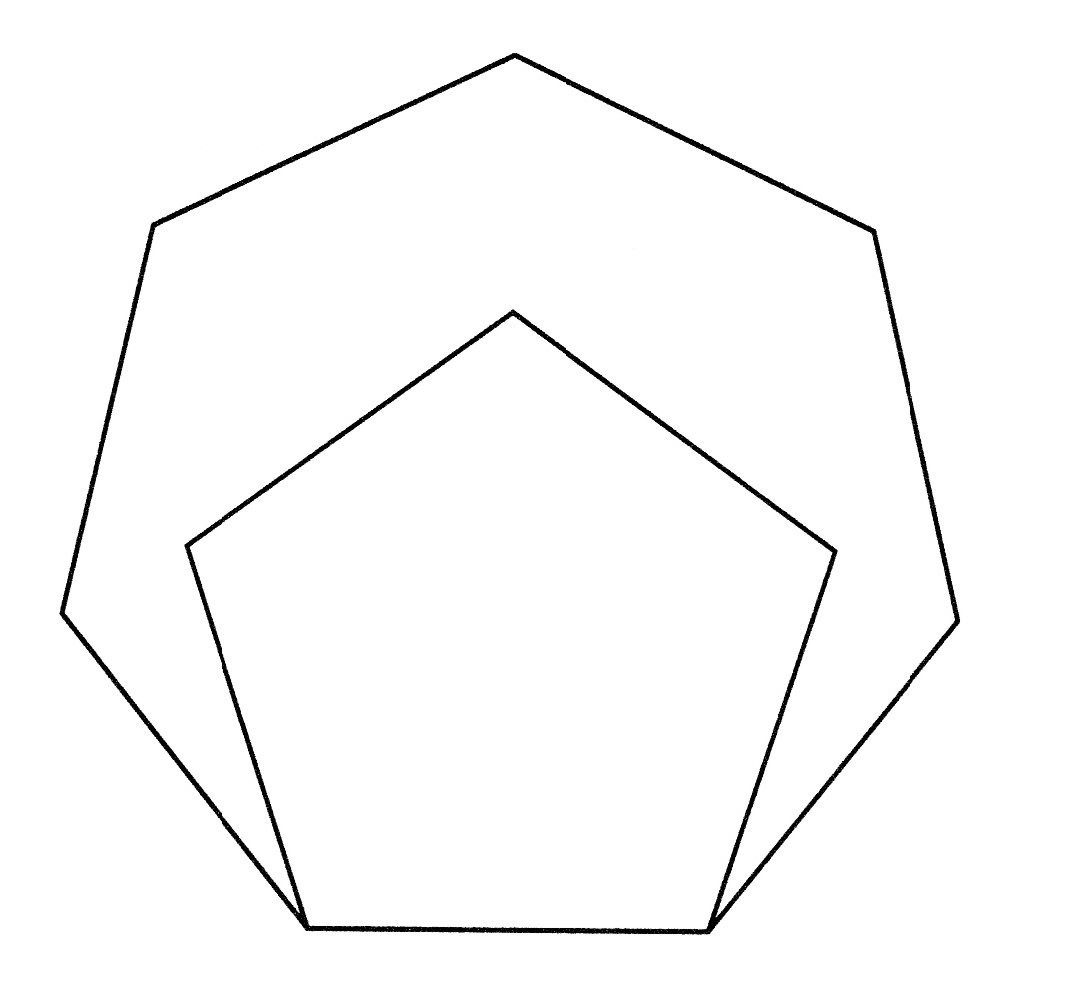
\includegraphics[scale=0.1]{Imatges/figuraS14-3.jpg}
\noindent
\textsf{\upshape
\begin{tabbing}
$|$ pica berthe $|$\\
berthe := Bot nou.\\
pica := Bot nou.\\
berthe poligon100: 5.\\
pica poligon100: 7.
\end{tabbing}}
\label{scr14-3}
\index{pentàgon, dibuixar amb el mètode poligon100:}
\index{variables!metodes@en mètodes|)}
\end{script}

\section{Experimentar amb múltiples arguments}
\index{metodes@mètodes!variables en|)}
\index{: (dos punts)!utilitzar en mètodes i paràmetres}
\index{dos punts (:)!utilitzar en mètodes i paràmetres}
\index{arguments!per a mètodes}
\index{metodes@mètodes!utilitzar arguments amb}
\index{metodes@mètodes!definir amb múltiples paràmetres}
Per quina raó hauríem de limitar-nos a polígons amb costats de mida 100? No seria millor tenir un mètode que dibuixés un polígon regular arbitrari, on tant el nombre de costats com la seva mida fossin determinats en el moment d'enviar el missatge? Per aconseguir això, caldrien dos paràmetres: \textsf{nombreDeCostats} i \textsf{midaCostat}. Així, com creem un mètode amb dos paràmetres? Podeu crear un mètode amb dos paràmetres escrivint el nom del mètode amb dos ``dos punts'' i posant un argument darrera de cada ``dos punts''.

\vspace*{1mm}
\noindent
\rule{\textwidth}{2pt}
\noindent
\textbf{Nota} Per definir un mètode amb múltiples paràmetres, acabeu cada paraula del nom del mètode (una paraula per a cada paràmetre) amb ``dos punts'', i poseu cada paràmetre darrera la seva paraula corresponent en el nom del mètode. El mètode anomenat \textsf{poligon:mida:} requereix dos arguments. La definició del mètode \textsf{poligon: nombreDeCostats mida: valorMida} defineix dos paràmetres, \textsf{nombreDeCostats} i \textsf{valorMida}. El primer paràmetre representa, com queda clar pel nom, el nombre de costats. El segon paràmetre està relacionat amb la mida del polígon. Ho explicarem tot seguit després de la definició del mètode.
\\
\noindent
\rule{\textwidth}{2pt}
\vspace*{1mm}

La definició del mètode \textsf{poligon:mida:} la teniu com a Mètode~\ref{met14-4}. Després de definir el mètode, podeu simplement enviar un missatge com ara \textsf{pica poligon: 7 mida: 100}. \index{poligon:mida: mètode, definir}

\newpage

\begin{metode}  
\textsf{\upshape
\begin{tabbing}
\hspace{5mm} \= \hspace{10mm} \= \kill
poligon: nombreDeCostats mida: valorMida\\
\> ``Dibuixa un polígon amb un nombre de costats i una mida per especificar''\\
\\
\> $|$ angle midaCostat $|$\\
\> angle := 360 / nombreDeCostats.\\
\> midaCostat := 4 * valorMida / nombreDeCostats. \\
\> nombreDeCostats vegadesRepetir:\\
\>\> [ self ves: midaCostat.\\
\>\> self giraEsquerra: angle ]\\
\end{tabbing}
}
\label{met14-4}
\index{valorMida paràmetre, exemple de}
\end{metode}

Us podeu preguntar per quina raó el paràmetre \textsf{valorMida} no especifica la mida del costat del polígon, i en canvi hem decidit definir la mida del costat (donada per la variable \textsf{midaCostat} en el mètode) com a \textsf{4 * valorMida / nombreDeCostats}. Per fer que tots els polígons amb el mateix \textsf{valorMida} tinguin aproximadament la mateixa mida, hem fet que tots els polígons tinguin el perímetre igual al perímetre d'un quadrat amb costats de mida \textsf{valorMida}. El perímetre d'aquest quadrat és \textsf{4 * valorMida}. El resultat és que fent que \textsf{midaCostat} sigui igual a \textsf{4 * valorMida / nombreDeCostats}, quan el robot dibuixa \textsf{nombreDeCostats} costats cada un de mida \textsf{midaCostat}, acaba fent un recorregut de distància igual al perímetre d'un quadrat amb costats de mida \textsf{valorMida}.
Així doncs, qualsevol polígon dibuixat amb \textsf{100} de segon argument tindrà un perímetre de valor \textsf{400} píxels, i tots els polígons ocuparan la mateixa fracció de la pantalla en ser dibuixats.\index{bucles imbricats, exemples de|seealso{bucles}}

Podeu pensar que el nom del paràmetre \textsf{nombreDeCostats} és una mica llarg i incòmode. Tot i així, és un bon nom per a un paràmetre, ja que pot ser comprès fàcilment per qualsevol persona que llegeixi el mètode. Com ja vam comentar en el capítol~\ref{cap9}, és molt important que el vostre codi sigui llegible, quasi bé com una narració, per a tothom. I això us inclou a vosaltres: el nom d'una variable o d'un paràmetre que no està clar us pot deixar aturats quan torneu al vostre codi al cap d'uns mesos d'haver-lo escrit.\index{parametres@paràmetres!donar nom als}

\begin{center}
\colorbox{black}{\makebox[\textwidth]{  \color{white} {\large {\bfseries Experiment 14-3}}}}
\end{center}
\index{rectangleAmplada:altura: mètode, definició}
{\small
\noindent
Definiu un mètode anomenat \textsf{rectangleAmplada:altura:} que dibuixa un rectangle amb la seva amplada i la seva altura com a arguments.}\\
\noindent
\rule{\textwidth}{3pt}
\newpage
\begin{center}
\colorbox{black}{\makebox[\textwidth]{  \color{white} {\large {\bfseries Experiment 14-4}}}}
\end{center}
\index{creuRecorregut1:recorregut2: mètode, definir}
{\small
\noindent
Modificant lleugerament el mètode \textsf{creu:} que vau escriure a l'Experiment 14-2, definiu un mètode \textsf{creuRecorregut1:recorregut2:}  que pugui dibuixar les creus estilitzades mostrades a la figura~\ref{fig1401}. Ordeneu els paràmetres de manera que una creu normal com la que dibuixaríeu amb \textsf{creu:} tingui el primer paràmetre igual al doble del segon, i per tant es pugui dibuixar amb expressions com \textsf{pica creuRecorregut1: 60 recorregut2: 30}.}\\
\noindent
\rule{\textwidth}{3pt}

\begin{figure}
\begin{center}
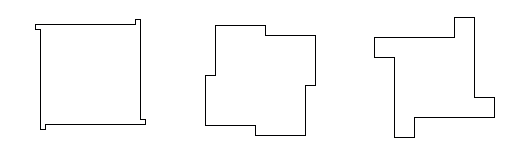
\includegraphics[scale=0.75]{Imatges/figura14-1.png}
\end{center}
\caption{Tres creus estilitzades generades pel mètode \textsf{\upshape creuRecorregut1:recorregut2:}. La creu de l'esquerra és el resultat de  \textsf{\upshape pica creuRecorregut1: 5 recorregut2: 50}; la creu del mig és el resultat de  \textsf{\upshape pica creuRecorregut1: 50 recorregut2: 5};  la creu de la dreta és el resultat de  \textsf{\upshape pica creuRecorregut1: 20 recorregut2: 40}.}
\label{fig1401}
\end{figure}

\section{Paràmetres i variables}
\index{variables!parametres@i paràmetres|(}
\index{parametres@paràmetres!variables@i variables|(}
Ara que ja heu practicat una mica, és el moment per investigar amb una mica de cura la diferència entre les variables normals i els paràmetres. Comparem l'\emph{script} i el mètode que ja hem definit per dibuixar un quadrat amb costats de mida arbitrària. Els hem tornat a reproduir com a \emph{Script}~\ref{scr14-4} i Mètode~\ref{met14-5}.

A l'\emph{Script}~\ref{scr14-4}, la variable \textsf{midaCostat} és declarada (línia 1), després rep un valor (línia 3), i finalment s'utilitza com a argument del mètode \textsf{ves:} (línia 5). \index{quadrat, \emph{script}, utilitzar variable amb}
\begin{script}  L'script del quadrat que utilitza una variable.
\textsf{\upshape
\begin{tabbing}
\hspace{7mm} \= \hspace{12mm} \= \kill
(1) \> $|$ pica midaCostat $|$\\
(2) \> pica := Bot nou.\\
(3) \> midaCostat := 10.\\
(4) \> 4 vegadesRepetir:\\
(5) \> \> [  pica ves: midaCostat.\\
(6) \> \> pica giraEsquerra: 90 ] \\
\end{tabbing}
}
\label{scr14-4}
\index{variables!utilitzar en l'\emph{script} del quadrat}
\end{script}

El Mètode~\ref{met14-5} mostra exemples de dues propietats dels paràmetres. Primer el paràmetre \textsf{midaCostat} és declarat posant-lo darrera de ``dos punts'' en el nom del mètode (línia 1). Segon, és utilitzat com a argument del missatge \textsf{ves:} (línia 5). Un paràmetre no s'inicialitza en la definició del mètode ja que sempre rep el seu valor de l'argument corresponent en qualsevol missatge que invoqui el mètode. Per exemple, quan el missatge \textsf{quadrat: 20} s'envia a \textsf{pica}, aleshores el paràmetre \textsf{midaCostat} del Mètode~\ref{met14-5} rep el valor \textsf{20}.\index{parametres@paràmetres!dibuixar quadrats amb} \index{parametres@paràmetres!propietats dels}

\begin{metode} El mètode que dibuixa quadrats utilitzant un paràmetre
\noindent
\textsf{\upshape
\begin{tabbing}
\hspace{7mm} \= \hspace{12mm} \= \kill
(1) \> quadrat: midaCostat\\
(2) \> ``Dibuixa un quadrat amb costats de la mida donada''\\
(3)\\
(4) \> 4 vegadesRepetir:\\
(5) \>\> [  self  ves: midaCostat.\\
(6) \>\> self giraEsquerra: 90  ]\\
\end{tabbing}
}
\label{met14-5}
\end{metode}

Així doncs, hi ha tres clares diferències entre paràmetres i variables: \index{: (dos punts)!utilitzar en paràmetres} \index{dos punts (:)!utilitzar en paràmetres} \index{parametres@paràmetres, canviar el valor dels} \index{parametres@paràmetres!declarar} 
\begin{itemize}
\item[] \textbf{Els paràmetres no es declaren explícitament.} Els paràmetres no es declaren entre barres verticals \textbar \hspace{2mm} \textbar , com cal fer amb les variables normals. Un paràmetre és declarat quan apareix darrera els ``dos punts'' a la primera línia de la definició d'un mètode.
\item[] \textbf{Als paràmetres no se'ls assigna valors.} Els paràmetres no es poden modificar de la mateixa manera que modifiquem les variables. No podem assignar nous valors als paràmetres dins del cos de la definició d'un mètode. Per exemple, l'expressió \textsf{midaCostat := 100} és impossible dins del Mètode~\ref{met14-5}. No podem modificar els valors d'un paràmetre ja que són una mena especial de variable. Són receptacles pels arguments utilitzats quan un missatge invoca el mètode corresponent, i els seus valors són assignats per Squeak quan un missatge és enviat, per tant no es poden assignar explícitament valors als paràmetres utilitzant \textsf{:=}.\index{parametres@paràmetres!no es pot assignar valors als}
\item[] \textbf{Inicialització de variables.} Les variables normals i els paràmetres obtenen els seus valors de maneres molt diferents. El valor d'una variable és canviat utilitzant una assignació explícita amb \textsf{:=}. El valor d'un paràmetre és assignat quan el mètode és invocat per un missatge. Per exemple, l'enviament de missatge \textsf{pica quadrat: 10} fa que el paràmetre \textsf{midaCostat} rebi el valor \textsf{10}. Per tant, un paràmetre és una variable, però d'un tipus especial el valor de la qual és assignat només en el moment en què un missatge és enviat i el mètode corresponent és executat.\index{parametres@paràmetres!variables@i variables|)} \index{variable, valor; canviar}\index{variables!parametres@i paràmetres|)}
\end{itemize}

\noindent
\rule{\textwidth}{2pt}
\noindent
\textbf{Nota} A part de les tres diferències entre paràmetres i variables normals, un paràmetre pot ser utilitzat dins el codi de la definició d'un mètode de la mateixa manera que qualsevol altra variable.
\\
\noindent
\rule{\textwidth}{2pt}

\section{Arguments i paràmetres}
\index{arguments!i paràmetres|(}
\index{parametres@paràmetres!arguments@i arguments|(}
Hem introduït els dos termes \emph{argument} i \emph{paràmetre} per a dues idees relacionades, tot i que diferents. Un argument és un objecte específic passat en un missatge. Un paràmetre és una variable receptacle utilitzada en la definició d'un mètode el valor de la qual és desconeguda quan el mètode és definit. Un paràmetre pren el seu valor de l'argument corresponent\footnote{Molts autors defineixen aquests termes de manera diferent. Alguns utilitzen ``paràmetre real'' pel que nosaltres anomenem ``argument'' i ``paràmetre formal'' pel que nosaltres anomenem ``paràmetre''. D'altres utilitzen els termes ``paràmetre'' i ``argument'' de manera intercanviable.}

A la figura~\ref{fig1402}, en el missatge \textsf{quadrat: 100}, el nombre \textsf{100} és l'argument del missatge. Quan el mètode \textsf{quadrat:} s'executa, el seu paràmetre \textsf{midaCostat} és col·locat a \textsf{100}, el valor de l'argument.
\begin{figure}[h]
\begin{center}
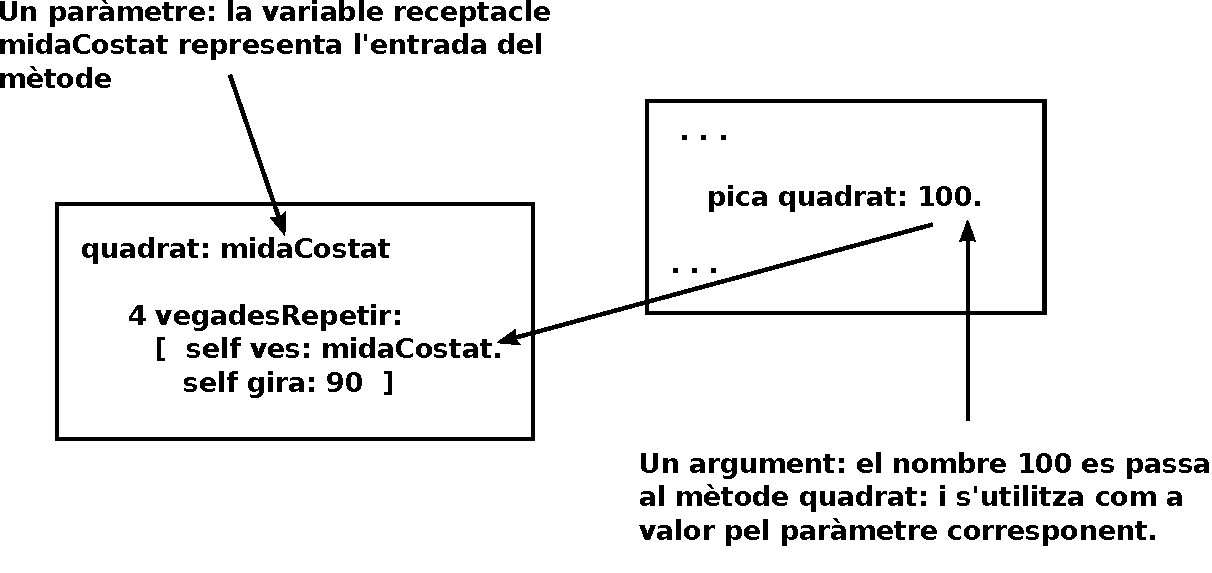
\includegraphics[scale=0.5]{Imatges/figura14-2.pdf}
\end{center}
\caption{La relació entre argument (un objecte) i paràmetre (una variable receptacle).}
\label{fig1402}
\end{figure}

Una altra manera d'entendre la diferència entre un argument i un paràmetre és que un paràmetre és un receptacle dins del mètode que representa una dada d'entrada pel mètode, mentre que un argument és el valor real que és passat com a entrada. Aquesta idea s'il·lustra a la figura~\ref{fig1403}.
\begin{figure}[h]
\begin{center}
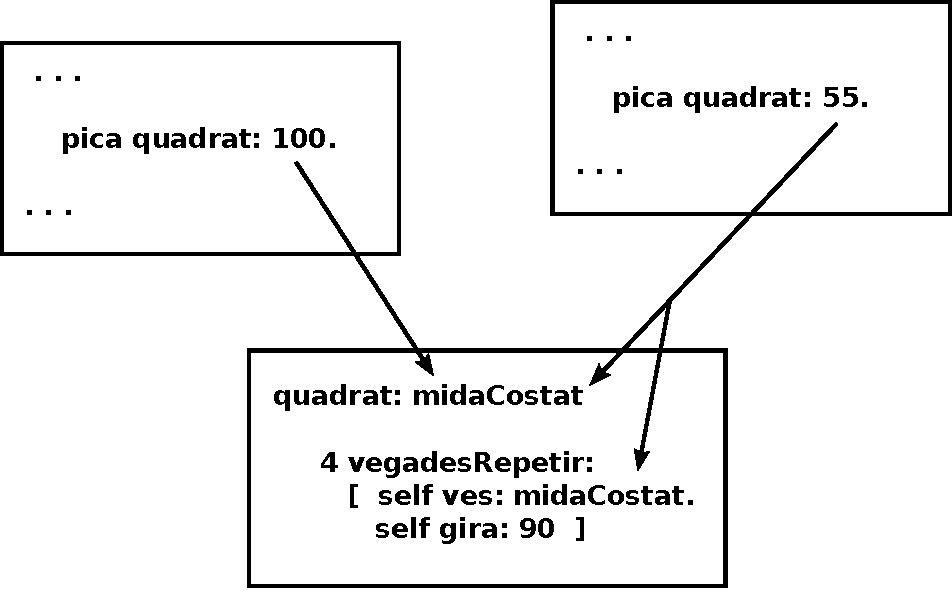
\includegraphics[scale=0.7]{Imatges/figura14-3.pdf}
\end{center}
\caption{El valor d'un argument queda lligat al paràmetre mentre el mètode s'executa.}
\label{fig1403}
\end{figure}

Fixeu-vos que un paràmetre es pot utilitzar també com a argument en altres enviaments de missatges. Per exemple, a la definició del mètode \textsf{quadrat:} (Mètode~\ref{met14-5}), el paràmetre \textsf{midaCostat} s'utilitza com a argument del missatge \textsf{ves: midaCostat}.

L'argument d'un missatge pot ser també una variable. Per exemple, a l'\emph{Script}~\ref{scr14-5}, que utilitza el mètode \textsf{quadrat:}, l'argument del primer missatge \textsf{quadrat:} és el valor de la variable \textsf{midaQuadrat}, que és \textsf{100}. L'argument del segon missatge \textsf{quadrat:} és el valor de l'expressió \textsf{midaQuadrat + 200}, que és \textsf{300}. El paràmetre \textsf{midaCostat} del mètode \textsf{quadrat:} pren el valor \textsf{100} al primer missatge \textsf{quadrat:}, i després el valor \textsf{300} del segon missatge \textsf{quadrat}. \index{variables!argument@com a argument}
\begin{script} Una variable com a argument.
\textsf{\upshape
\begin{tabbing}
\hspace{7mm} \= \hspace{12mm} \= \kill
$|$ pica midaQuadrat $|$\\
pica := Bot nou.\\
midaQuadrat := 100.\\
pica quadrat: midaQuadrat.\\
pica ves: 300.\\
pica quadrat: midaQuadrat.\\
\end{tabbing}
}
\label{scr14-5}
\end{script}

\subsection{Sobre l'execució dels mètodes}
\index{arguments!variables com a}
\index{metodes, exec@mètodes, execució|(}
En una primera lectura podeu saltar-vos aquesta secció, ja que entra en detalls que potser als programadors novells no els cal conèixer. L'hem escrit ja que volem respondre les preguntes dels lectors més curiosos, però ho podríem haver omès sense perdre continuitat.

Quan s'executa un mètode, es creen algunes variables. Aquestes variables són \textsf{self}, el receptor del missatge, i els paràmetres del mètode (que fan referència als arguments del mètode), com \textsf{midaCostat} a la figura~\ref{fig1404}, que mostra l'efecte d'enviar el missatge \textsf{quadrat: mida} a un robot a què ens referim amb la variable \textsf{pica}, on la variable \textsf{mida} fa referència al nombre \textsf{100}.
\begin{figure}[h]
\begin{center}
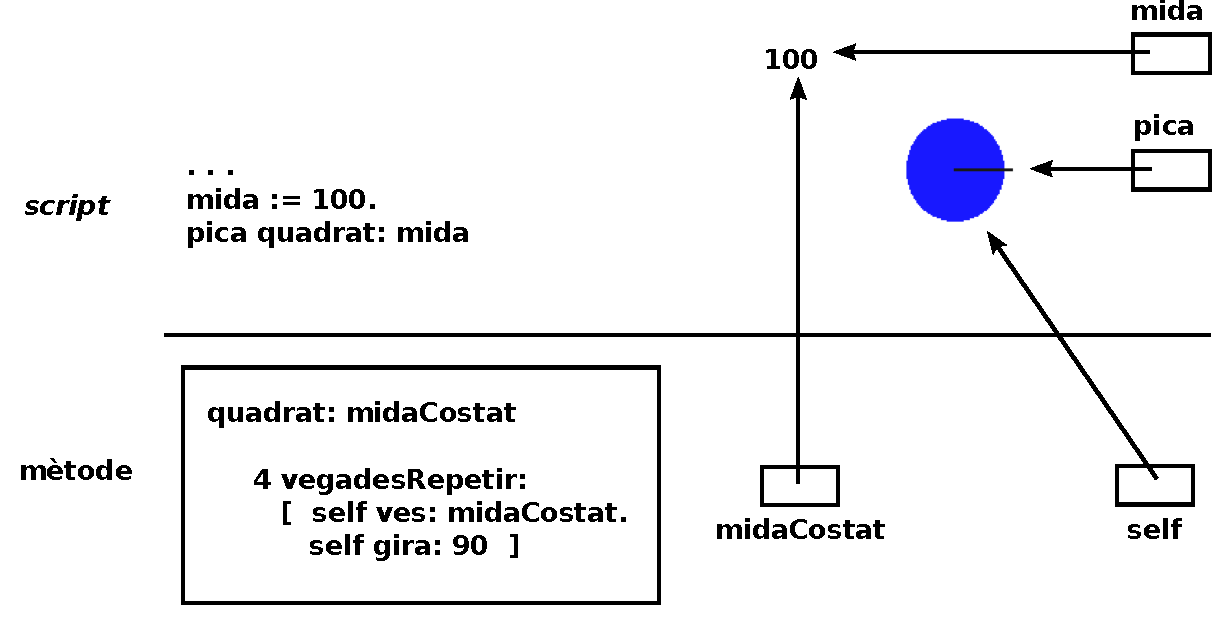
\includegraphics[scale=0.65]{Imatges/figura14-4.pdf}
\end{center}
\caption{Quan s'envia un missatge i s'executa un mètode, es creen noves variables que fan referència als arguments i al receptor del missatge.}
\label{fig1404}
\end{figure}

Quan el mètode \textsf{quadrat:} s'executa, la variable \textsf{self} fa referència al receptor del missatge, que en el nostre exemple és el robot apuntat per la variable \textsf{pica}; i el paràmetre \textsf{midaCostat} fa referència al valor de la variable \textsf{mida}, que aquí és el nombre \textsf{100}. El mateix procés succeeix per a cada enviament de missatge. Per exemple, l'execució de l'expressió \textsf{daly quadrat: 200} assigna a \textsf{self} el robot referenciat per la variable \textsf{daly} i assigna a \textsf{midaCostat} el nombre \textsf{200}.\index{quadrat: mètode!execució de}

Això pot semblar complicat, però no us heu d'amoïnar. Aquest són els passos amagats que Squeak realitza per assegurar-se que els paràmetres prenen els valors dels arguments dels missatges.\index{metodes@mètodes|seealso{compondre mètodes}} \index{self variable, relació amb els mètodes}

\section{Resum}
\index{metodes, exec@mètodes, execució|)}
\index{: (dos punts)!utilitzar en mètodes i múltiples arguments}
\index{dos punts (:)!utilitzar en mètodes i múltiples arguments}
\index{arguments!i paràmetres|)}
\index{parametres@paràmetres!arguments@i arguments|)}
\begin{itemize}
\item Un paràmetre és una mena especial de variable que actua com a receptacle per als arguments dels missatges. El paràmetre d'un mètode es declara tot just després dels ``dos punts'' en el nom del mètode, indicant la posició del paràmetre. Un paràmetre no s'ha de declarar com una variable, i no se li poden assignar valors dins del cos de la definició del mètode. Els paràmetres reben els seus valors dels arguments del missatge que invoca el mètode.
\item Per definir un mètode amb múltiples arguments, cal acabar cada paraula del nom del mètode amb ``dos punts'', i col·locar cada paràmetre després de la corresponent paraula del nom del mètode. Per exemple, el mètode anomenat \textsf{poligon:mida:} requereix dos arguments. La definició del mètode \textsf{poligon: nombreDeCostats mida: valorMida} defineix dos paràmetres, \textsf{nombreDeCostats} i \textsf{valorMida}.
\end{itemize}

\chapter{Errors i depuració} 
\label{cap15}

Ara que ja sabeu com definir mètodes que criden altres mètodes, podeu escriure programes més i més complexos. Més tard o més d'hora cometreu algun error i no aconseguireu trobar què és el que està malament.
Els errors en els programes d'ordinador s'anomenen \emph{bugs}\footnote{\emph{Nota del Traductor:} D'on ve l'expressió \emph{debugging} que aquí hem traduït com a ``depuració'', seguint els consells de softcatalà.}, i us ensenyarem com utilitzar una eina molt potent que us ajudarà a trobar aquests errors, i corregir-los: el depurador d'Squeak (l'\emph{Squeak debugger}\footnote{\emph{Nota del Traductor:} Com ja sabeu, el depurador d'Squeak és una eina de l'entorn general, i no pròpiament de l'entorn BotsInc, per tant no ha estat traduïda, 
tal i com hem fet amb algunes eines que ja hem trobat en aquest llibre.}).

Un \emph{depurador} és una eina que mostra l'execució d'un programa. Us deixa inspeccionar i canviar els valors de les variables i editar els mètodes d'un programa. En aquest capítol us ensenyarem alguns exemples típics d'errors i us explicarem què és el depurador i com utilitzar-lo. Començarem presentant alguns errors comuns amb variables. Després us mostrarem com utilitzar el depurador per identificar i arreglar altres tipus de problemes. \index{depurador (\emph{debugger})!definició del}

\section{El valor per defecte d'una variable}
\index{nil valor, significat de|(}
\index{variables!valor per defecte de|(}
\index{valors!representar amb nil|(}
Les variables són molt útils per programar, però requereixen que hi poseu una mica d'atenció. Per exemple, podeu introduir
fàcilment un error en un programa utilitzant una variable que no ha estat declarada o a la qual s'han assignat valors incorrectes. Fins i tot els programadors amb experiència cometen errors. Aquests, però, saben com trobar-los i eliminar-los. Squeak us ajuda una mica comprovant, per exemple, si les variables que utilitzeu han estat declarades. Aquests errors estructurals, o \emph{sintàctics}, són fàcils de localitzar, i Squeak els localitzarà. Tot i així, Squeak no té cap manera de detectar errors \emph{lògics}, com ara assignar a una variable el valor 1000 quan li hauríeu d'haver assignat el valor 100. Aquests errors els haureu de trobar vosaltres mateixos, i utilizar un depurador us pot ajudar a entendre, localitzar i eliminar els vostres errors.

Primer, experimentem una mica. Escriviu, seleccioneu i demaneu el resultat de l'\emph{Script}~\ref{scr15-1}, que declara la variable \textsf{mida} i prova de fer-la servir abans de ser inicialitzada. Hauríeu d'obtenir la figura~\ref{fig1501}, que mostra com Squeak us avisa quan una variable no ha estat inicialitzada. Si trieu l'opció \textbf{si} quan us pregunti, hauríeu d'obtenir \textsf{nil} escrit com veieu a la dreta de la figura~\ref{fig1501}. El valor \textsf{nil} que tot just heu obtingut és un objecte especial assignat a qualsevol variable declarada. Començarem per mirar el valor per defecte d'una variable.
\begin{figure}[h]
\begin{center}
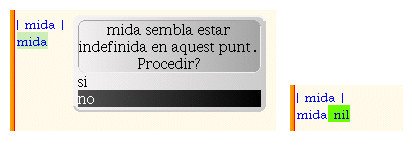
\includegraphics[scale=3.0]{Imatges/figura15-1.png}
\end{center}
\caption{\emph{Esquerra:} Squeak us avisa quan proveu d'utilitzar una variable que no ha estat inicialitzada.
\emph{Dreta:} El valor \textsf{\upshape nil} s'escriu si decidiu procedir responent \textsf{\upshape si}.}
\label{fig1501}
\end{figure}

\begin{script} Provar d'utilitzar una variable abans d'inicialitzar-la.
\textsf{\upshape
\begin{tabbing}
\hspace{7mm} \= \hspace{12mm} \= \kill
$|$ mida $|$\\
mida\\
\end{tabbing}
}
\label{scr15-1}
\index{mida, variable; declarar}
\end{script}

La raó de la queixa d'Squeak quan utilitzeu una variable que no ha estat inicialitzada és que si no inicialitzeu una o més variables, és pràcticament segur que el vostre programa és incorrecte, ja que estareu utilitzant una variable que té un valor incorrecte o fins i tot cap valor. El valor de les variables a Smalltalk és per defecte l'objecte \textsf{nil}, que representa un valor indefinit. Tot i que \textsf{nil} és un objecte com qualsevol altre, no entén gaires missatges. En particular, no entén cap dels missatges que s'envien als objectes nombre o als objectes robot. Per tant, obtindreu un error en provar d'enviar un d'aquests missatges a l'objecte \textsf{nil}. L'objecte \textsf{nil} és important per determinar si una variable té o no un valor assignat.

\newpage

\noindent
\rule{\textwidth}{2pt}
\noindent
\textbf{Important!} A Smalltalk, el valor d'una variable no inicialitzada és per defecte l'objecte \textsf{nil}, que s'utilitza per representar un valor indefinit.\\
\noindent
\rule{\textwidth}{2pt}
\vspace*{1mm}

L'error que succeeix mentre provem d'executar l'\emph{Script}~\ref{scr15-1} genera el missatge que podem veure a la figura~\ref{fig1501}. Normalment, és suficient respondre \textbf{no} i tornar a l'\emph{script} per inicialitzar la variable. Tot i així, malgrat Squeak és capaç d'analitzar els \emph{scripts} i trobar aquests errors estructurals, no pot detectar, abans d'executar un \emph{script}, si heu utilitzat una valor  \emph{no vàlid}. En aquest cas, Squeak obre un \emph{depurador} (\emph{debugger} en anglès) que podeu utilitzar per accedir l'estat de l'execució, que inclou el receptor del missatge, el missatge mateix, les variables involucrades, etc. Això és el que ara us explicarem. \index{nil valor, significat de|)} \index{valors!representar amb nil|)} \index{variables!valor per defecte de|)}

\section{Examinar l'execució d'un missatge}

Per si de cas us heu oblidat de les definicions dels mètodes \textsf{patro} i \textsf{patro4}, els hem tornat a escriure aquí (Mètodes~\ref{met15-1} i~\ref{met15-2}). El que és important és adonar-se que el mètode \textsf{patro4} utilitza el mètode \textsf{patro}, mentre que el mètode \textsf{patro} invoca els mètodes \textsf{ves:} i \textsf{giraDreta:}.\index{missatge, examinar l'execució del|(} \index{patro, mètode!definir} \index{patro4, mètode!definir}
\begin{metode} 
\noindent
\textsf{\upshape
\begin{tabbing}
\hspace{5mm} \= \kill
{\bfseries patro}\\
\> ``dibuixa un patró''\\
\\
\> self ves: 100.\\
\> self giraDreta: 90.\\
\> self ves: 100.\\
\> self giraDreta: 90.\\
\> self ves: 50.\\
\> self giraDreta: 90.\\
\> self ves: 50.\\
\> self giraDreta: 90.\\
\> self ves: 100.\\
\> self giraDreta: 90.\\
\> self ves: 25.\\
\> self giraDreta: 90.\\
\> self ves: 25.\\
\> self giraDreta: 90.\\
\> self ves: 50.
\end{tabbing}
}
\label{met15-1}
\end{metode}

\begin{metode} 
\noindent
\textsf{\upshape
\begin{tabbing}
\hspace{5mm} \= \hspace{10mm} \= \kill
{\bfseries patro4}\\
\> ``dibuixa quatre patrons''\\
\\
\> 4 vegadesRepetir: [ self patro ]
\end{tabbing}
}
\label{met15-2}
\end{metode}

Després de definir aquests mètodes, si Squeak executa l'expressió \textsf{Bot nou patro4}, diversos missatges són invocats en una reacció en cadena el resultat final de la qual és que el robot dibuixa quatre patrons a la pantalla. Examinem aquesta cadena de missatges: Primer, \textsf{Bot nou} crea un robot nou, al que el missatge \textsf{patro4} s'envia. Com a resultat, el mètode \textsf{patro4} és executat. Aquesta execució envia el missatge \textsf{vegadesRepetir:}, el qual envia el missatge \textsf{patro}. L'execució del mètode \textsf{patro} envia diversos missatges, en concret \textsf{ves:} i \textsf{giraDreta:}. En l'argot dels llenguatges de programació, aquesta cadena de missatges s'anomena la pila d'execució: la pila conté tots els mètodes executats com a reacció a un missatge inicial i la cadena de missatges que aquests mètodes han executat, després tots els mètodes executats com a reacció a aquest segon conjunt de missatges i la cadena de missatges que aquests mètdes han executat i així successivament fins que no queden més missatges. \index{negreta (tipus de lletra), significat de |(}

Una representació possible la podeu veure a la figura~\ref{fig1502}, on el darrer mètode executat és a sobre de tot, i així successivament cap avall. Un mètode que crida un altre mètode apareix sota el mètode cridat. La part de cada expressió que porta a la invocació del mètode sobre seu apareix en negreta. Mirem què passa detalladament:
\begin{itemize}
\item[\textbf{1.}] A la capsa de baix de tot, el missatge \textsf{nou} és enviat a la classe \textsf{Bot}, que crea un robot nou.
\item[\textbf{2.}] El missatge \textsf{patro4} és enviat al robot creat.
\item[\textbf{3.}] L'execució del mètode \textsf{patro4} envia el missatge \textsf{vegadesRepetir: [ self patro ]}. El missatge \textsf{vegadesRepetir:} està en negreta, ja que és el primer en ser enviat.
\item[\textbf{4.}] L'execució del mètode \textsf{vegadesRepetir:} porta a l'execució del bloc. Aquesta es fa mitjançant l'enviament el missatge \textsf{value} a l'argument del missatge \textsf{vegadesRepetir:}.
\item[\textbf{5.}] Dins del mètode \textsf{patro4}, el missatge \textsf{patro} és enviat pel mètode \textsf{vegadesRepetir:} com a resultat de l'execució del bloc.
\item[\textbf{6.}] El procés continua de manera similar, amb els missatges del mètode \textsf{patro} executant-se un darrera l'altre.
\end{itemize}

\begin{figure}
\begin{center}
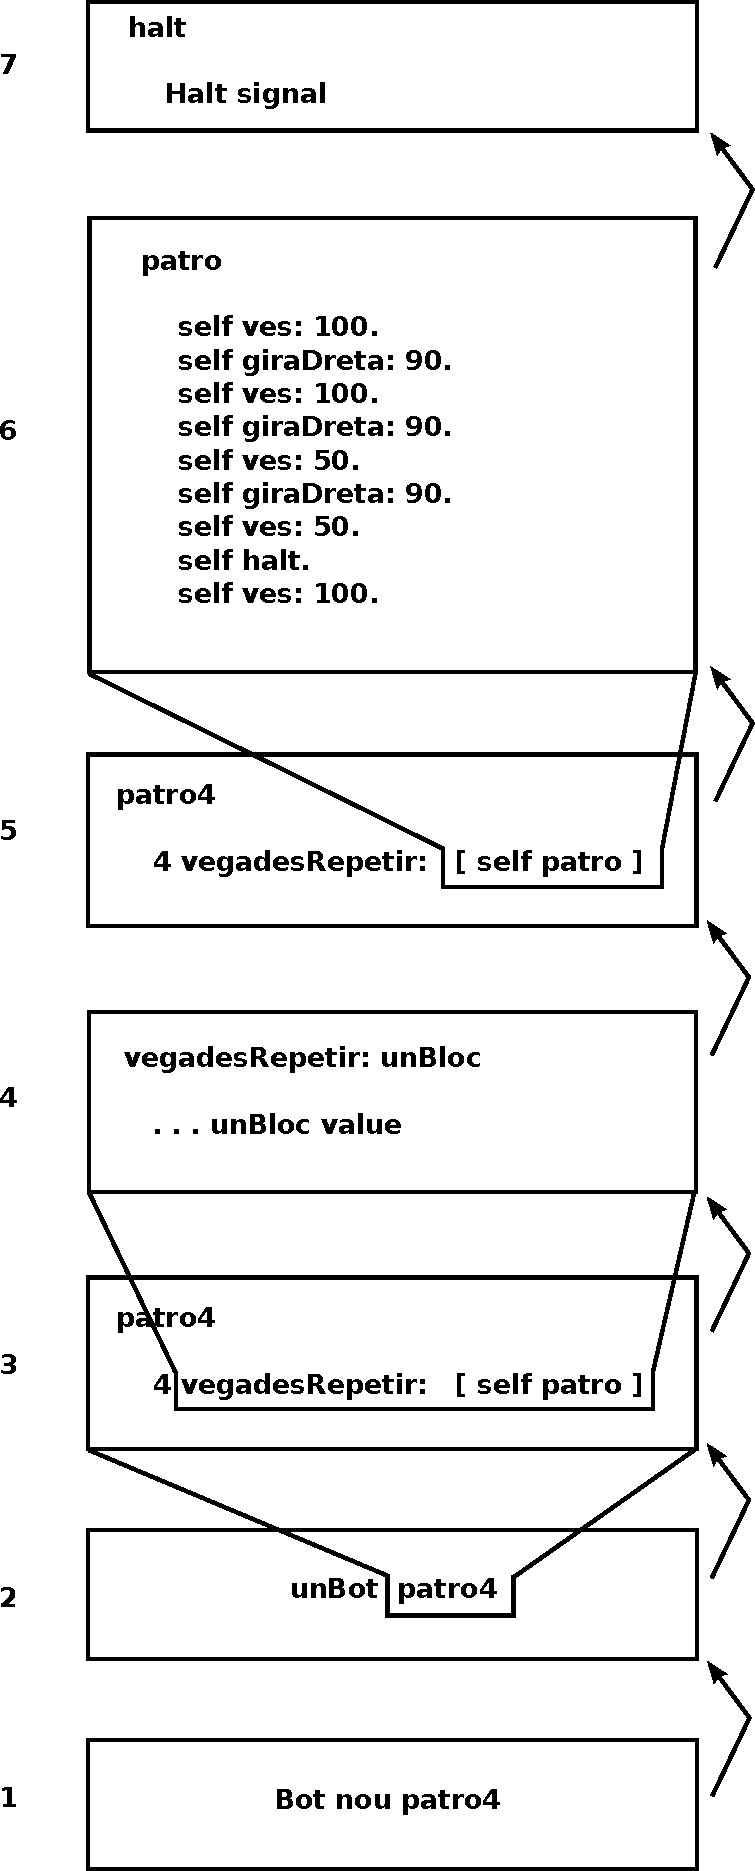
\includegraphics[scale=0.5]{Imatges/figura15-2.pdf}
\end{center}
\caption{La pila d'execució, que conté tots els missatges i els mètodes invocats com a resultat de l'execució de \textsf{\upshape Bot nou patro4}.}
\label{fig1502}
\end{figure}

La figura~\ref{fig1502} conté una altra capsa que explicarem de seguida. El que hauríeu d'entendre ara és que un mètode crida un altre i que el mètode cridat és col·locat a la pila a sobre del mètode que el crida.\index{negreta (tipus de lletra), significat de |)} \index{Bot nou patro4, execució de} \index{pila d'execució, exemple de} \index{missatge, examinar l'execució del|)}

\section{Una primera ullada al depurador}
\index{depurador (\emph{debugger})!invocar|(}
\index{expressions!self halt|(}
\index{self halt expressió, obrir el depurador amb|(}
La figura~\ref{fig1502} mostra la manera en la que podeu imaginar la seqüència de missatges enviats i mètodes executats com a resultat de l'execució d'un missatge. El depurador d'Squeak us deixa veure, explorar i canviar la cadena de missatges. El depurador s'invoca automàticament quan un objecte no entén un missatge que li han enviat, com discutirem més tard, però també podeu invocar-lo explícitament amb l'expressió \textsf{self halt} dins del cos d'un mètode. Introduir aquesta expressió és útil quan voleu entendre com s'executa una expressió o localitzar un error en un programa.\index{receptors dels missatges|see{missatges}}
\index{missatges|seealso{binaris, missatges; cascades; paraula-clau, missatges; ordre d'execució; unaris, missatges}}
\noindent
\rule{\textwidth}{2pt}
\noindent
\textbf{Important!} El depurador d'Squeak és una eina que us permet explorar una seqüència de mètodes executats. Utilitzant el depurador, podeu conèixer els valors dels arguments dels mètodes, modificar la definició d'un mètode, canviar i veure els valors de variables i arguments, i continuar l'execució.\\
\noindent
\rule{\textwidth}{2pt}
\vspace*{1mm}

Per obrir el depurador, afegiu l'expressió \textsf{self halt} dins del mètode \textsf{patro}, com veieu al Mètode~\ref{met15-3}. Després executeu l'expressió \textsf{Bot nou patro4}. Hauríeu d'obtenir la situació mostrada a la figura~\ref{fig1503}. Primer es crea un robot nou, després comença a dibuixar el primer patró, i després de dibuixar quatre línies s'atura i apareix una finestra oferint-vos la possibilitat d'obrir el depurador.

\begin{figure}
\begin{center}
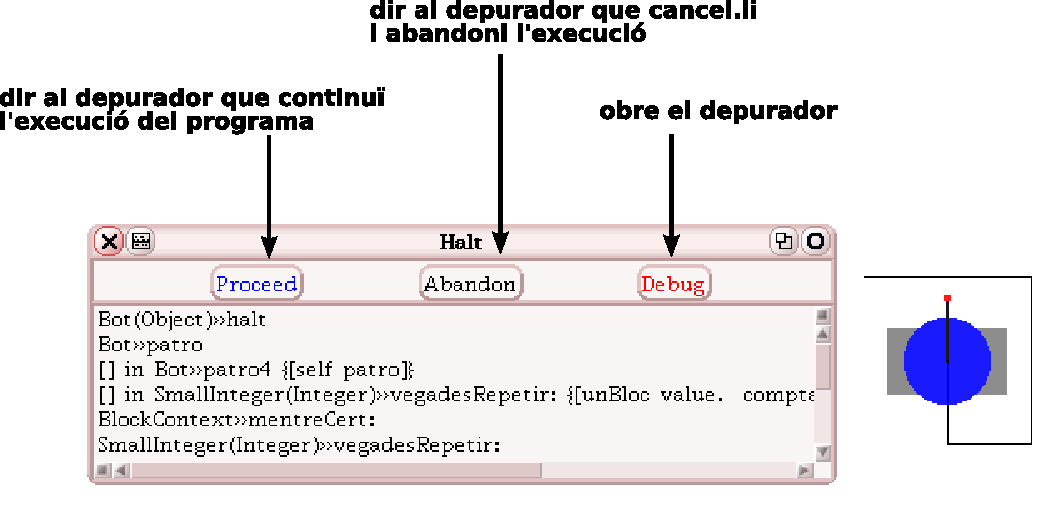
\includegraphics[scale=0.65]{Imatges/figura15-3.pdf}
\end{center}
\caption{El robot comença a dibuixar el començament del primer patró, però després de dibuixar quatre línies, s'atura i podeu obrir el depurador.}
\label{fig1503}
\end{figure}
\newpage
\begin{metode} Introduir l'expressió \textsf{{\upshape self halt}} dins d'un mètode obre una finestra que us ofereix la possibilitat d'obrir el depurador.
\noindent
\textsf{\upshape
\begin{tabbing}
\hspace{5mm} \= \kill
{\bfseries patro}\\
\> ``dibuixa un patró''\\
\\
\> self ves: 100.\\
\> self giraDreta: 90.\\
\> self ves: 100.\\
\> self giraDreta: 90.\\
\> self ves: 50.\\
\> self giraDreta: 90.\\
\> self ves: 50.\\
\> {\bfseries self halt.}\\
\> self giraDreta: 90.\\
\> self ves: 100.\\
\> self giraDreta: 90.\\
\> self ves: 25.\\
\> self giraDreta: 90.\\
\> self ves: 25.\\
\> self giraDreta: 90.\\
\> self ves: 50.
\end{tabbing}
}
\label{met15-3}
\end{metode}

\noindent
\rule{\textwidth}{2pt}
\noindent
\textbf{Important!} Per invocar el depurador, inseriu l'expressió \textsf{self halt} dins del cos d'un mètode. L'execució de l'expressió \textsf{self halt} obre una finestra oferint-vos la possibilitat d'obrir el depuador.\\
\noindent
\rule{\textwidth}{2pt}
\vspace*{1mm}

La finestra del depurador mostrada a la figura~\ref{fig1503} ofereix tres botons: \textbf{Proceed} (Procedir), \textbf{Abandon} (Abandonar), i \textbf{Debug} (Depurar). 
\index{expressions!self halt|)}
\index{Abandon, botó; a la finestra del depurador, efecte}
\index{Debug, botó; a la finestra del depurador, efecte}
\index{depurador (\emph{debugger})!invocar|)} \index{self halt expressió, obrir el depurador amb|)}
\begin{itemize}
\item[] \textbf{Proceed.} Aquest botó li diu al depurador que continuï l'execució del mètode, ignorant el missatge \textsf{self halt}. Fixeu-vos que és possible procedir només si heu obert el depurador utilitzant \textsf{self halt}. Si teniu un error de debó que obre el depurador, utilitzar \textbf{Proceed} no és de cap ajuda, ja que Squeak no pot continuar.\index{Proceed, botó; utilitzar al depurador}
\item[] \textbf{Abandon.} Aquest botó li diu al depurador que es tanqui, i l'execució del mètode és aturada.
\item[] \textbf{Debug.} Aquest botó li diu al depurador que s'obri. A la figura~\ref{fig1504} podeu veure una finestra oberta del depurador.
\end{itemize}

\begin{figure}[h]
\begin{center}
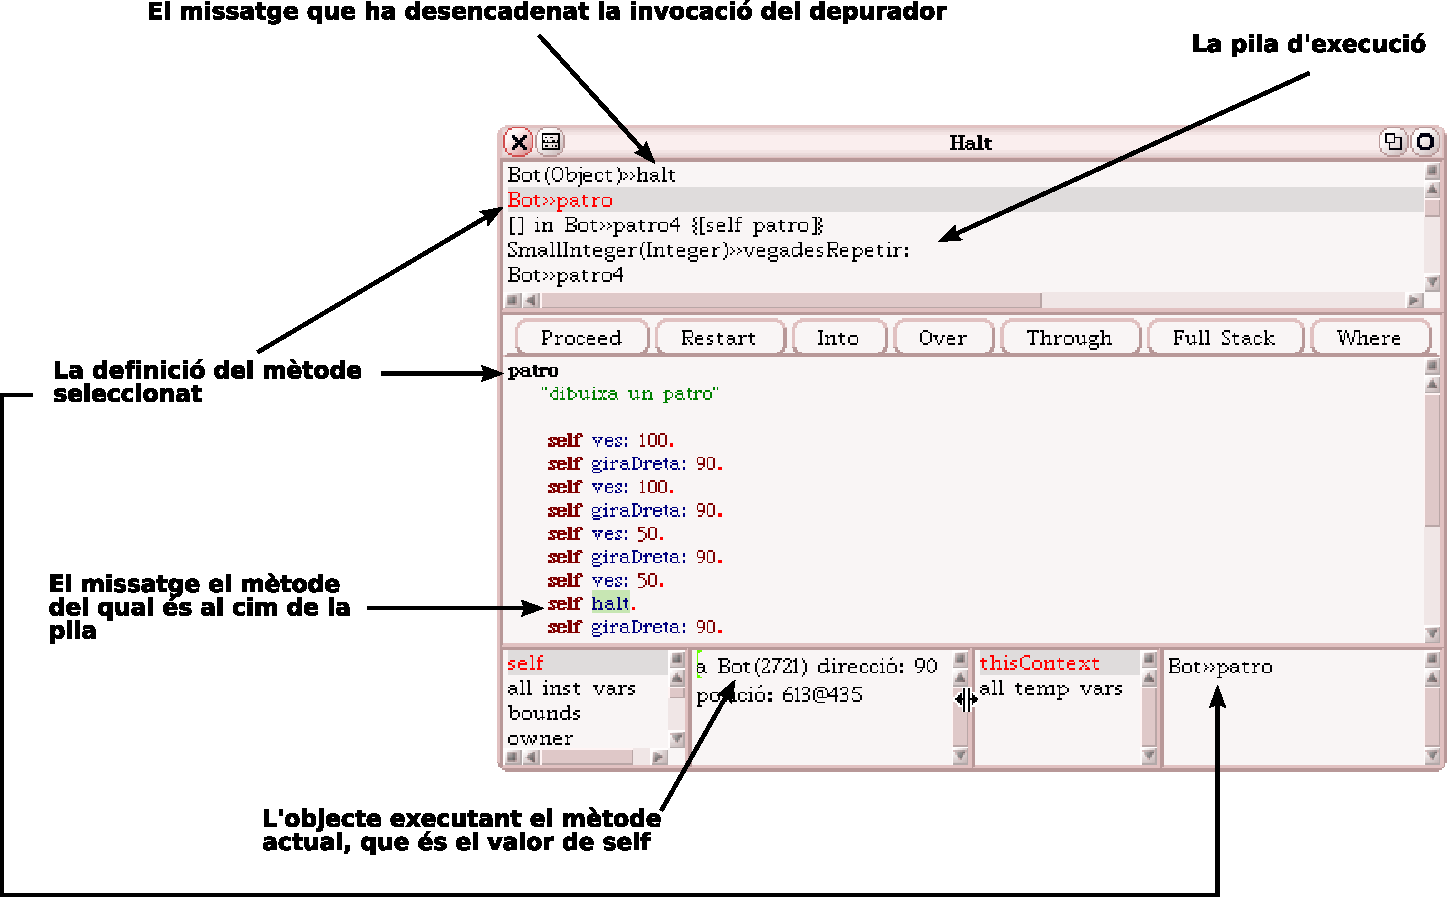
\includegraphics[scale=0.525]{Imatges/figura15-4.pdf}
\end{center}
\caption{La finestra del depurador. El mètode \textsf{\upshape patro} està seleccionat.}
\label{fig1504}
\end{figure}

Si premeu \textbf{Debug} i seleccioneu la segona línia de la subfinestra de dalt de tot, obteniu la finestra mostrada a la figura~\ref{fig1504}. Com podeu veure, el depurador es composa de diverses subfinestres. La subfinestra de dalt de tot representa la pila d'execució, que ja vau veure esquematitzada a la figura~\ref{fig1502}. Tots els missatges que han estat enviats fins l'\textsf{halt} són mostrats, amb els missatges més recents al cim. El missatge més recent és, naturalment, \textsf{halt}, i per tant és al cim de la pila. Aquest és el missatge que ha desencadenat l'obertura de la capsa de diàleg mostrada a la figura~\ref{fig1503}.\index{depurador, obrir la finestra del}

Seleccionar una de les línies de la subfinestra superior fa que la definició del mètode apareixi a la subfinestra del mig. A  la figura~\ref{fig1504} es veu que hem seleccionat a la pila el mètode \textsf{patro}, i la seva definició la podeu veure a la segona subfinestra gran. L'objecte que ha rebut el missatge \textsf{patro} (que és l'objecte al que la variable \textsf{self} es refereix) i que l'ha executat és mostrat a la subfinestra de baix de tot.\index{patro, mètode!seleccionar a la finestra del depurador}

Al cos del mètode seleccionat a la pila, que en el nostre exemple és \textsf{patro}, el depurador ressalta en verd el mètode l'execució del qual està ara mateix aturada, i que, a la pila, està al damunt del mètode seleccionat. Aquí \textsf{self halt} està aturat, i està al damunt de \textsf{patro} a la pila. Podeu també fixar-vos que totes les expressions per sobre de \textsf{self halt} dins el cos del mètode ja han estat executades, mentre que les expressions de sota no ho han estat encara. En aquest exemple, 
\textsf{self ves: 100. self giraDreta: 90. self ves: 100. self giraDreta: 90. self ves: 50. self giraDreta: 90. self ves: 50.}
ja han estat executades.

Si seleccioneu la tercera línia de la subfinestra superior, és a dir, el mètode \textsf{patro4}, veureu, com es mostra a l'esquerra de la figura~\ref{fig1505}, que la pila de l'execució del mètode \textsf{patro4} a dalt, està relacionada amb l'execució de l'expressió \textsf{self patro} del mètode \textsf{patro4}. Ara, si seleccioneu la cinquena línia, veieu un altre cop el mètode \textsf{patro4}, però ara abans que s'executi el bucle \textsf{vegadesRepetir:}. \index{patro4, mètode!seleccionar dins del depurador}

Si seleccioneu la quarta línia, com podeu veure a la figura~\ref{fig1505}, veieu la definició del mètode \textsf{vegadesRepetir:}. Podeu veure a la subfinestra superior que l'objecte que rep el missatge \textsf{vegadesRepetir:} no  és un robot, sinó un nombre enter. En el nostre exemple, el receptor del bucle és l'objecte \textsf{4}, a l'expressió \textsf{4 vegadesRepetir: [ self patro ]}. Això significa que dins d'aquest mètode, la variable \textsf{self} està lligada a un objecte enter. Això no és inusual, ja que la variable \textsf{self} \emph{sempre} representa l'objecte que ha rebut el missatge actual. \index{vegadesRepetir: mètode!mostrar en el depurador} 
\begin{figure}[h]
\begin{center}
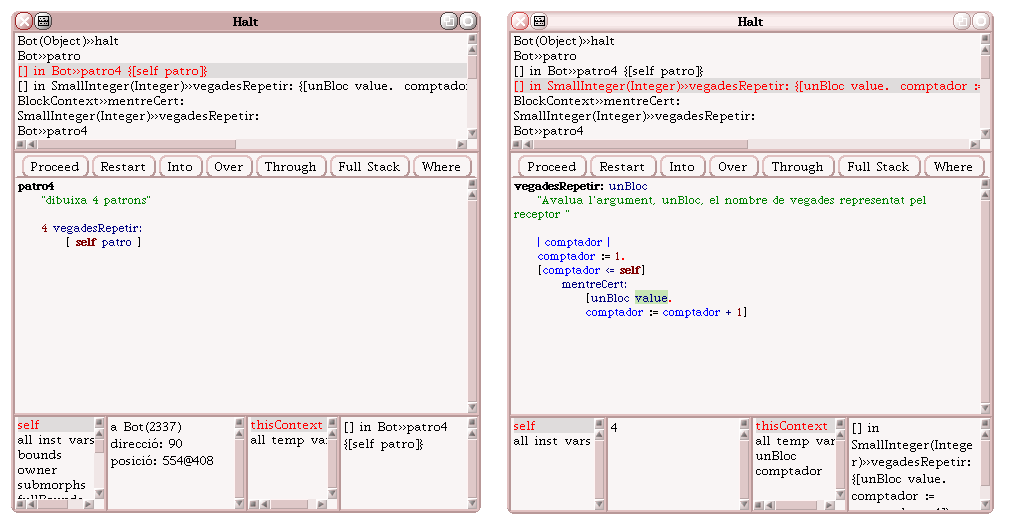
\includegraphics[scale=0.4]{Imatges/figura15-5.png}
\end{center}
\caption{\emph{Esquerra:} El mètode \textsf{\upshape patro4} s'ha seleccionat.
\emph{Dreta:} El mètode \textsf{\upshape vegadesRepetir:} s'ha seleccionat.}
\label{fig1505}
\end{figure}

\section{Anar pas a pas per la pila}
\index{pila, depurador; anar pas a pas per la}
Amb el depurador d'Squeak no només podeu explorar la pila i identificar els receptors de diversos missatges, sinó que també us deixa executar un mètode pas a pas. Podeu dir-li al depurador de realitzar diferentes accions utilitzant els botons que hi ha entre la primera i la segona subfinestra. Aquí teniu una descripció de les més útils, ordenades de dreta a esquerra. \index{depurador (\emph{debugger})|seealso{errors; errors de programa}} \index{depurador (\emph{debugger})!tancar}
\begin{itemize}
\item[] \textbf{Proceed.} Prémer aquest botó té el mateix efecte que prémer el botó \textbf{Proceed} a la capsa de diàleg de la figura~\ref{fig1503}. El depurador es tanca i l'execució del mètode continua si és possible.\index{Proceed, botó; utilitzar al depurador}
\item[] \textbf{Restart.} Podeu demanar-li al depurador que torni a començar l'execució del mètode actual. Fixeu-vos que de vegades fer això pot portar problemes, ja que podeu estar modificant el mateix objecte dues vegades, obtenint resultats inesperats o fins i tot errors.\index{Restart, botó; utilitzar al depurador}
\item[] \textbf{Into.} Aquest botó i el proper són els botons més útils del depurador, i els que s'utilitzen més sovint. Prémer aquest botó us porta dins del mètode seleccionat sense executar-lo. És a dir, podeu examinar el codi del mètode seleccionat, tal i com apareix a la segona subfinestra del depurador, sense que tingui lloc cap execució del mètode. Veieu la figura~\ref{fig1506} com a exemple, en què el mètode \textsf{giraDreta:} del mètode \textsf{patro} s'ha seleccionat i es pot examinar.\index{Into, botó; utilitzar al depurador}
\begin{figure}[h!]
\begin{center}
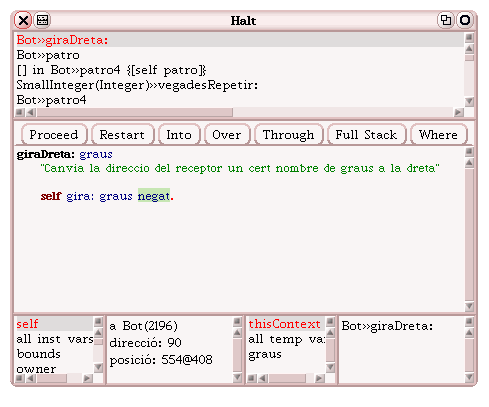
\includegraphics[scale=0.4]{Imatges/figura15-6.png}
\end{center}
\caption{Entrant dins del mètode \textsf{\upshape giraDreta:}.}
\label{fig1506}
\end{figure}
\item[] \textbf{Over.} Prémer aquest botó us permet executar el missatge seleccionat sense examinar-lo. Només s'executa l'expressió i s'atura. Veieu la figura~\ref{fig1507}. En aquesta figura hem \emph{examinat} el mètode \textsf{patro}, i després he \emph{executat} algunes expressions dins del mètode \textsf{patro}. Podeu veure a la figura que ens hem aturat a l'expressió \textsf{ves: 25}. Encara som dins del mètode \textsf{patro} ja que no hem volgut examinar cap de les expressions que composen \textsf{patro}. A mida que es van executant les expressions, hauríeu de veure el robot realitzant cada acció, una darrera l'altra. Fixeu-vos que quan sigueu al final del mètode, havent executat totes les expressions, el botó \textbf{Over} us retorna al mètode que ha invocat el mètode actual, i us moveu cap avall a la pila. Per exemple, després d'acabar d'executar \textsf{patro}, tornareu a \textsf{patro4}.\index{Over, botó; utilitzar al depurador} \index{missatges!executar}\index{metodes@mètodes!depurar}
\begin{figure}[h!]
\begin{center}
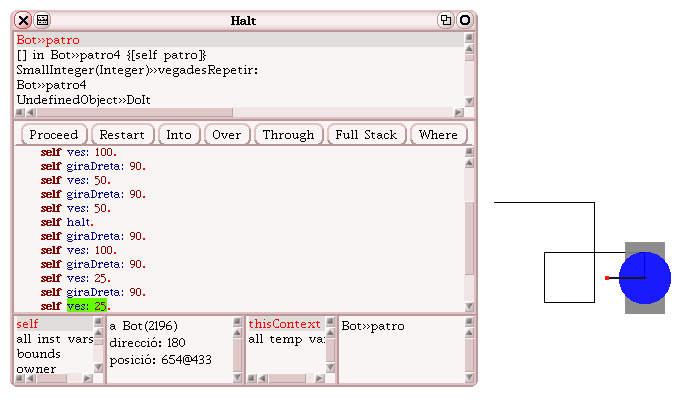
\includegraphics[scale=0.5]{Imatges/figura15-7.png}
\end{center}
\index{patro, mètode!examinar}
\caption{Examinant el mètode \textsf{\upshape patro} i executant cada missatge, podeu veure com el robot executa cada expressió una a una.}
\label{fig1507}
\end{figure}
\end{itemize}

Quan premeu el botó \textbf{Into}, esteu demanant al depurador d'\emph{examinar} el mètode sense executar-lo. Per exemple, si l'expressió seleccionada dins el mètode \textsf{patro} és \textsf{self giraDreta: 90}, podeu simplement executar l'expressió prement el botó \textbf{Over} o podeu prémer el botó \textbf{Into}, que li diu al depurador d'anar dins del mètode \textsf{giraDreta:}, aturant-se a la primera expressió, com es mostra a la figura~\ref{fig1506}, on el primer missatge a enviar és el missatge \textsf{negat}. Aquí també teniu l'opció d'examinar l'expressió \textsf{negat} o executar-la. I un cop més, quan arribeu al final del mètode, retorneu al mètode que crida el mètode on sou ara. També podeu veure els valors dels arguments passats al mètode seleccionant el nom de l'argument al cos del mètode i triant \textbf{escriu-ho} (figura~\ref{fig1508}).\index{valor dels arguments, visualitzant-los amb el depurador} \index{depurador (\emph{debugger})!escriure arguments des del}\index{metodes@mètodes!entrar sense executar|(} \index{escriure!arguments des del depurador}

\newpage

\begin{figure}[h!]
\begin{center}
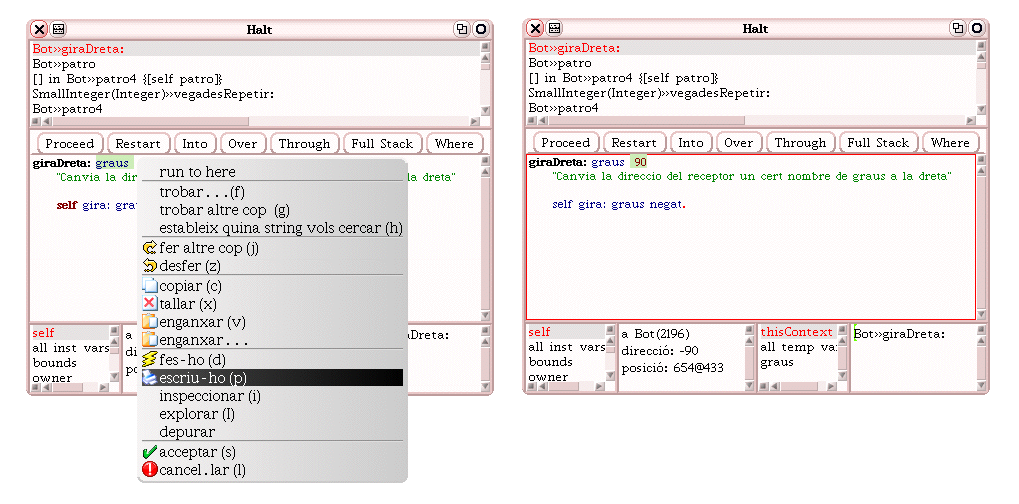
\includegraphics[scale=1.5]{Imatges/figura15-8.png}
\end{center}
\caption{\emph{Esquerra:} Seleccionant un argument i escrivint-lo.
\emph{Dreta:} El valor és escrit.}
\label{fig1508}
\end{figure}

\begin{figure}[h!]
\begin{center}
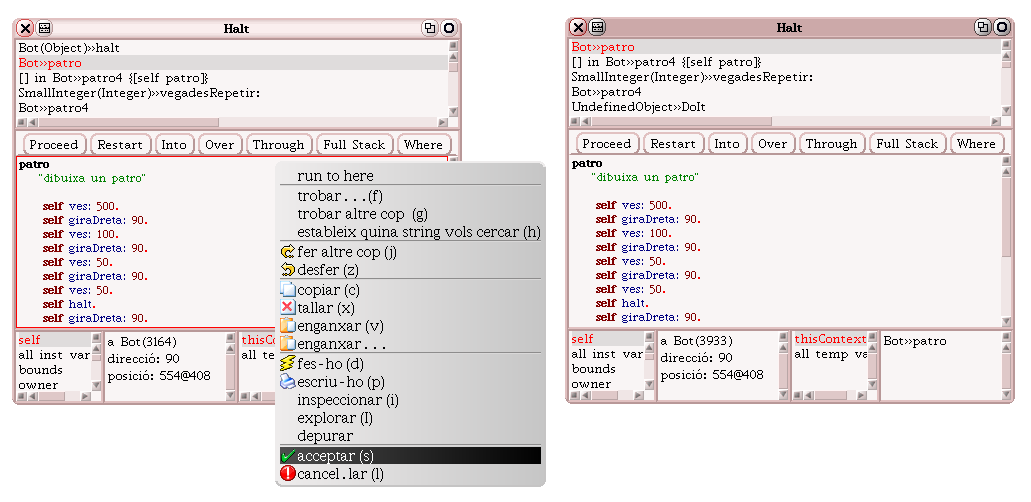
\includegraphics[scale=0.35]{Imatges/figura15-9.png}
\end{center}
\caption{\emph{Esquerra:} Editant la definició del mètode i recompilant-la.
\emph{Dreta:} El mètode \textsf{\upshape patro} ha estat recompilat.}
\label{fig1509}
\end{figure}

\newpage

Finalment, podeu \emph{modificar} la definició d'un mètode des del depurador editant el codi i acceptant-lo via l'opció del menú contextual
\textbf{acceptar} (veure figura~\ref{fig1509}). Per exemple, a la figura~\ref{fig1509}, hem tornat a començar el mètode prement el botó \textbf{Restart}; després hem editat el mètode en el mateix depurador, substituint el valor 100 del primer \textsf{ves:} pel valor 500. Aleshores hem recompilat el mètode amb l'opció \textbf{accept} del menú. Ara el robot es mourà 500 píxels si premem el botó \textbf{Proceed}.\index{metodes, definic@mètodes, definicions; modificar amb el depurador}

Això és una mica complicat, i en veure-ho per primera vegada ho podeu trobar una mica confús. Recordeu que el depurador us deixa executar totes les expressions d'un mètode pas a pas. Així doncs, si us plau, experimenteu amb el depurador i proveu tots els botons.
Estigueu tranquils, que cap robot prendrà mal en el procés.\index{metodes@mètodes!entrar sense executar|)}

\section{Corregir els errors}
\index{doesNotUnderstand mètode, efecte de}
\index{errors!corregir|(}
\index{metodes@mètodes!recompilar amb el depurador}
Us hem mostrat com obrir el depurador inserint l'expressió \textsf{self halt} en un mètode. També us hem ensenyat com podeu editar el codi d'un mètode en el depurador. Aquesta tècnica us permet utilitzar el depurador per corregir els vostres errors, és a dir, \emph{depurar} el vostre codi. Quan un objecte rep un missatge que no entén, Squeak us dóna l'oportunitat d'obrir el depurador. Quan un objecte no entén un missatge, Squeak envia a aquest objecte el missatge \textsf{doesNotUnderstand:} (això vol dir ``no entén'' literalment) juntament amb una representació del missatge. Per defecte, el mètode \textsf{doesNotUnderstand:} obre una capsa de diàleg per preguntar-vos si voleu obrir el depurador. Aleshores podeu utilitzar el depurador per explorar la pila dels mètodes executats i intentar entendre què ha anat malament.

\subsection{Exemple 1}

Per il·lustrar el procés, canvieu la primera línia del mètode \textsf{patro} a \textsf{self ves2: 100} i executeu l'expressió \textsf{Bot nou patro4}. Hauria d'aparèixer la capsa de diàleg del depurador (figura~\ref{fig1510}). La capsa de diàleg del depurador indica que el receptor, un robot creat per la classe \textsf{Bot}, no entén el missatge \textsf{ves2:}. Quan premeu el botó \textbf{Debug} a la capsa de diàleg, obriu el depurador, com podeu veure a l'esquerra de la figura~\ref{fig1510}. \index{patro, mètode!depurar}

El mètode al cim de la pila és el mètode \textsf{doesNotUnderstand:}, que és enviat al receptor d'un missatge quan el receptor no entén aquest missatge. El mètode directament davall és el mètode que conté el missatge que ha desencadenat l'error i per tant la crida al missatge \textsf{doesNotUnderstand:}. Aquí el mètode \textsf{patro} conté el missatge \textsf{ves2:}, que no és entès pel robot, com veieu a la figura~\ref{fig1510}.
\begin{figure}[h]
\begin{center}
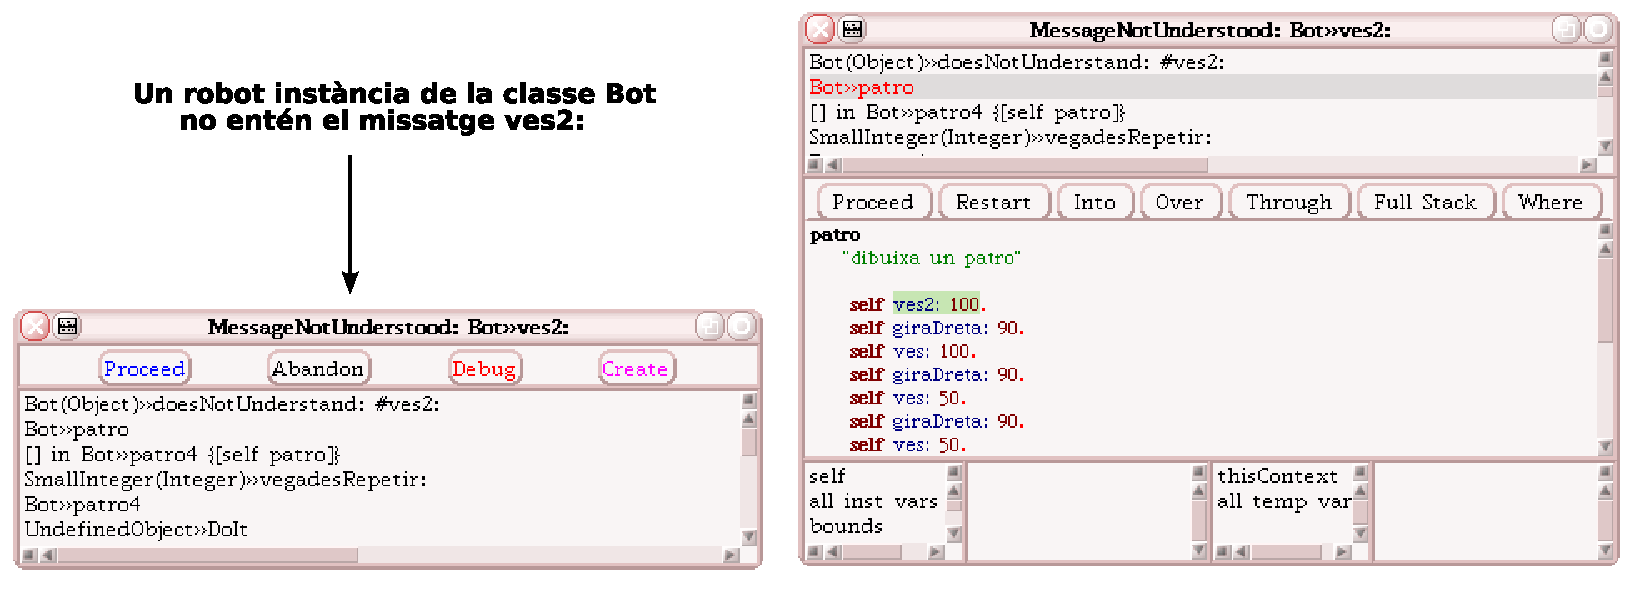
\includegraphics[scale=0.5]{Imatges/figura15-10.pdf}
\end{center}
\caption{\emph{Esquerra:} Un error \textsf{\upshape doesNotUnderstand:} ha succeït. 
\emph{Dreta:} Trobar el problema.}
\label{fig1510}
\end{figure}

\subsection{Exemple 2}
\index{nil valor, significat de|(}
Ara canvieu la primera línia del mètode \textsf{patro} a \textsf{self ves: nil} i executeu l'expressió \textsf{Bot nou patro4}. Hauríeu d'obtenir la capsa de diàleg del depurador mostrada a la figura~\ref{fig1511}. L'error és una mica difícil de trobar. Aquí, el títol de la capsa de diàleg \textsf{MessageNotUnderstood: UndefinedObject} indica que hi ha un missatge no entès enviat a \textsf{nil}, que és una instància de la classe \textsf{UndefinedObject}.
\begin{figure}[h!]
\begin{center}
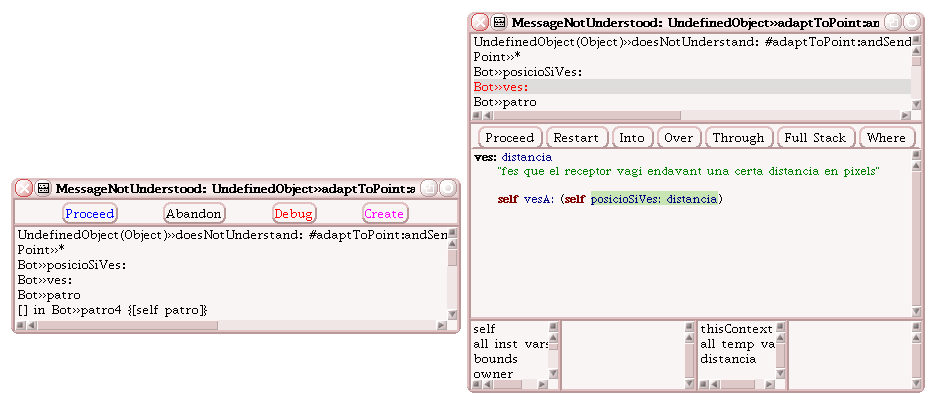
\includegraphics[scale=0.38]{Imatges/figura15-11.png}
\end{center}
\caption{\emph{Esquerra:} \textsf{\upshape nil} rep un missatge que no entén. 
\emph{Dreta:} Anar cap avall per la pila d'execució.}
\label{fig1511}
\end{figure}

El fet que \textsf{nil} sigui passat com a valor ha desencadenat un error després que s'executessin altres mètodes. Així doncs, heu d'anar avall a la pila, al punt on podeu entendre i corregir el vostre error. Per exemple, a la dreta de la figura~\ref{fig1511}, el segon mètode des de dalt deixa clar que alguna cosa no ha anat bé amb $*$, però el problema no ve d'aquest mètode. El mateix passa amb el següent mètode \textsf{ves:}. Si seleccioneu aquest mètode, podeu veure que el mètode \textsf{ves:} només passa l'argument que rep del mètode \textsf{patro} al mètode \textsf{posicioSiVes:}. Si seleccioneu el paràmetre \textsf{distancia} i escriviu el seu valor, obteniu \textsf{nil}. Això indica que l'error ve de més avall de la pila.

Finalment, podeu veure a l'esquerra de la figura~\ref{fig1512} que \textsf{nil} es passa com a argument, i no un nombre, que és el que espera el mètode \textsf{ves:}. Ara podeu corregir l'error editant el mètode \textsf{patro} i canviar \textsf{self ves: nil} per \textsf{self ves: 100}, acceptant els canvis mitjançant el menú i prement el botó \textbf{Proceed} per continuar l'execució.\index{Proceed, botó; utilitzar al depurador}\index{patro, mètode!recompilar amb el depurador}

Aquest exemple utilitzant \textsf{nil} com a argument d'un missatge \textsf{ves:} provoca un error fàcil d'identificar. És possible que cometeu ocasionalment errors trivials com aquest, però el que generalment haureu d'afrontar és una gran varietat de situacions inesperades que provoquen errors. Tot i així, el procés és el mateix: Heu d'utilitzar el depurador per explorar la pila d'execució, i comprovar els valors dels arguments fins que pugueu entendre què és el que ha anat malament. Us podeu trobar amb la situació que també calgui modificar el codi, no només els arguments dels missatges. \index{errors!corregir|)} \index{metodes, definic@mètodes, definicions; modificar amb el depurador} \index{nil valor, significat de|)}
\begin{figure}[hb]
\begin{center}
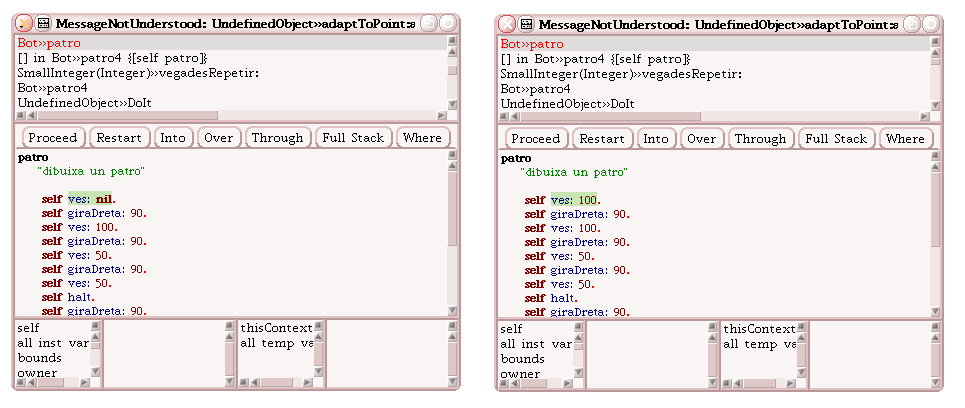
\includegraphics[scale=0.4]{Imatges/figura15-12.png}
\end{center}
\caption{\emph{Esquerra:} Editar i recompilar la definició del mètode. 
\emph{Dreta:} El mètode \textsf{\upshape patro} ha estat recompilat.}
\label{fig1512}
\end{figure}

\section{Resum}

\begin{itemize}
\item A Smalltalk, el valor d'una variable no inicialitzada és per defecte l'objecte \textsf{nil}, que s'utilitza per representar un valor indefinit.
\item El depurador d'Squeak és una eina que us permet explorar els mètodes ja executats. Utilizant el depurador, podeu escriure els valors dels arguments, modificar la definició dels mètodes, i continuar l'execució.
\item Per obrir el depurador explícitament, inseriu l'expressió \textsf{self halt} en un mètode. Quan l'expressió \textsf{self halt} s'executa, podeu obrir el depurador.
\end{itemize}

\chapter{Descompondre per recompondre} 
\label{cap16}

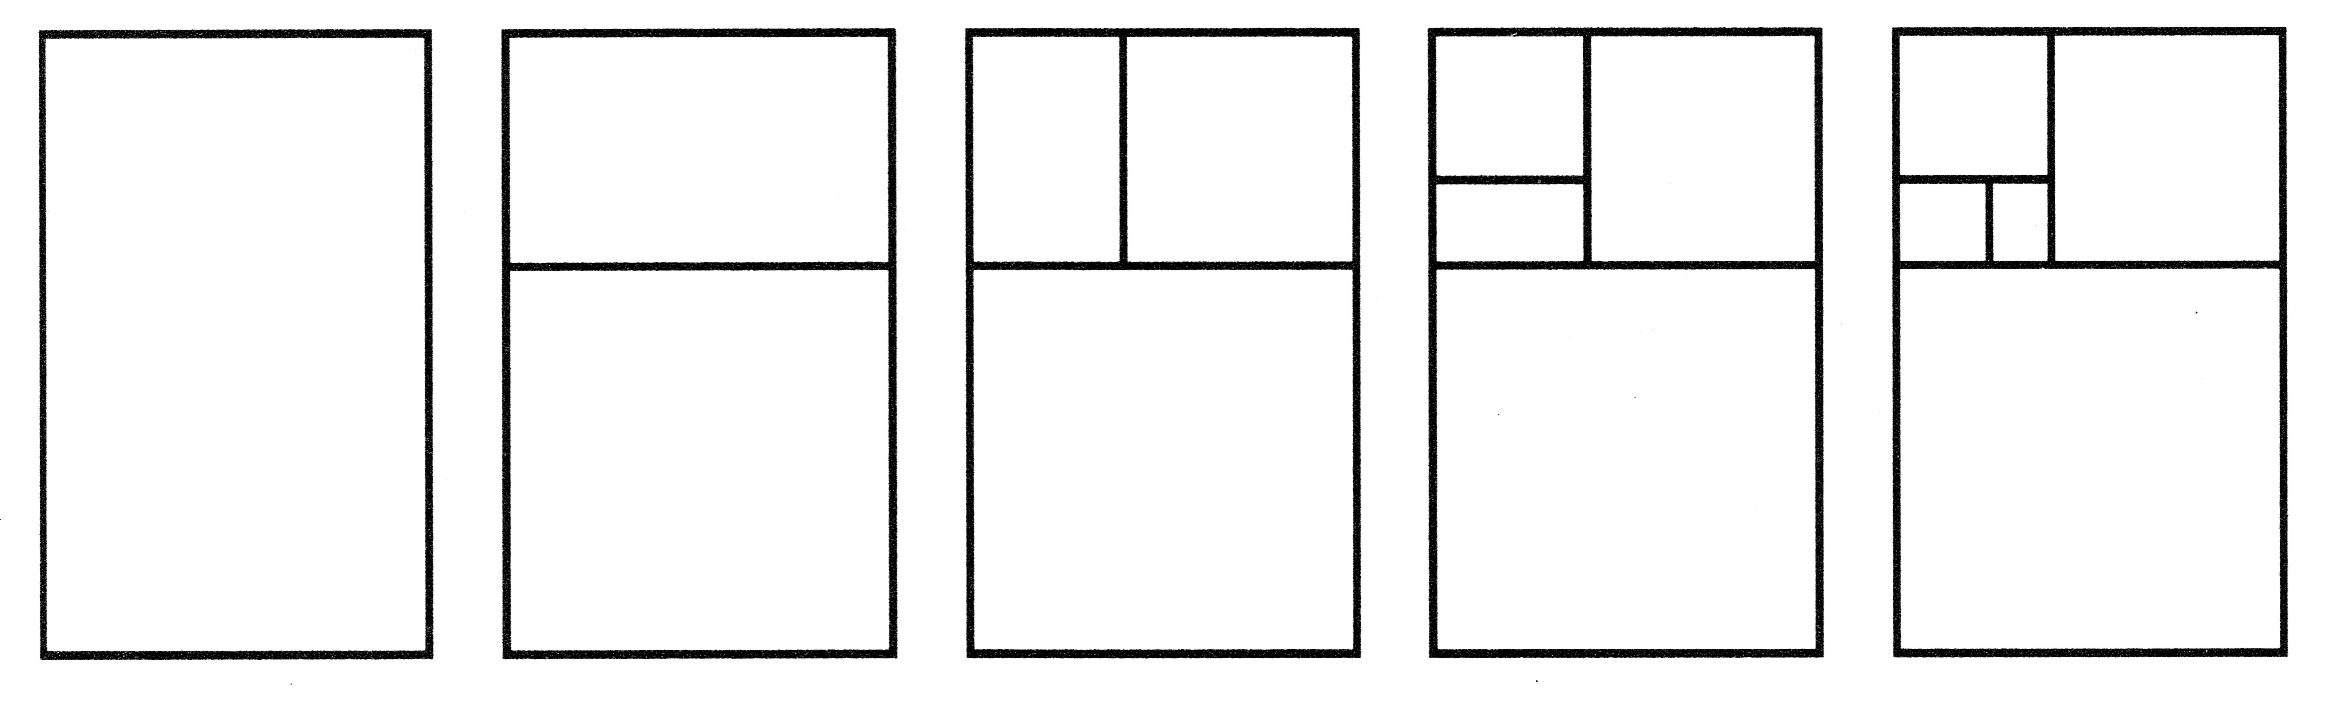
\includegraphics[scale=0.15]{Imatges/figura16-0.jpg}
\vspace*{2mm}

En aquest capítol voldríem ensenyar-vos que una bona aproximació per resoldre un problema és \emph{descompondre} el problema en petits problemes més senzills de resoldre, i després \emph{compondre} les solucions dels problemes més petits per resoldre el problema original. Sovint, definir i utilitzar un cert nombre de mètodes simples us permet resoldre un problema complex d'una manera molt més senzilla i natural que intentar resoldre el problema tot de cop. Aquest és un altre exemple del poder de l'abstracció que vam introduir al capítol~\ref{cap12}.\index{compondre solucions, significat de} \index{descompondre problemes, significat de}

Desafortunadament, tot i que la decomposició de problemes en problemes més petits és una tècnica molt valuosa, no hi ha cap manera sistemàtica de descompondre un problema. Només amb experiència i molta prova i error és possible aprendre i desenvolupar alguna intuïció sobre la resolució de problemes. En aquest capítol, us proposo alguns problemes, petits però no trivials, que hauríeu de provar de resoldre. Intenteu descompondre'ls en problemes més petits i amb les solucions d'aquests compondre una solució al problema plantejat en un principi. Els problemes plantejats en aquest capítol són els exercicis més complexos de tot el llibre, així que no us desanimeu si no els resoleu a la primera. Tot i així, és molt important que ho intenteu.

\section{Laberints i espirals}
\index{laberints, crear|(}
Al capítol~\ref{cap10}, vau fer experiments amb repeticions i variables. En aquell moment, no sabíeu que podíeu utilitzar mètodes escrits per vosaltres mateixos. Ara us suggerim que torneu a fer aquells experiments utilitzant mètodes com \textsf{quadrat:} i que definiu mètodes amb múltiples arguments per ajudar-vos. Com ja vam mencionar, resoldre problemes complexos utilitzant mètodes més senzills és una tasca difícil que només es pot aprendre amb la pràctica. Per tant, us encoratgem a fer tots els experiments d'aquest capítol, i, de fet, hauríeu de provar de trobar més d'una solució per a cada un d'ells. Intenteu veure com la solució a un problema pot ser expressada a un cert nivell elevat d'abstracció. Aquesta aproximació fa que el problema global sigui més senzill d'expressar. Per exemple, per dibuixar una piràmide de quadrats, podríeu simplement dibuixar un gran nombre de quadrats. Però a un nivell més alt d'abstracció podríeu veure la piràmide com un cert nombre de fileres de diferent mida amb quadrats com a components, i provar de definir i utilitzar un mètode que dibuixi fileres de \emph{n} quadrats.

\subsection{Quadrats centrats}
\index{quadrats centrats, crear|(}
Els experiments següents us proporcionen més oportunitats de practicar les vostres habilitats. Imagineu diferents estratègies per resoldre aquests problemes. Una pista: definiu un mètode \textsf{quadratCentrat: mida} que dibuixi un quadrat centrat al voltant del robot, i que després de dibuixar el quadrat faci que el robot es desplaci a la seva posició original.

\begin{center}
\colorbox{black}{\makebox[\textwidth]{  \color{white} {\large {\bfseries Experiment 16-1 (ones quadrades en un estany quadrat)}}}}
\end{center}
\index{ones quadrades en un estany quadrat, Experiment}
\index{Experiments!ones quadrades en un estany quadrat}
{\small
\noindent
Mitjançant la composició de mètodes, dibuixeu la figura que veieu més avall.}
\begin{center}

\includegraphics[scale=0.25]{Imatges/figuraE16-1.png} 
\end{center}
\noindent
\rule{\textwidth}{3pt}
\newpage
\begin{center}
\colorbox{black}{\makebox[\textwidth]{  \color{white} {\large {\bfseries Experiment 16-2 (un passadís)}}}}
\end{center}
\index{passadis @un passadís, Experiment}
\index{Experiments!passadis @un passadís}
{\small
\noindent
Mitjançant la composició de mètodes, dibuixeu la figura que veieu més avall.}
\begin{center}
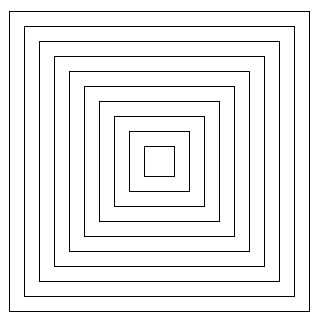
\includegraphics[scale=0.4]{Imatges/figuraE16-2.png} 
\end{center}
\noindent
\rule{\textwidth}{3pt}

\vspace*{5mm}

\begin{center}
\colorbox{black}{\makebox[\textwidth]{  \color{white} {\large {\bfseries Experiment 16-3 (quadrats russos)}}}}
\end{center}
\index{Quadrats Russos, Experiment}
\index{Experiments!Quadrats Russos}
{\small
\noindent
Utilitzant el mètode \textsf{quadrat:} per construir quadrats de diferents mides, com podeu veure a la figura.}
\begin{center}
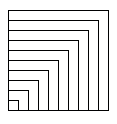
\includegraphics[scale=1]{Imatges/figuraE16-3.png} 
\end{center}
\noindent
\rule{\textwidth}{3pt}
\index{quadrats centrats, crear|)} \index{laberints, crear|)}
\newpage
\subsection{Espirals}
\index{espirals, crear}
\index{parametres@paràmetres!utillitzar amb espirals}
Les espirals d'aquest capítol s'han dibuixat totes utilitzant només segments rectes, angles i repeticions. No tenen cap corba; el robot dibuixa una línia recta a mida que va endavant, gira un cert angle i repeteix el procés.

Al primer grup d'espirals, la longitud de cada segment canvia una mica respecte de la del segment previ. El robot gira el mateix angle després de cada segment recte. Aquestes espirals s'anomenen \emph{espirals d'angle constant} ja que l'angle no canvia.

\begin{center}
\colorbox{black}{\makebox[\textwidth]{  \color{white} {\large {\bfseries Experiment 16-4 (una espiral d'angle constant)}}}}
\end{center}
\index{espiral d'angle constant@una espiral d'angle constant, Experiment}
\index{Experiments!espiral d'angle constant@una espiral d'angle constant}
\index{espiral d'angle constant, definició}
{\small
\noindent
Definiu un mètode \textsf{espiralAngleConstant:} que dibuixi una espiral d'angle constant. L'angle que el robot ha de girar és l'únic paràmetre. Canvieu la distància que el robot viatja en la mateixa quantitat per a cada segment. Divertiu-vos i proveu diferents angles; podeu crear dibuixos molt bonics. L'\emph{script} següent ha creat l'espiral que veieu aquí.}\\
\begin{center}
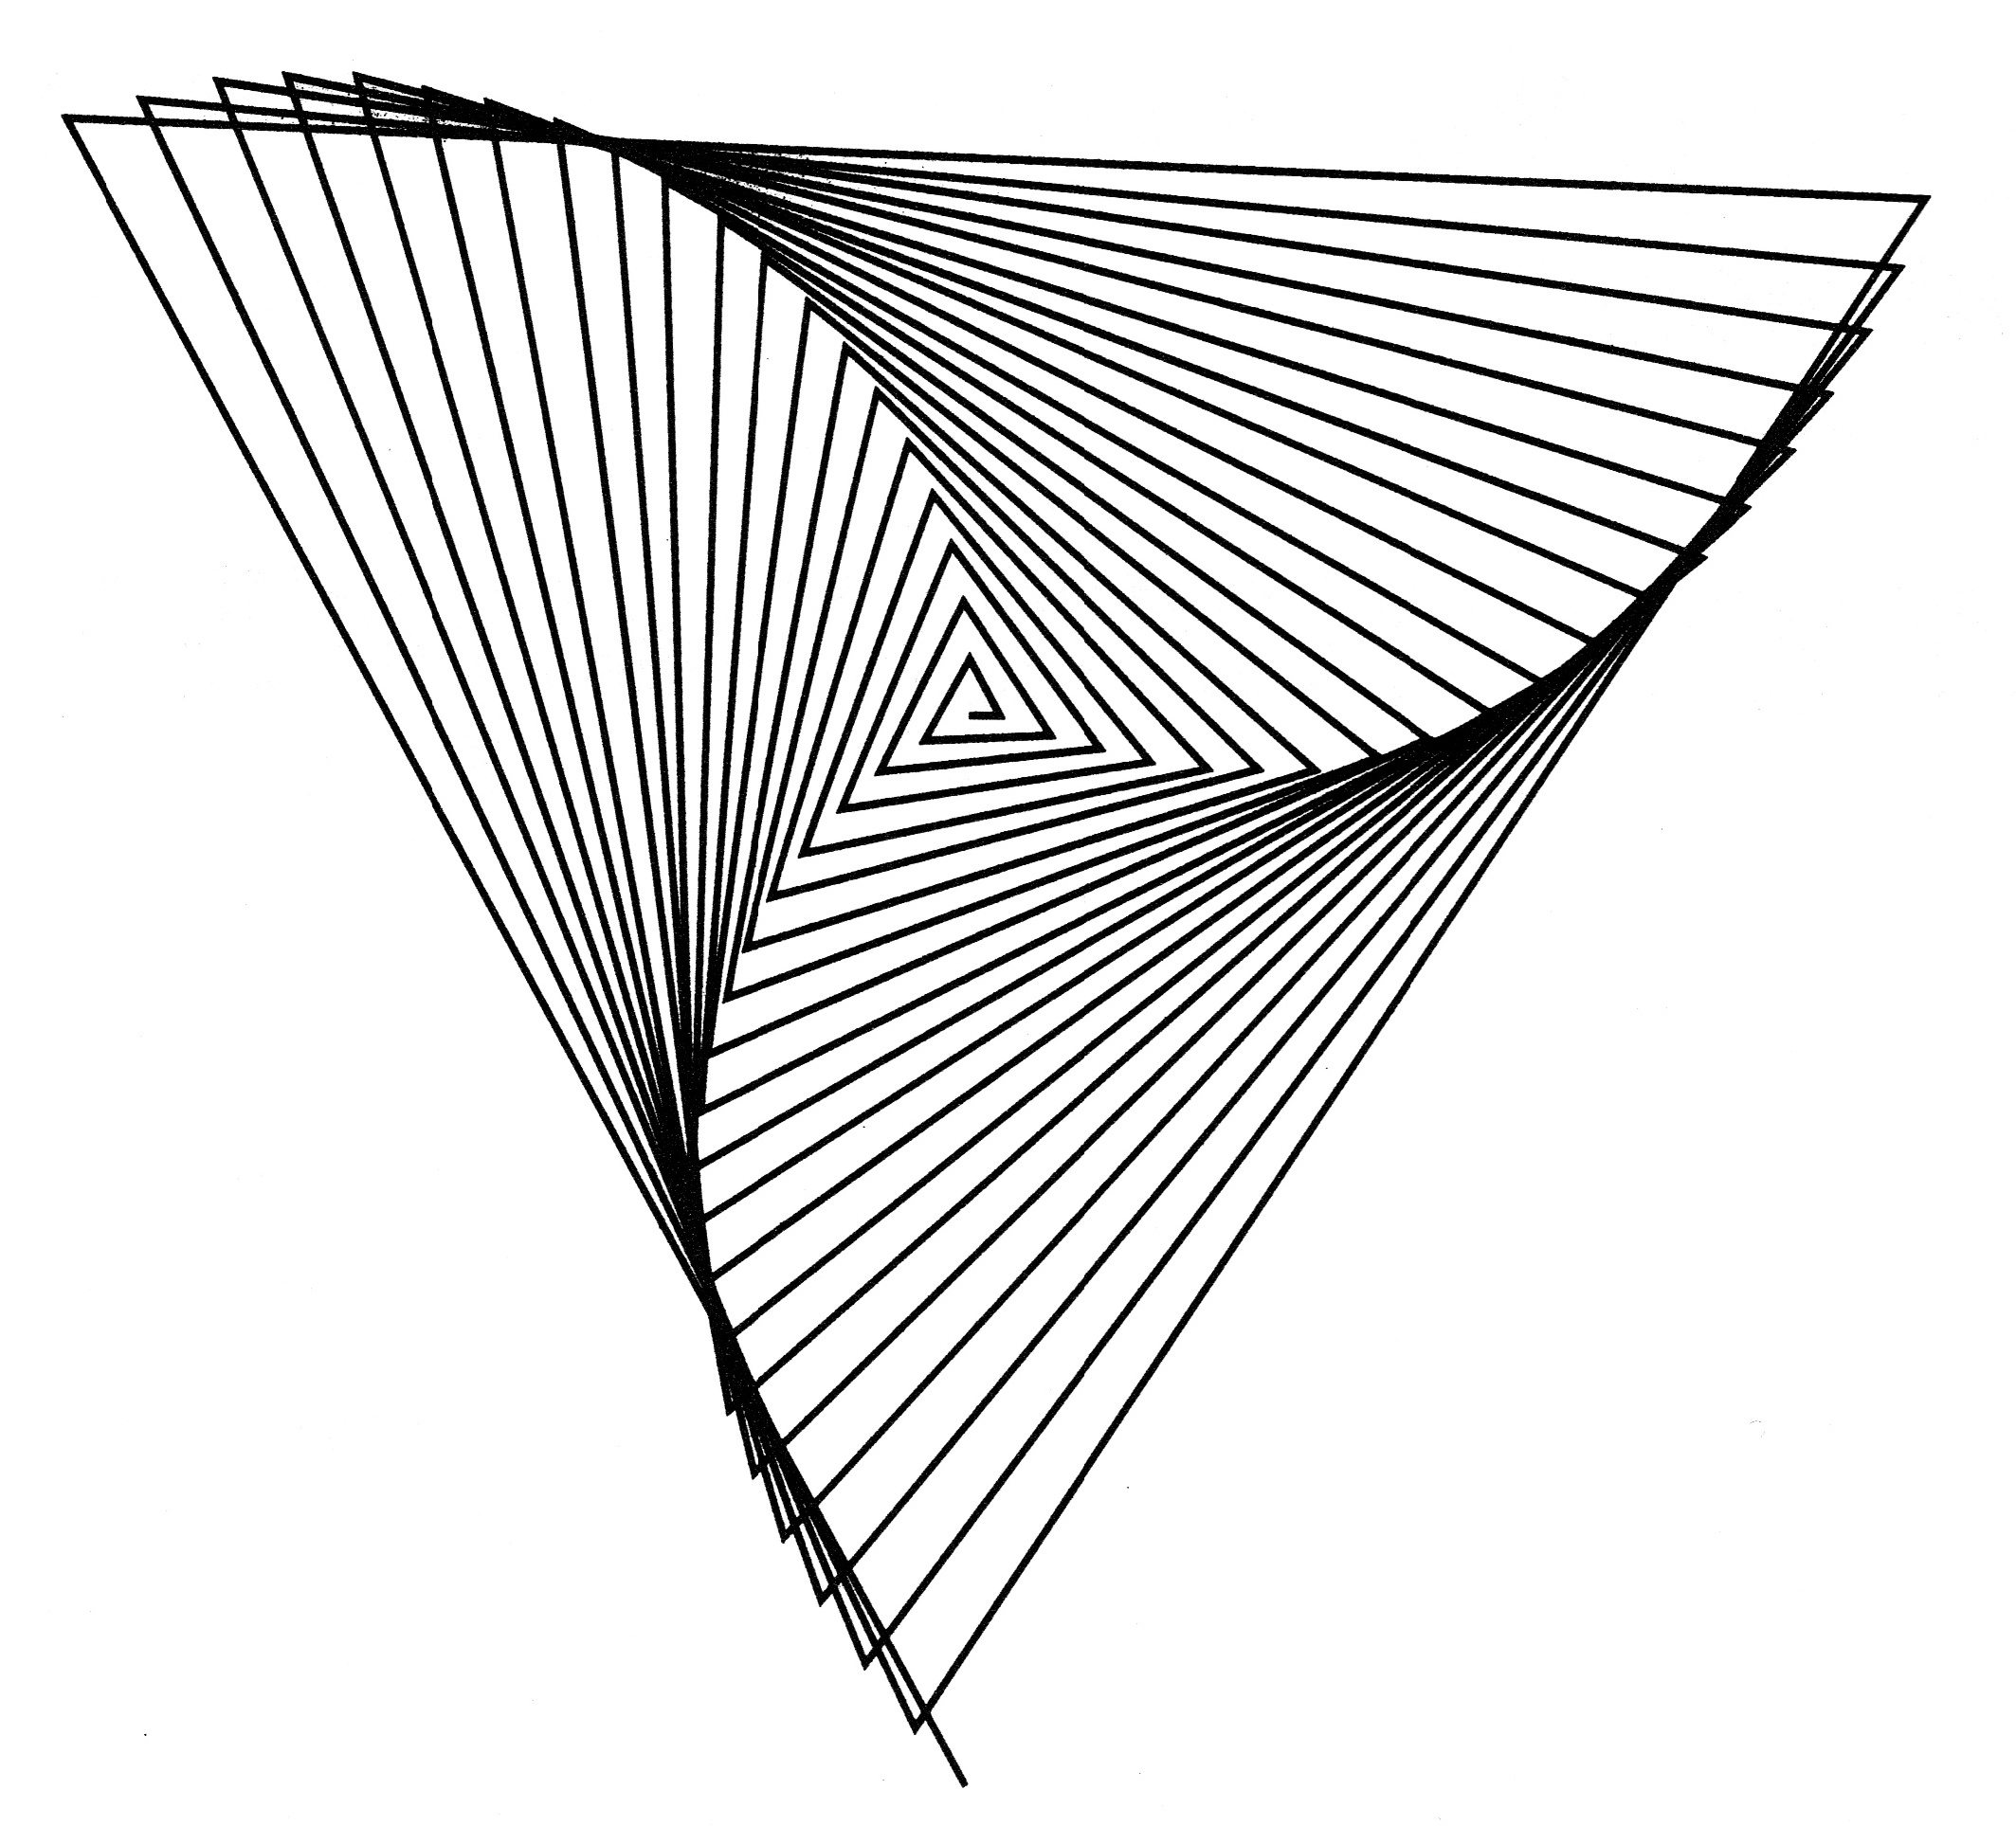
\includegraphics[scale=0.06]{Imatges/figuraE16-4.jpg} 
\end{center}
\noindent
{\small
\textsf{
\begin{tabbing}
\hspace{5mm} \= \kill
$|$ pica $|$\\
pica := Bot nou.\\
pica espiralAngleConstant: 121
\end{tabbing}
}}
\noindent
\rule{\textwidth}{3pt}

\begin{center}
\colorbox{black}{\makebox[\textwidth]{  \color{white} {\large {\bfseries Experiment 16-5 (una altra espiral)}}}}
\end{center}
\index{altra espiral@una altra espiral, Experiment}
\index{Experiments!altra espiral@una altra espiral}
{\small
\noindent
En l'experiment anterior, a cada pas afegíeu el mateix nombre a la distància a què el robot es desplaçava. Ara experimenteu calculant la mida d'un costat, no afegint una constant a la longitud del costat previ, sinó multiplicant-la per una proporció constant. Pareu atenció! Multiplicar per 1.1 implica un increment d'un 10 per cent.}\\
\noindent
\rule{\textwidth}{3pt}

\begin{center}
\colorbox{black}{\makebox[\textwidth]{  \color{white} {\large {\bfseries Experiment 16-6 (una espiral amb quatre paràmetres)}}}}
\end{center}
\index{espiral amb quatre@una espiral amb quatre paràmetres, Experiment}
\index{Experiments!espiral amb quatre@una espiral amb quatre paràmetres}
{\small
\noindent
El mètode \textsf{espiralAngleConstant:} depèn de quatre valors. Aquests són el \emph{nombre de segments}, la \emph{longitud inicial} del primer segment, la \emph{quantitat afegida a cada segment}, i l'\emph{angle} que gira el robot. Definiu un mètode \textsf{espiralSegments:longitudInicial:incrementLongitud:angleConstant:} que dibuixi qualsevol espiral canviant aquests quatre paràmetres. Proveu, per exemple, l'\emph{script} següent, que dibuixa dues espirals diferents.}
\noindent
{\small
\textsf{
\begin{tabbing}
\hspace{5mm} \= \kill
$|$ pica $|$\\
pica := Bot nou.\\
pica espiralSegments: 50 longitudInicial: 10 incrementLongitud: 3 angleConstant: 144.\\
pica color: Color vermell.\\
pica espiralSegments: 120 longitudInicial: 1 incrementLongitud: 3 angleConstant: 12.
\end{tabbing}}}
\noindent
\rule{\textwidth}{3pt}
\begin{figure}[h!]
\begin{center}
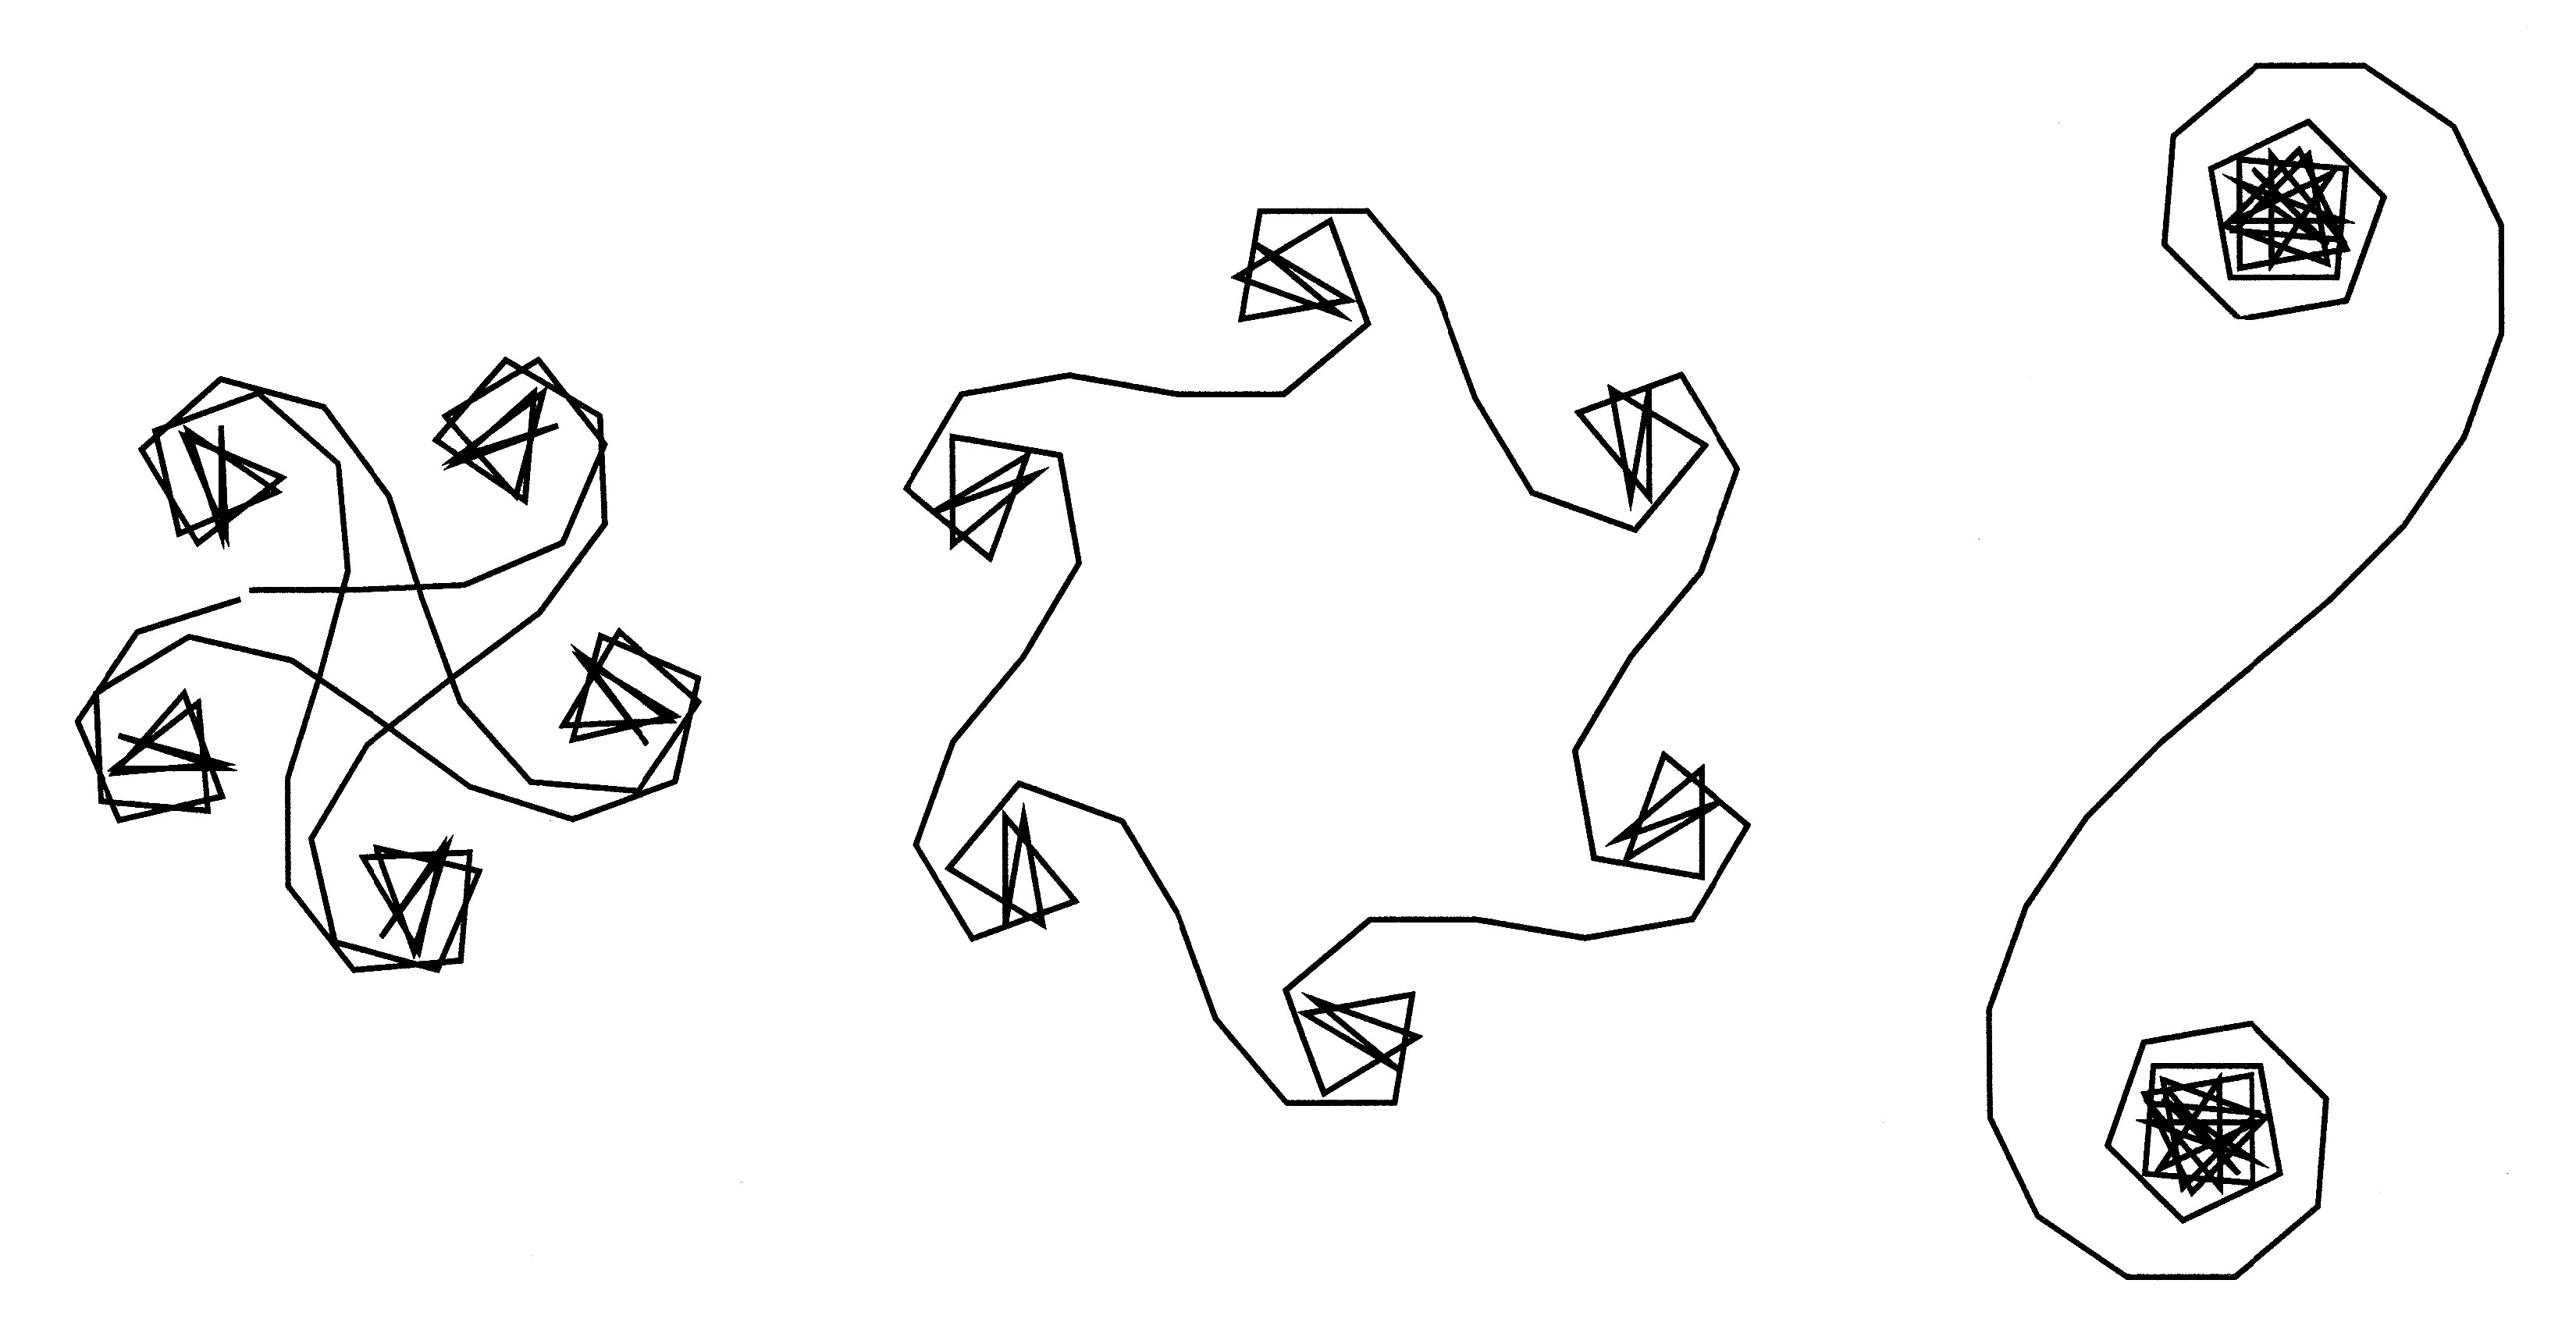
\includegraphics[scale=0.07]{Imatges/figura16-1.jpg}
\end{center}
\caption{\emph{Esquerra:} Iteracions: 90, angle inicial: 2, increment: 20, longitud: 30.
\emph{Mig:} Iteracions: 72, angle inicial: 40, increment: 30, longitud: 30. 
\emph{Dreta:} Iteracions: 100, angle inicial: 40, increment: 5, longitud: 23.}
\label{fig1601}
\end{figure}
\begin{center}
\colorbox{black}{\makebox[\textwidth]{  \color{white} {\large {\bfseries Experiment 16-7 (espirals amb distància constant)}}}}
\end{center}
\index{espirals amb distància constant, Experiment}
\index{Experiments!espirals amb distància constant}
{\small
\noindent
Fins ara heu creat espirals \emph{canviant la distància} que el robot es movia endavant, i el robot sempre girava \emph{el mateix angle}. Ara experimenteu fent el contrari: manteniu la distància constant, i incrementeu l'angle una quantitat fixada després de cada segment. Per a aquests experiments, definiu un mètode amb quatre arguments: el nombre de repeticions, el valor inicial de l'angle, l'increment de l'angle, i la longitud d'un segment. Com podeu veure a la figura~\ref{fig1601}, que mostra tres espirals, fer prediccions de les corbes que aquest mètode pot generar és més aviat difícil. Jugueu amb diferents valors. Divertiu-vos!}\\
\noindent
\rule{\textwidth}{3pt}

\newpage

\begin{center}
\colorbox{black}{\makebox[\textwidth]{  \color{white} {\large {\bfseries Experiment 16-8 (espirals a partir de quadrats)}}}}
\end{center}
\index{espirals a partir de quadrats, Experiment}
\index{Experiments!espirals a partir de quadrats}
{\small
\noindent
Si canvieu el mètode que heu definit a l'Experiment 16-7 per a que dibuixi un petit quadrat en lloc d'una línia, podeu aconseguir figures molt extravagants, com la que veieu a la figura~\ref{fig1602}.}\\
\noindent
\rule{\textwidth}{3pt}

\begin{figure}[h]
\begin{center}
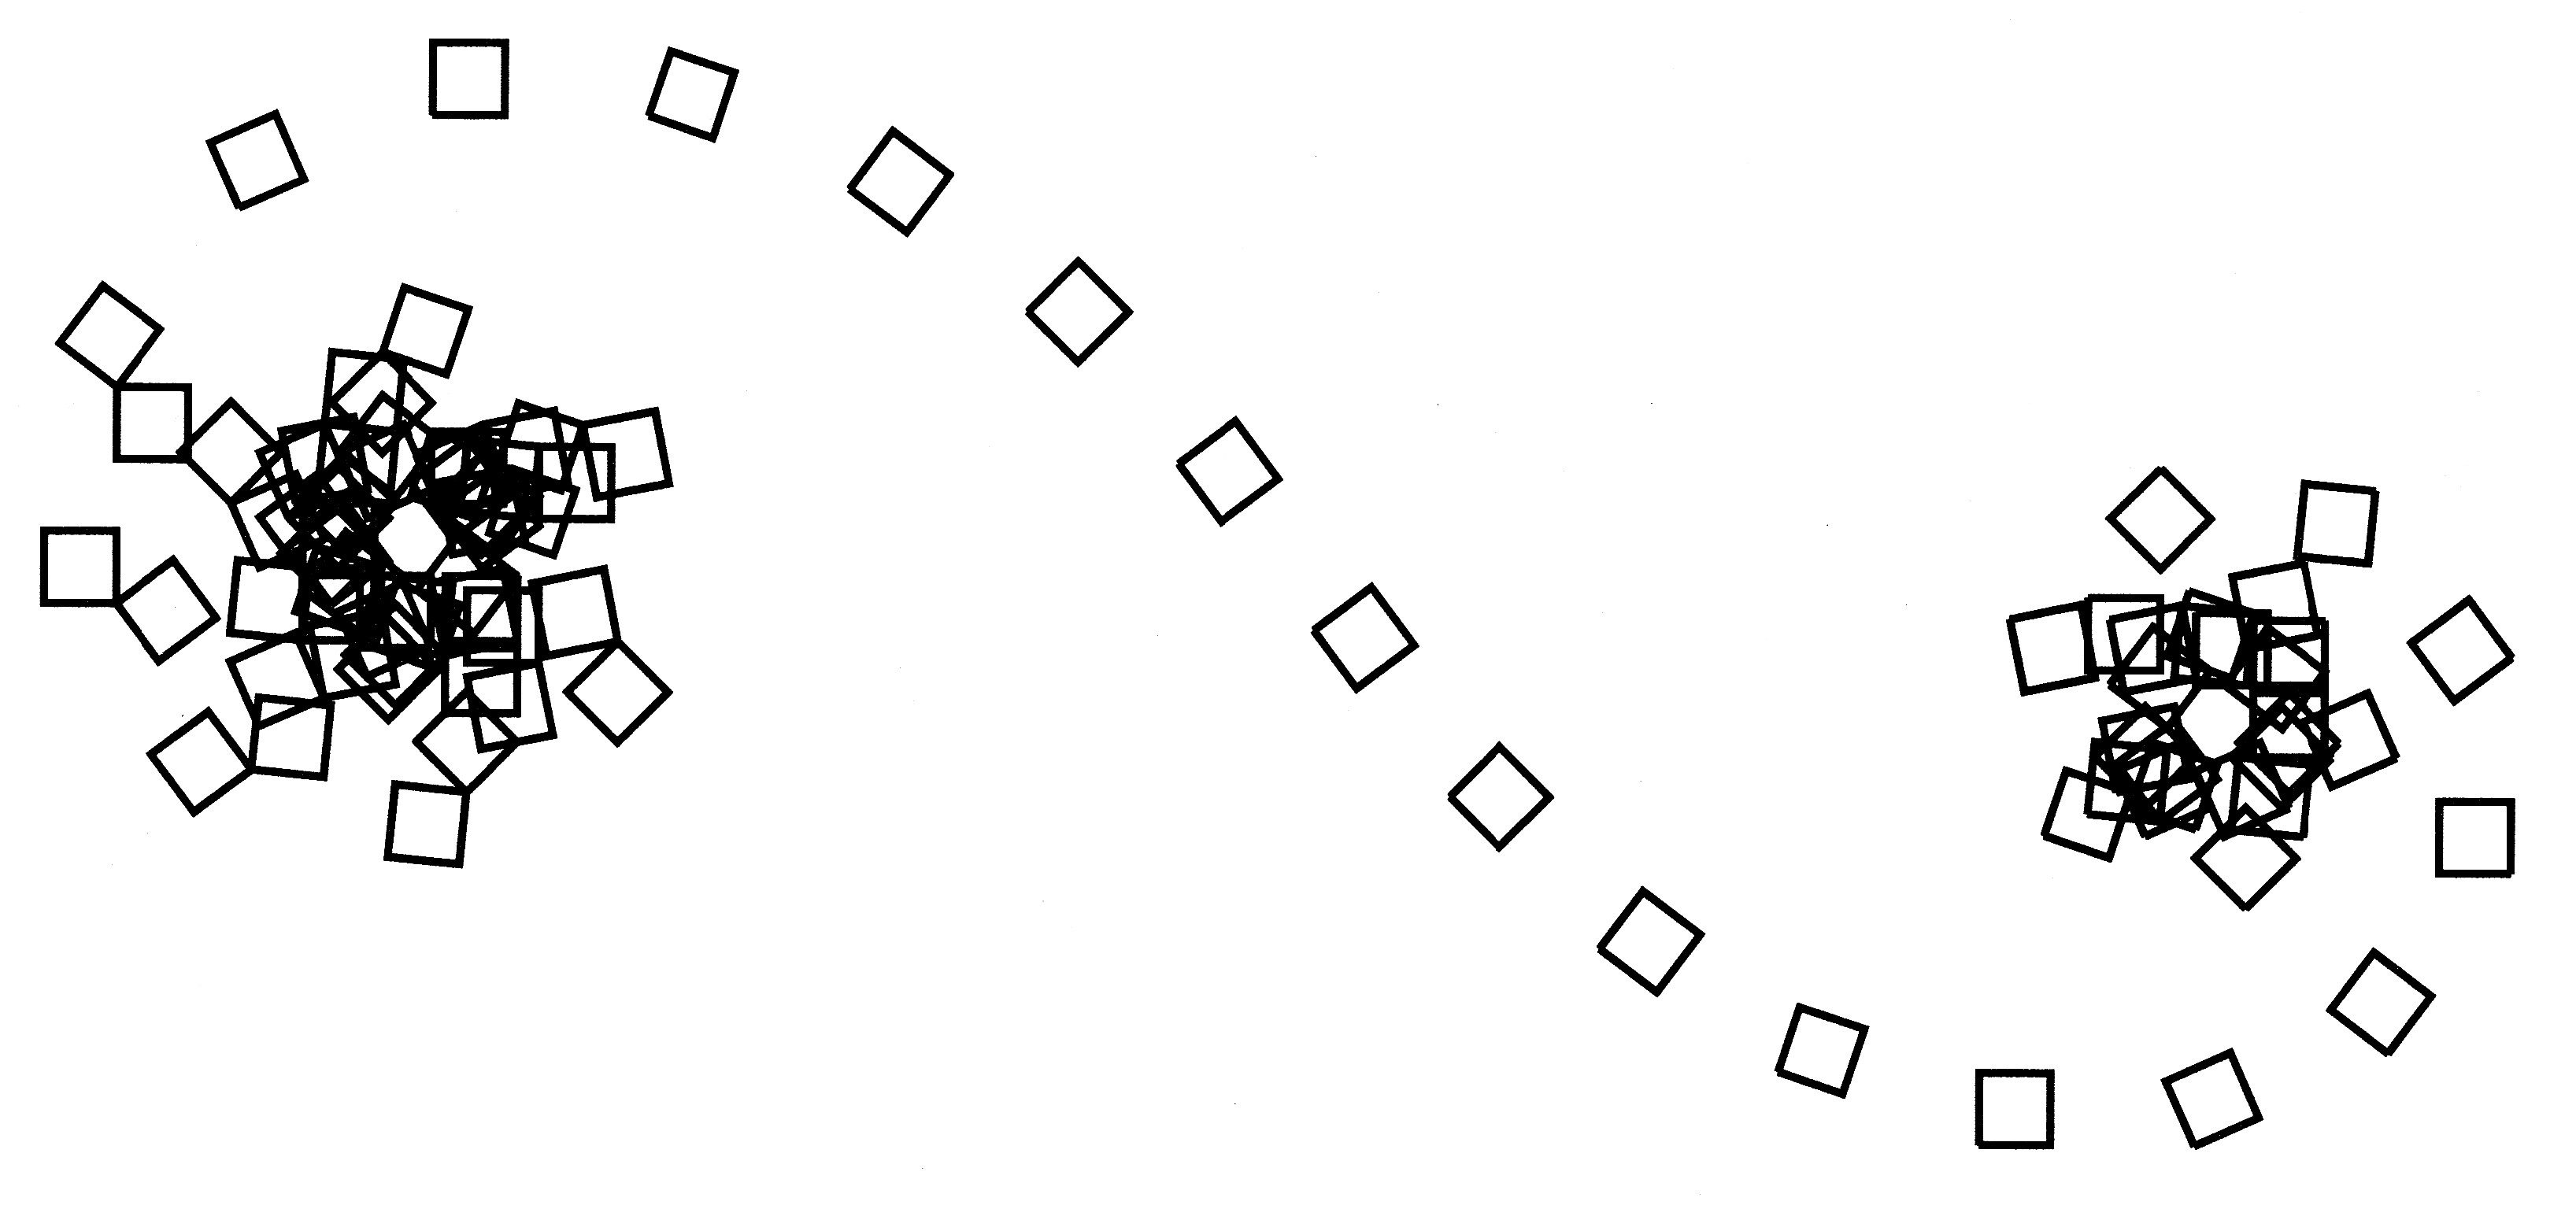
\includegraphics[scale=0.1]{Imatges/figura16-2.jpg}
\end{center}
\caption{Dibuix d'una ``espiral'' de longitud constant utilitzant quadrats.}
\label{fig1602}
\end{figure}

\begin{center}
\colorbox{black}{\makebox[\textwidth]{  \color{white} {\large {\bfseries Experiment 16-9 (una espiral a partir de línies)}}}}
\end{center}
\index{espiral a partir de línies@una espiral a partir de línies, Experiment}
\index{Experiments!espiral a partir de línies@una espiral a partir de línies}
\index{linies@línies!crear espirals a partir de}
{\small
\noindent
Intenteu reproduir la figura de més avall. Algunes indicacions: comenceu amb una longitud de 5 i incrementeu-la de 3 en 3, i feu que el robot giri un angle de 178 graus.}
\begin{center}
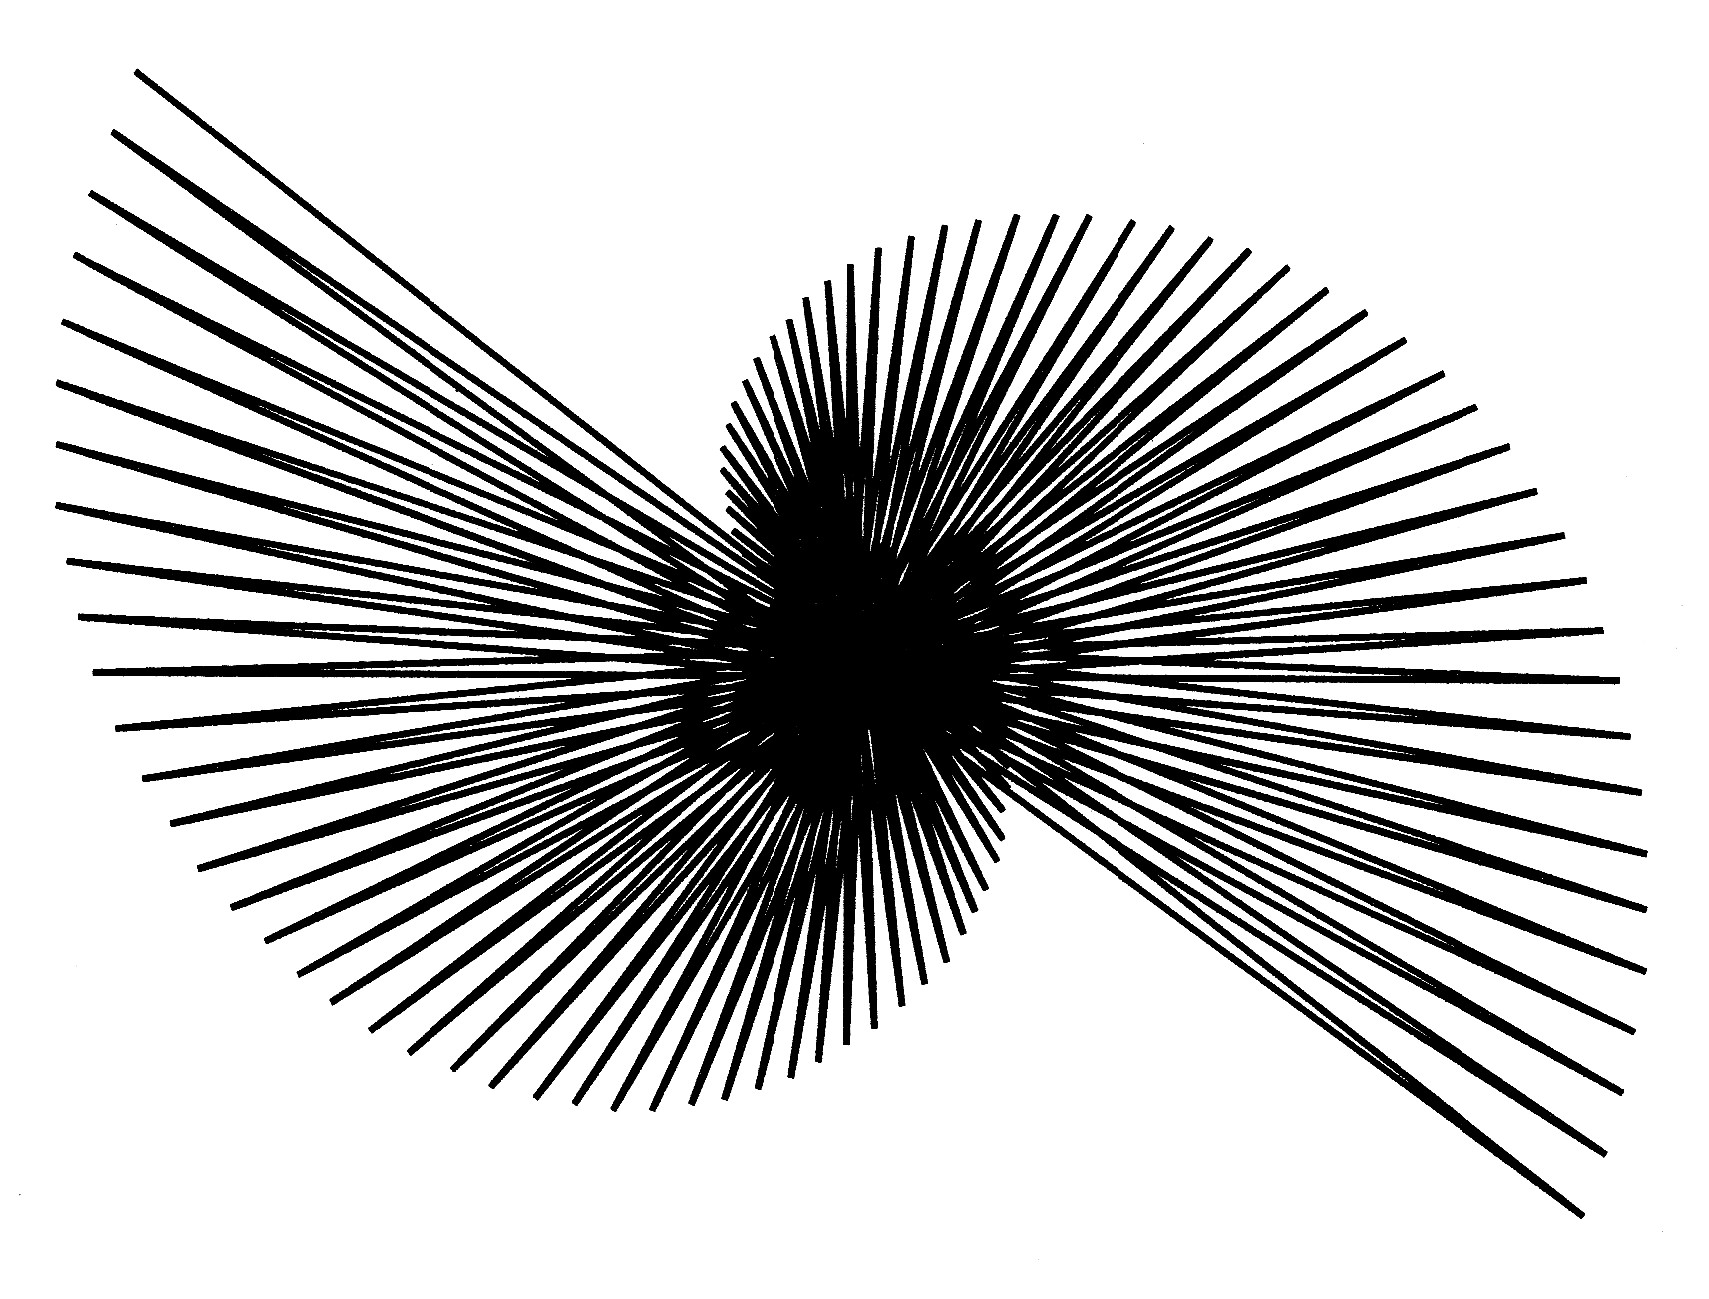
\includegraphics[scale=0.075]{Imatges/figuraE16-9.jpg} 
\end{center}
\noindent
\rule{\textwidth}{3pt}

\section{Rectangles d'or}
\index{rectangles d'or|seealso{rectangles}}
\index{rectangles d'or!dibuixar|(}
\index{rectangles d'or!imbricar}
\index{secció àuria, calcular}
\index{metodes@mètodes!definir per dibuixar rectangles d'or|(}
Ara és el moment d'escriure alguns mètodes per dibuixar el famós rectangle d'or que vam introduir al capítol~\ref{cap8}. Us encoratgem a provar els vostres propis mètodes abans de llegir cap solució. Per a alguns dels experiments no donem cap solució. En lloc d'això, us oferim algunes pistes.

Un rectangle d'or és un rectangle amb la propietat que si traieu un quadrat d'un extrem del rectangle, amb costat de longitud igual a l'amplada del rectangle, allò que queda és també un rectangle d'or. Per exemple, el rectangle 2 de la figura~\ref{fig1603} està compost d'un quadrat a la part de sota i un altre rectangle d'or a la part de dalt. Al rectangle 3, el rectangle d'or dins el rectangle 2 ha estat dividit en un quadrat i un rectangle d'or més petit encara. El procés es repeteix en els rectangles 4 i 5.

No és difícil demostrar que per tal que un rectangle tingui aquesta propietat, la proporció entre llargada i amplada ha de ser $\frac{1 + \sqrt{5}}{2}$ (que és aproximadament igual a $1.6$)\footnote{Si l'amplada d'un rectangle d'or és $1$ i la seva llargada és $x$, quan traieu un quadrat del rectangle d'or, el rectangle d'or més petit que queda té llargada $1$ i amplada $x-1$. Com que aquests rectangles són similars, la proporció entre els seus costats ha de ser la mateixa. Traient els denominadors i resolent l'eqüació quadràtica resultant posem de manifest que la llargada $x$ del rectangle original ha de ser igual a la raó àuria.}. Aquest nombre especial s'anomena la \emph{raó àuria} o la \emph{secció àuria}. Podem calcular-lo a Smalltalk amb l'expressió \textsf{1 + 5 sqrt / 2}.

El problema que us estem plantejant és dibuixar diversos rectangles d'or, cada un dins de l'anterior, com podeu veure a la figura~\ref{fig1603}.
\begin{figure}[h!]
\begin{center}
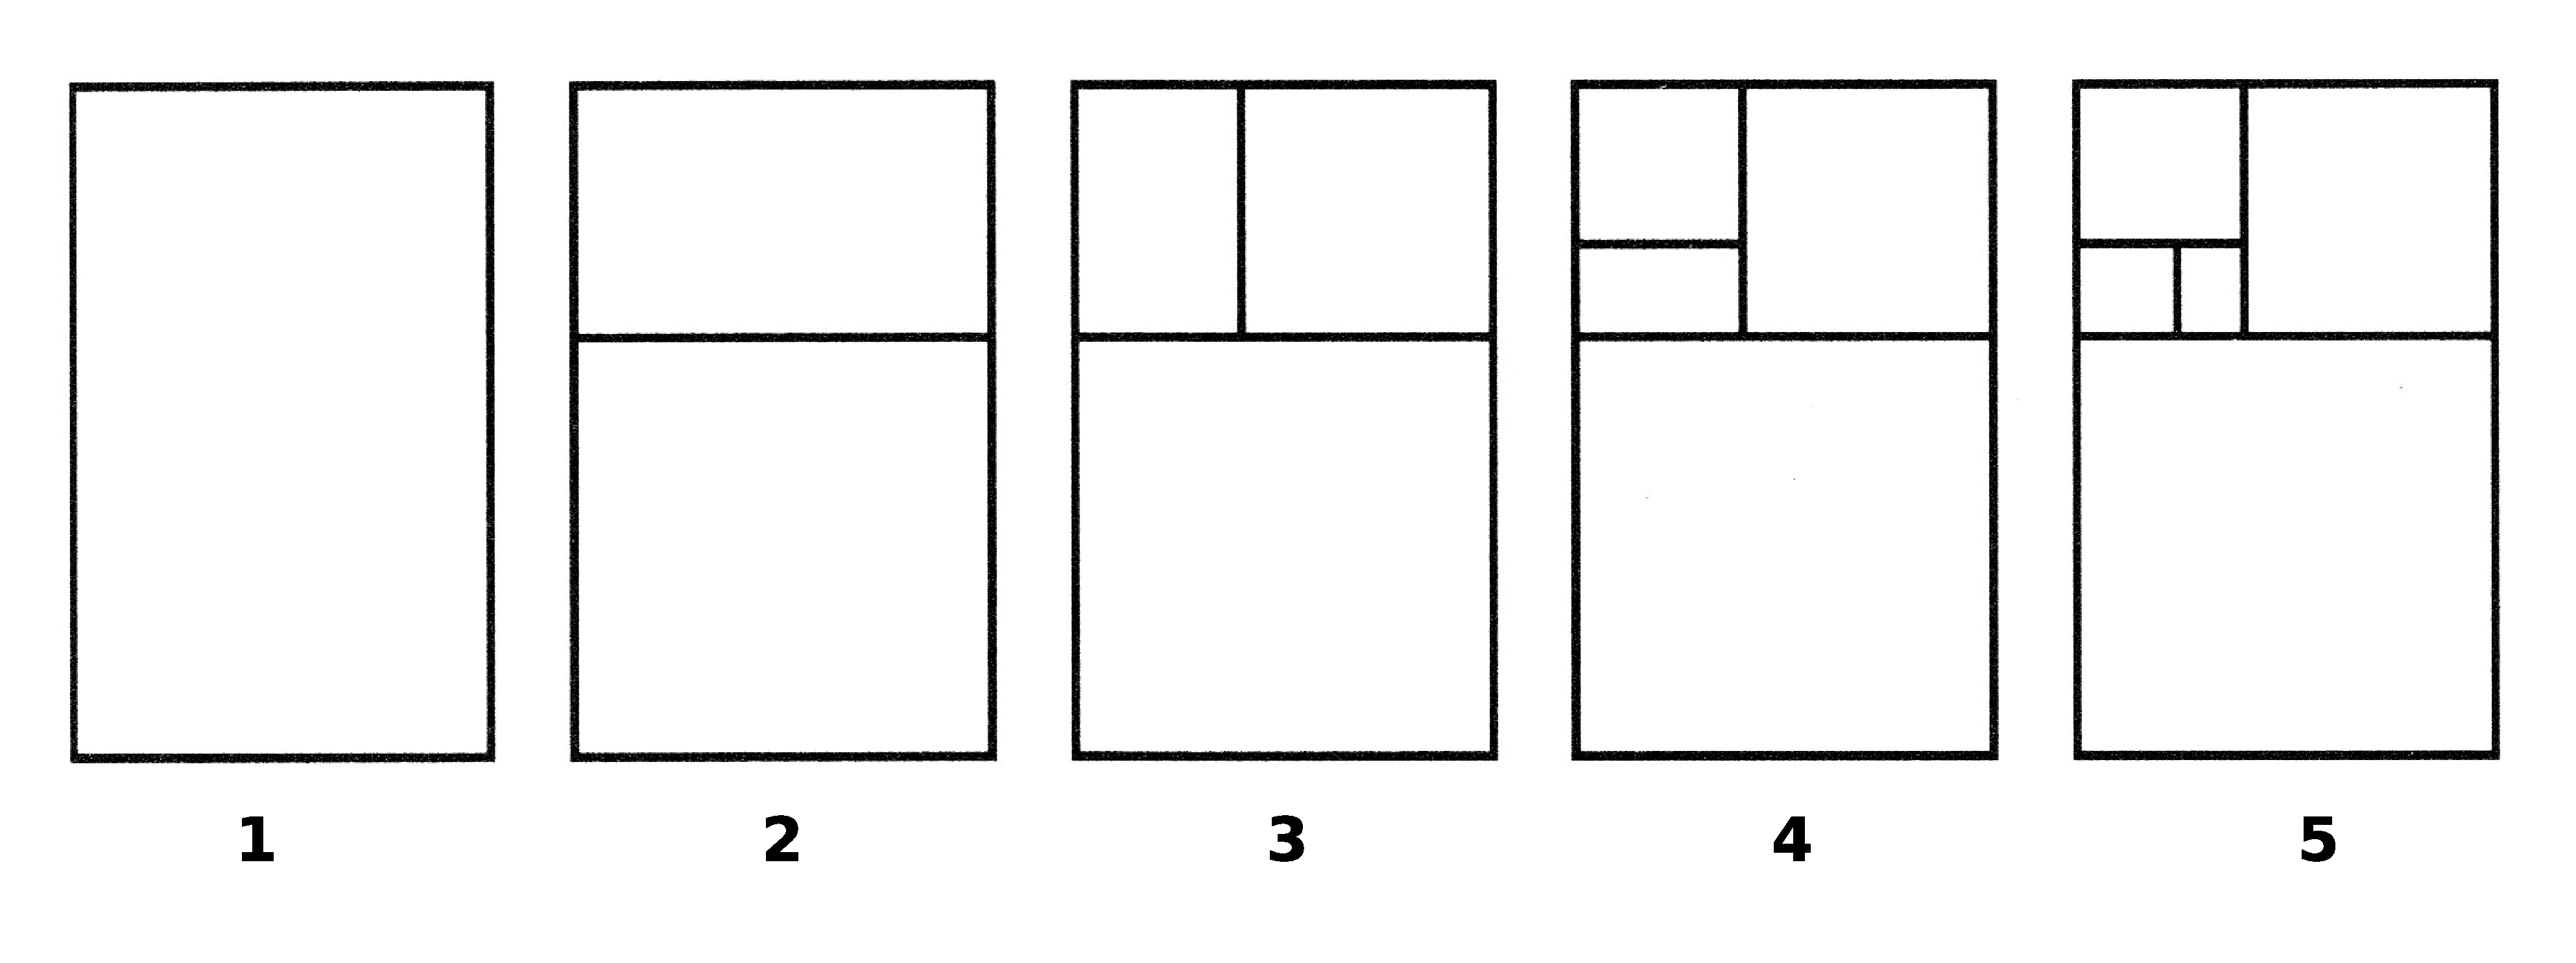
\includegraphics[scale=0.125]{Imatges/figura16-3.pdf}
\end{center}
\caption{Els primers cinc passos en la construcció dels rectangles d'or.}
\label{fig1603}
\end{figure}

Proveu d'identificar accions que us puguin ajudar a aconseguir el vostre objectiu. Preneu, si cal, un tros de paper i dibuixeu un rectangle d'or de 10 cm d'amplada amb un o dos rectangles d'or a dins, com els de la figura~\ref{fig1603}. Per exemple, podríeu definir primer un mètode \textsf{rectangleDaurat:} que dibuixa un rectangle d'or. Després podríeu definir un mètode \textsf{moltsRectanglesDaurats:} que dibuixi diversos rectangles d'or cridant el mètode anterior.

Una altra aproximació és dibuixar un rectangle d'or i traçar una línia dins del rectangle per crear el proper rectangle d'or, i així successivament. No us amoïneu si no us en sortiu a la primera i heu de fer una mica de prova i error, aquest exercici és complicat.

Per ajudar-vos a començar, fixeu-vos en l'\emph{Script}~\ref{scr16-1}, que dibuixa un rectangle d'or. Comenceu convertint aquest \emph{script} en un mètode que té com a paràmetre l'amplada del rectangle.
\begin{script}  Pica dibuixa un rectangle d'or.
\textsf{\upshape
\begin{tabbing}
%\hspace{5mm} \= \kill
$|$ pica longitud amplada $|$\\
pica := Bot nou.\\
amplada := 100.\\
longitud := amplada * ((1 + 5 sqrt) / 2).\\
2 vegadesRepetir:\\
\hspace*{5mm} \= [  pica \= ves: amplada ;\\
\> \> giraEsquerra: 90 ;\\
\> \> ves: longitud ;\\
\> \> giraEsquerra: 90.  ]
\end{tabbing}
}
\label{scr16-1}
\end{script}

\subsection{Una solució d'un-rectangle-per-línia}
\index{rectangles d'or!dibuixar|)}
\index{rectangles d'or!un-rectangle-per-línia|(}
Aquí teniu una solució basada en el fet que només necessiteu dibuixar completament el rectangle més gran. Després d'això podeu dibuixar una sola línia en el lloc adequat per crear el proper rectangle d'or més petit. Aquest procés es mostra a la figura~\ref{fig1604}.
\begin{figure}[h!]
\begin{center}
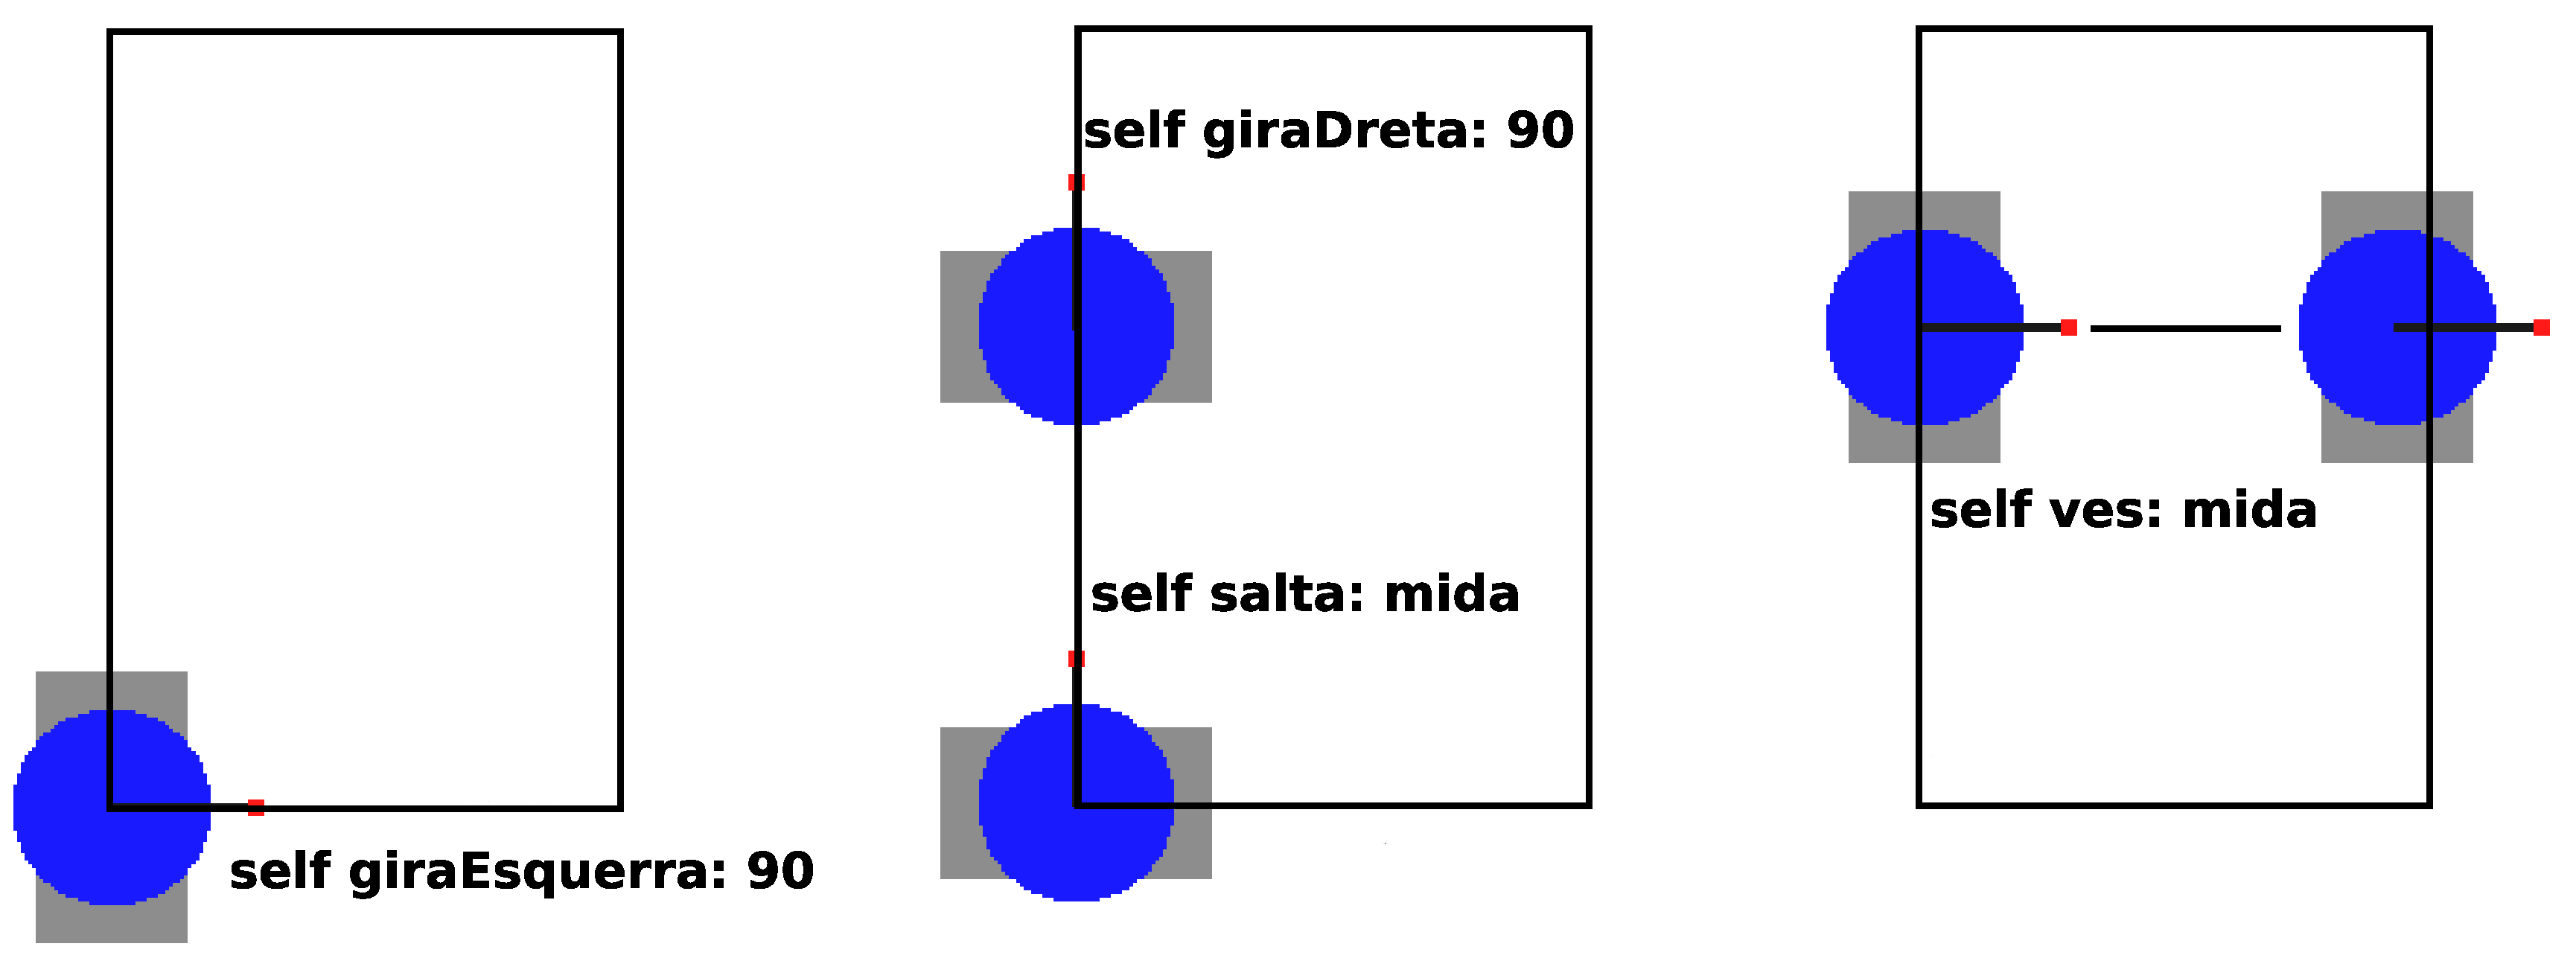
\includegraphics[scale=0.225]{Imatges/figura16-4.pdf}
\end{center}
\caption{Un cop un robot ha dibuixat un rectangle d'or, es col·loca en la posició adequada i dibuixa una línia que talla el rectangle per formar un quadrat i un rectangle d'or més petit.}
\label{fig1604}
\end{figure}

Per tant, per dibuixar diversos rectangles d'or us cal saber com (1) dibuixar un rectangle d'or sencer, (2) dibuixar una línia que defineixi el quadrat dins del rectangle d'or, i (3) calcular l'amplada del proper rectangle d'or. Així, tenim tres tasques:
\begin{itemize}
\item[{\bf 1.}] Definir un mètode que donada una amplada, sap com calcular la llargada corresponent i dibuixa un rectangle d'or, com hem suggerit que féssiu a la secció anterior. Anomenem aquest mètode \textsf{rectangleDaurat: amplada}, on el paràmetre \textsf{amplada} representa l'amplada del rectangle d'or.
\item[{\bf 2.}] Definir un mètode que dibuixa la línia per delimitar el quadrat inclòs dins del rectangle, tal com ho mostra el segon rectangle de la figura ~\ref{fig1603}. Anomenem aquest mètode \textsf{liniaDivisoria: llargada}; primer mou el robot una distància \textsf{llargada} des de la seva posició de partida, i després dibuixa un segment de longitud \textsf{llargada} en la direcció inicial del robot. Fixeu-vos que aquestes dues distàncies són la mateixa ja que són dos costats d'un quadrat.
\item[{\bf 3.}] Un cop els mètodes \textsf{rectangleDaurat:} i \textsf{liniaDivisoria:} han estat definits, us caldrà un mètode que ho combini tot: Hauria de dibuixar un rectangle d'or, i aleshores, repetidament, dibuixar el costat que falta del quadrat per formar el proper rectangle d'or més petit i calcular la mida del proper quadrat, que també és l'amplada del proper rectangle d'or. També necessitareu assegurar-vos que el robot parteix del lloc adequat, i que apunta en la direcció correcta en el moment de dibuixar el proper quadrat.
Anomenem aquest mètode \textsf{rectanglesDaurats: ampleMaxim aNivell: n}, on \textsf{ampleMaxim} representa l'amplada del primer rectangle d'or i \textsf{n} indica el nombre de quadrats que es dibuixaran (de manera que al final hi haurà $n + 1$ retangles d'or).
\end{itemize}

Anem a desenvolupar els tres mètodes.\index{metodes@mètodes!definir per dibuixar rectangles d'or|)}

\vspace*{3mm}
\noindent
{\bf \large El Mètode \textsf{rectangleDaurat: amplada}}
\vspace*{3mm}

El Mètode~\ref{met16-1} no té res d'especial; donada l'amplada d'un rectangle d'or, calcula la llargada i dibuixa el rectangle.\index{rectangleDaurat: mètodes, desenvolupar i exemples de|(}

\begin{metode} Dibuixa un rectangle d'or, donada la seva amplada.
\noindent
\textsf{\upshape
\begin{tabbing}
\hspace{5mm} \= \kill
rectangleDaurat: amplada\\
\> ``Dibuixa un rectangle la llargada del qual és la raó àuria multiplicada per la seva amplada''\\
\\
\> $|$ llargada $|$\\
\> llargada := amplada * (1 + 5 sqrt / 2).\\
\> 2 vegadesRepetir:\\
\> [  self \= ves: amplada ;\\
\> \> giraEsquerra: 90 ;\\
\> \> ves: llargada ;\\
\> \> giraEsquerra: 90.  ]
\end{tabbing}
}
\label{met16-1}
\end{metode}

El mètode \textsf{rectangleDaurat:} comença dibuixant en la direcció actual del robot i dibuixa primer l'amplada del rectangle. Quan acaba, el robot torna al punt de partida apuntant en la direcció original.

\vspace*{3mm}
\noindent
{\bf \large El Mètode \textsf{liniaDivisoria: llargada}}
\vspace*{3mm}

La definició del mètode \textsf{liniaDivisoria:} parteix de la base que el robot és en una cantonada i apuntant cap a l'amplada del rectangle, amb la llargada del rectangle a la seva esquerra. Aquest escenari coincideix amb la situació al final del mètode \textsf{rectangleDaurat:}. La figura~\ref{fig1604} mostra l'acció de \textsf{liniaDivisoria:}, on el robot gira noranta graus a l'esquerra, es desplaça la llargada del rectangle, gira noranta graus a la dreta, i dibuixa el costat que li falta al quadrat per crear el nou rectangle d'or.\index{liniaDivisoria: mètode, desenvolupar per a rectangles daurats|(}

A la situació de la figura~\ref{fig1604}, on el robot és a la base del rectangle d'or i apunta a la dreta (primer dibuix de la figura), acaba dibuixant un segment horitzontal de mida \textsf{llargada} a una distància \textsf{llargada} de la seva posició inicial (tercer dibuix de la figura). Aquesta explicació és de fet més complicada que la definició del mètode.
\begin{metode} Dibuixa una línia que divideix un rectangle d'or en un quadrat i un rectangle d'or més petit.
\noindent
\textsf{\upshape
\begin{tabbing}
\hspace{5mm} \= \kill
liniaDivisoria: llargada\\
\> ``Mou la distància llargada a l'esquerra de la posició inicial,\\
\> i dibuixa un segment de mida llargada en la direcció inicial''\\
\\
\> self \= giraEsquerra: 90 ;\\
\> \> salta: llargada ;\\
\> \> giraDreta: 90 ;\\
\> \> ves: llargada \\
\end{tabbing}
}
\label{met16-2}
\end{metode}
\index{liniaDivisoria: mètode, desenvolupar per a rectangles daurats|)}

\noindent
{\bf \large El Mètode \textsf{rectanglesDaurats: ampleMaxim aNivell: n}}
\vspace*{3mm}

Aquest mètode, Mètode~\ref{met16-3}, és una mica més complicat. Proveu d'entendre'l vosaltres mateixos abans de llegir-ne l'explicació.\index{rectangles d'or!imbricar}
\newpage
\begin{metode}
\noindent
\textsf{\upshape
\begin{tabbing}
\hspace{10mm} \= \hspace{5mm} \= \kill
rectanglesDaurats: ampleMaxim aNivell: n\\
\hspace*{3mm} ``Dibuixa n + 1 rectangles d'or; el més gran té amplada ampleMaxim''\\
(1) \> $|$ ampleActual $|$\\
(2) \> ampleActual := ampleMaxim.\\
(3) \> self rectangleDaurat: ampleActual.\\
(4) \> n vegadesRepetir: [  self liniaDivisoria: ampleActual.\\
(5) \> \> self giraEsquerra: 90.\\
(6) \> \> ampleActual := ampleActual * ((1 + 5 sqrt) / 2 - 1) ]
\end{tabbing}
}
\label{met16-3}
\end{metode}

Aquest mètode genera un grup de rectangles d'or un dins de l'altre el primer dels quals té \textsf{ampleMaxim} com a amplada. Per crear sis rectangles d'or, executeu l'expressió \textsf{Bot nou rectanglesDaurats: 100 aNivell: 5}. Això és el que passa:
\begin{itemize}
\item[$\bullet$] La variable \textsf{ampleActual} representa l'amplada del rectangle actual. També representa la mida del segment del quadrat que queda per dibuixar.
\item[$\bullet$] La línia \textsf{(2)} inicialitza el valor de la variable \textsf{ampleActual} a l'amplada del primer rectangle d'or. Aquesta amplada es dóna com a argument del mètode. Aquesta és l'amplada del primer rectangle d'or.
\item[$\bullet$] La línia \textsf{(3)} dibuixa el primer rectangle d'or, que serveix de base a la resta de rectangles.
\item[$\bullet$] La línia \textsf{(4)} defineix un bucle que repeteix les mateixes accions \textsf{n} vegades. \begin{itemize}
\item[$\bullet$] La línia \textsf{(4)} primer dibuixa la part que falta del quadrat utilitzant el mètode \textsf{liniaDivisoria:}. La mida d'aquest quadrat és l'amplada del rectangle d'or actual. Per tant, el mètode utilitza la variable \textsf{ampleActual} com a argument. Fixeu-vos que utilitzar la variable \textsf{ampleMaxim} no funcionaria per als rectangles petits, ja que el seu valor no canvia dins del cos del bucle.
\item[$\bullet$] La línia \textsf{(5)} posiciona el robot de manera que pugui dibuixar el proper segment. La nostra hipòtesi de partida és que el rectangle sempre es dibuixa amb la seva amplada en la direcció apuntada pel robot. Així, l'expressió \textsf{self giraEsquerra:90} apunta el robot cap a l'amplada del nou rectangle (per exemple, després del darrer dibuix de la figura~\ref{fig1604}, el robot girarà de l'est al nord).
\item[$\bullet$] La darrera línia sorgeix de l'observació que la llargada d'un rectangle d'or és l'amplada del rectangle anterior. Per tant, l'amplada d'un nou rectangle és la diferència entre la llargada i l'amplada del rectangle previ. Expressant-ho matemàticament, tenim
\vspace*{2mm}

\noindent
{\bf novaAmplada = llargadaRectangleActual $-$ ampladaRectangleActual}

\noindent
A partir de la fórmula de la raó àuria, 
\vspace*{2mm}

\noindent
{\bf llargadaRectangleActual = $\frac{1 + \sqrt{5}}{2}$ $\times$ ampladaRectangleActual}
\vspace*{2mm}

\noindent
Per tant,
\vspace*{2mm}

\noindent
{\bf novaAmplada = ampladaRectangleActual $\times$ $\left( \frac{1 + \sqrt{5}}{2} - 1\right)$}
\vspace*{2mm}

\noindent
A Smalltalk escrivim això com: \textsf{ampleActual := ampleActual * ((1 + 5 sqrt) / 2 - 1)}.
\end{itemize}
\end{itemize}

Els problemes de dibuixar un rectangle d'or i dibuixar la línia divisòria són força senzills. La composició de les solucions d'aquests dos problemes per obtenir la solució desitjada requereix parar atenció a les suposicions que fem per tal que cada mètode funcioni correctament, és a dir, el context pel qual ha estat definit.

Potser voleu provar de trobar una altra solució a aquest problema. Podeu utilitzar la mateixa tècnica amb l'Experiment 16-10.\index{rectangles d'or!un-rectangle-per-línia|)}

\begin{center}
\colorbox{black}{\makebox[\textwidth]{  \color{white} {\large {\bfseries Experiment 16-10 (rectangles d'or incrementals)}}}}
\end{center}
\index{rectangles d'or incrementals, Experiment}
\index{Experiments!rectangles d'or incrementals}
\index{rectangleDaurat: mètodes, desenvolupar i exemples de|)}
{\small
\noindent
Heu vist un mètode per dibuixar un conjunt de rectangles d'or \emph{decreixents}. Ara feu un mètode per crear un conjunt de rectangles d'or creixents. Les figures d'aquí sota us ensenyen alguns possibles passos.}
\begin{center}
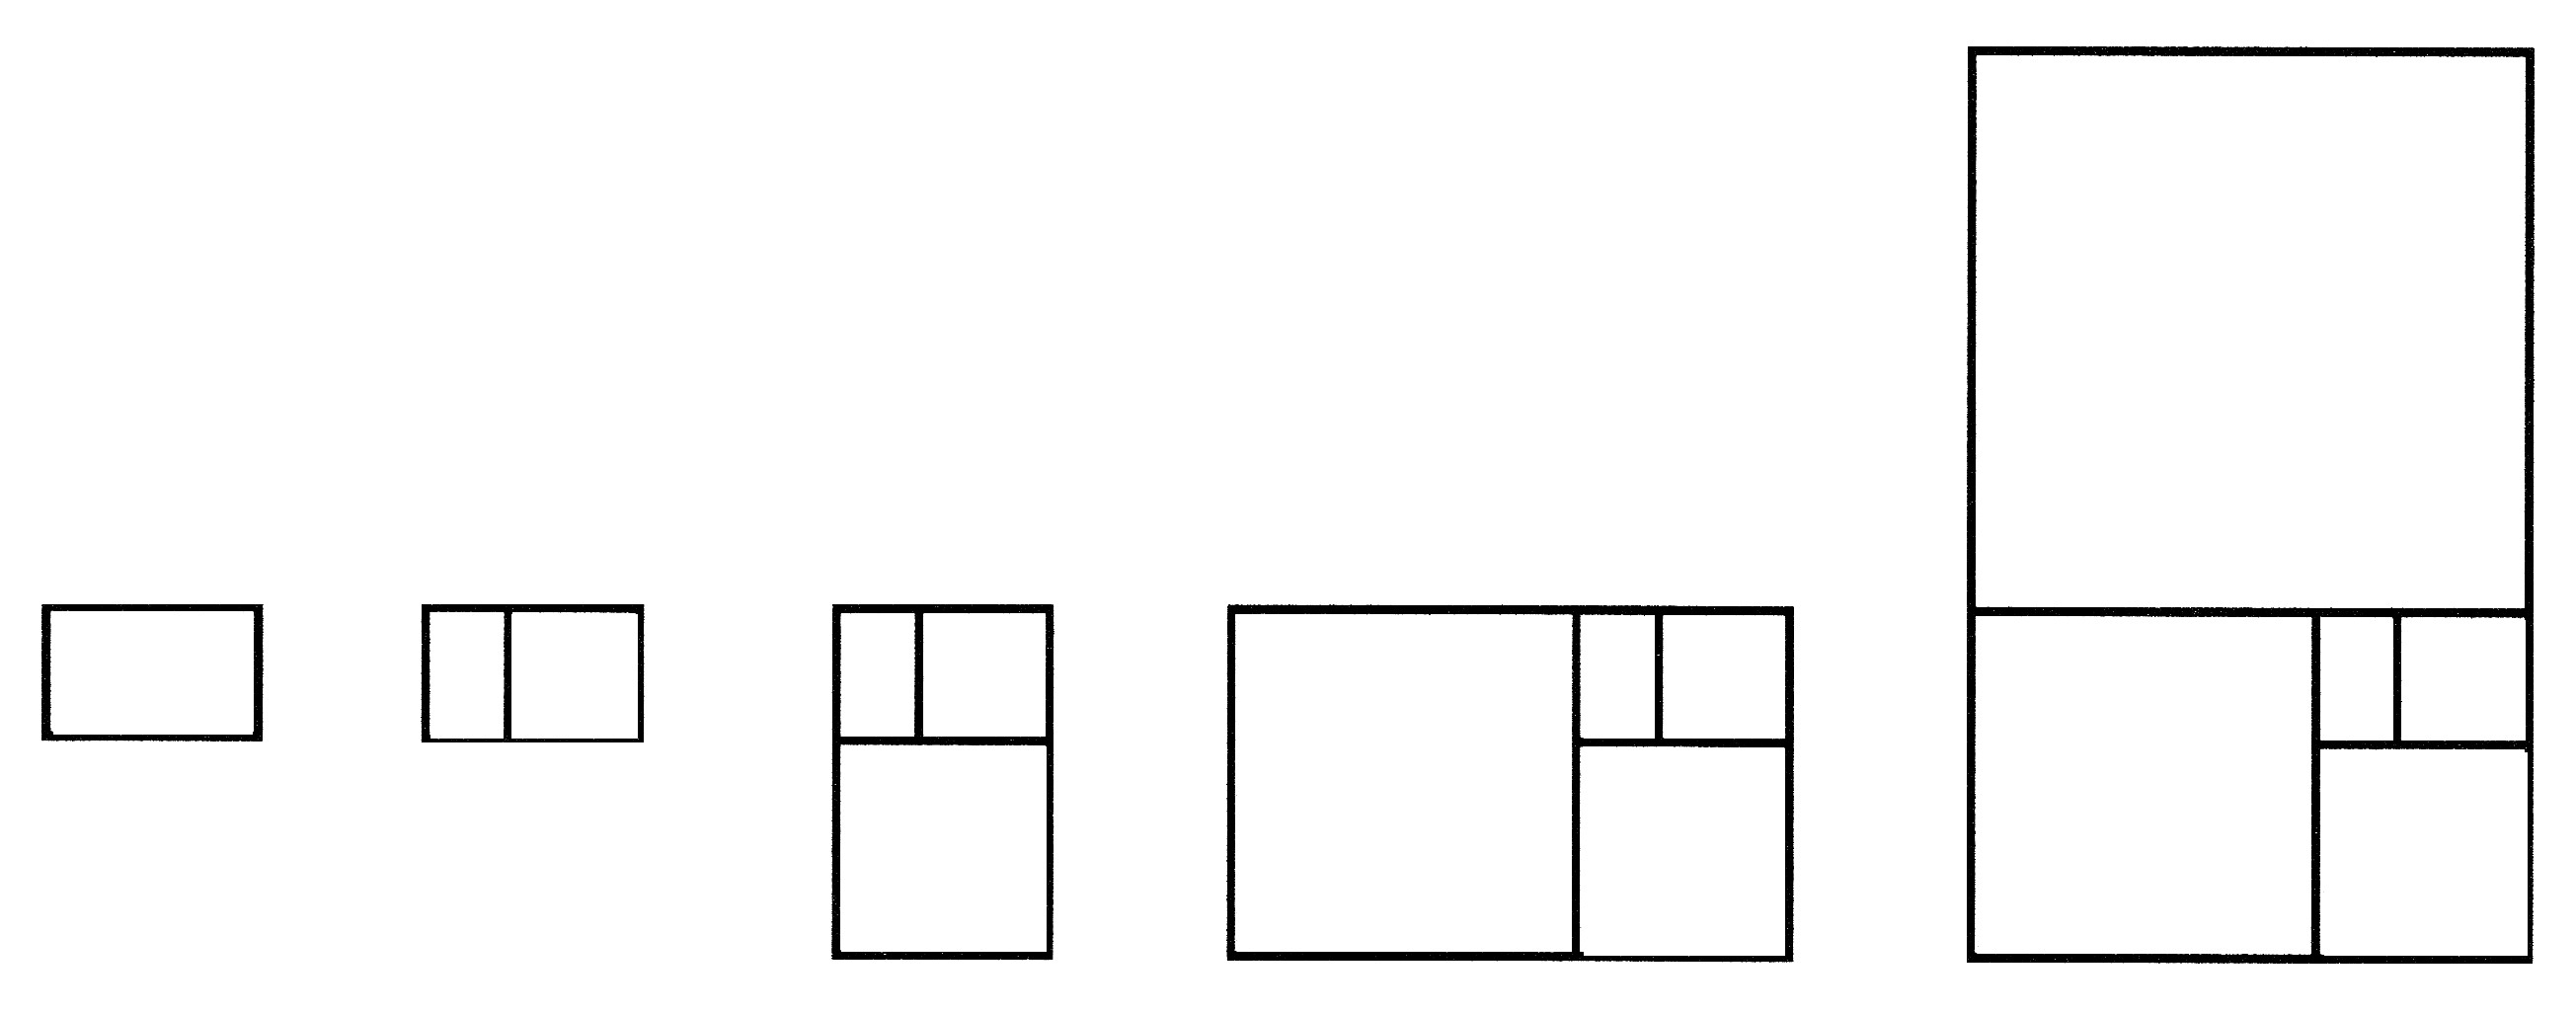
\includegraphics[scale=0.1]{Imatges/figuraE16-10.jpg} 
\end{center}
\noindent
\rule{\textwidth}{3pt}

\section{Enrajolar}
\index{quadrat: mètode!reproduir figures amb|(}
\index{enrajolar quadrats|(}
Ara ens agradaria que intentéssiu reproduir algunes figures utilitzant el mètode \textsf{quadrat:}. Aquests experiments són importants per desenvolupar i entendre la composició de mètodes i la reutilització de les abstraccions que representen. La idea que intentem promoure amb aquests exercicis és fonamental per entendre com es construeixen els programes complexos.

Us donarem algunes pautes: Primer de tot, hi ha diverses maneres d'aproximar-se als problemes. En general, proveu de veure com simplificar-los. Si mireu les tres figures dels tres experiments següents, podeu imaginar-vos que seria força convenient disposar d'un mètode anomenat, diguem, \textsf{filaDeQuadrats:} que pogués dibuixar una fila d'un nombre arbitrari de quadrats. Suposant que tinguéssiu aquesta solució, proveu de donar un esquema de solució per a cada un dels problemes. Després, implementeu el mètode i comproveu si us ha ajudat. Descompondre un problema és difícil, i l'única manera d'aprendre'n és inventant i provant diferents idees, avaluant el resultat, millorant la idea, i provant-ho altre cop.

Com a alternativa, també podeu utilitzar bucles dins d'altres bucles: \index{bucles imbricats, exemples de|(}

\noindent
\textsf{\upshape
\begin{tabbing}
\hspace{5mm} \= \kill
n vegadesRepetir:  [ \\
\> m vegadesRepetir:  [ \dots ] ]\\
\end{tabbing}}

També us suggerim que definiu els vostres mètodes de manera que acabin col·locant el robot al punt de partida. Això fa més senzill compondre els mètodes. Experimenteu amb totes aquestes aproximacions.

\begin{center}
\colorbox{black}{\makebox[\textwidth]{  \color{white} {\large {\bfseries Experiment 16-11 (Una Piràmide Rectangular)}}}}
\end{center}
\index{piràmide rectangular@Una Piràmide Rectangular, Experiment}
\index{Experiments!piràmide rectangular@Una Piràmide Rectangular}
{\small
\noindent
Utilitzant el mètode \textsf{quadrat:}, que dibuixa un quadrat d'una mida determinada, \textsf{filaDeQuadrats:}, que dibuixa una fila de quadrats, i altres mètodes que pugueu definir, dibuixeu la piràmide que veieu aquí a sota.}
\begin{center}
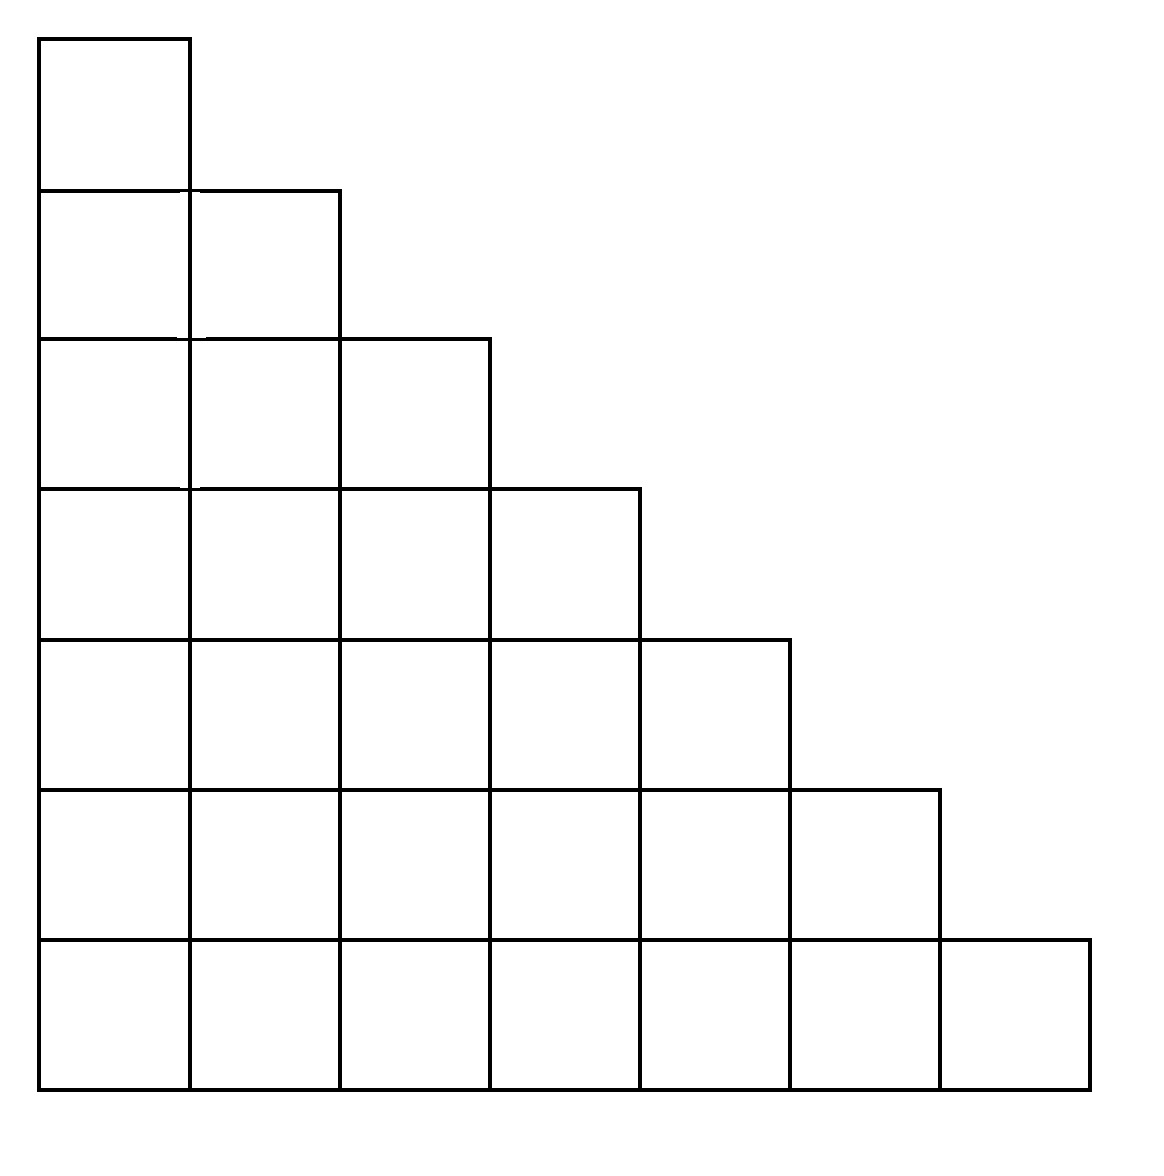
\includegraphics[scale=0.5]{Imatges/figuraE16-11.png} 
\end{center}
\noindent
\rule{\textwidth}{3pt}
\newpage
\begin{center}
\colorbox{black}{\makebox[\textwidth]{  \color{white} {\large {\bfseries Experiment 16-12 (una piràmide triangular)}}}}
\end{center}
\index{piràmide triangular@una piràmide triangular, Experiment}
\index{Experiments!piràmide triangular@una piràmide triangular}
{\small
\noindent
Utilitzant el mètode \textsf{quadrat:}, que dibuixa un quadrat d'una mida determinada, \textsf{filaDeQuadrats:}, que dibuixa una fila de quadrats, i altres mètodes que pugueu definir, dibuixeu la piràmide que veieu aquí a sota.}
\begin{center}
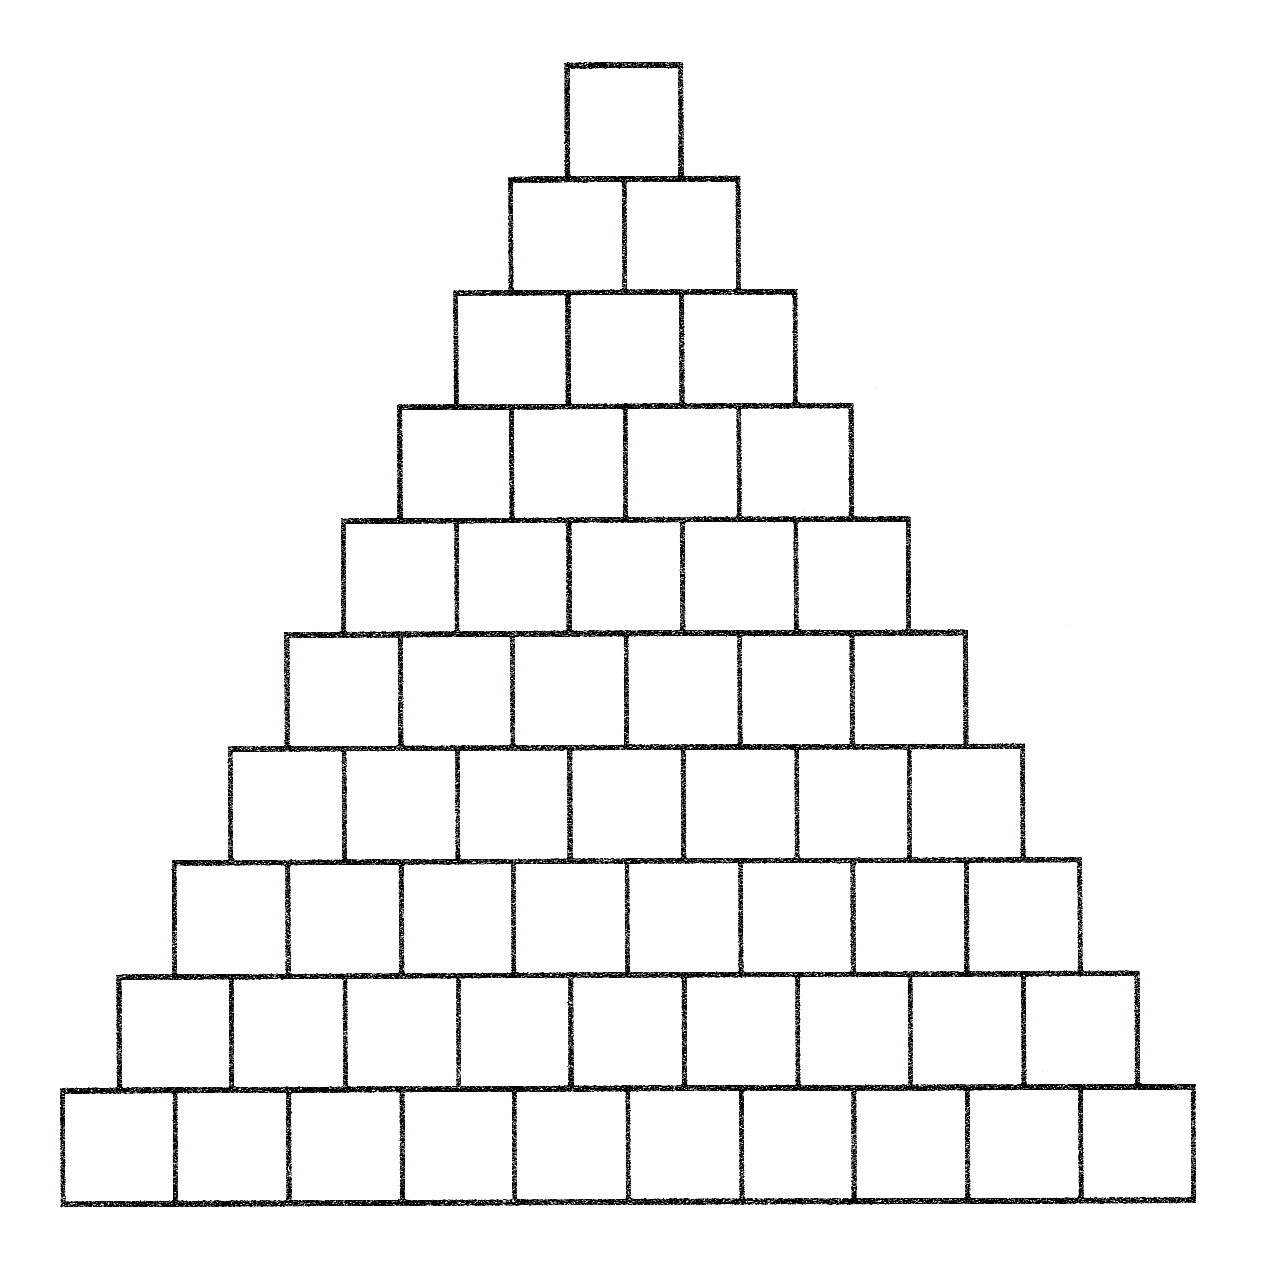
\includegraphics[scale=0.125]{Imatges/figuraE16-12.jpg} 
\end{center}
\noindent
\rule{\textwidth}{3pt}

\begin{center}
\colorbox{black}{\makebox[\textwidth]{  \color{white} {\large {\bfseries Experiment 16-13 (tauler de dames)}}}}
\end{center}
\index{tauler de dames, Experiment}
\index{Experiments!tauler de dames}
{\small
\noindent
Utilitzant el mètode \textsf{quadrat:}, que dibuixa un quadrat d'una mida determinada, \textsf{filaDeQuadrats:}, que dibuixa una fila de quadrats, i altres mètodes que pugueu definir, dibuixeu el tauler que veieu aquí a sota.}
\begin{center}

\includegraphics[scale=0.4]{Imatges/figuraE16-13.png} 
\end{center}
\noindent
\rule{\textwidth}{3pt}

\section{Resum}
\index{enrajolar quadrats|)}
\index{quadrat: mètode!reproduir figures amb|)}
\index{bucles imbricats, exemples de|)}
\index{quadrats centrats, crear|seealso{quadrats}}
\begin{itemize}
\item Per resoldre un problema gran, descomponeu-lo en problemes més petits; aleshores torneu a compondre la solució als problemes més petits per arribar a la solució del problema gran.
\item Pareu atenció al context en què els problemes petits es resolen, ja que caldrà assegurar-vos que aquest context no us passa per alt en el moment de compondre les solucions.
\end{itemize}

\chapter{Cadenes, i eines per entendre programes} 
\label{cap17}

En aquest capítol us presentem un concepte important: la noció de cadena de caràcters\footnote{\emph{Nota del Traductor:} En anglès s'anomenen \emph{Strings}, classe d'Smalltalk que, com ja hem dit, no s'ha traduït. A més, per no utilitzar l'expressió composta ``cadenes de caràcters'' tota l'estona, i seguint els consells de SoftCatalà, les anomenarem ``cadenes'' d'ara en endavant.}. Una cadena és una seqüència de caràcters que podem utilitzar per representar paraules o frases. Una utilització destacada de les cadenes és la interacció amb l'usuari. En propers capítols, aprendreu a utilitzar les cadenes com a eina per entendre estructures més complexes, com ara condicions i bucles condicionals. En aquest capítol us presentarem només les característiques més importants de les cadenes, la informació bàsica que utilitzareu després en propers capítols. També us ensenyarem com utilitzar cadenes per ajudar-vos a entendre l'execució dels programes. Finalment us recomanem que proveu d'utilitzar el depurador com a ajut per a la comprensió dels experiments proposats en aquest capítol.

\section{Cadenes}
\index{cadenes de caràcters!panorama general}
Les cadenes s'utilitzen per representar informació i mostrar-la a l'usuari. Les cadenes estan delimitades per cometes simples (\textsf{'Això és una cadena de caràcters'}), i, com podeu veure, poden contenir espais. Per exemple, la cadena \textsf{'Squeak és interessant'} representa una seqüència de vint-i-un caràcters: S q u e \dots Fixeu-vos que l'espai és també un caràcter. Una cadena pot contenir qualsevol nombre de caràcters, fins i tot zero. Per tant, \textsf{''} és una cadena buida, \textsf{'a'} és una cadena amb un sol caràcter a, i \textsf{'  '} és una cadena amb un sol caràcter espai.
\index{' (cometes simples), utilitzades en cadenes de caràcters} \index{cometes simples ('), utilitzades en cadenes de caràcters}
\noindent
\rule{\textwidth}{2pt}
\noindent
\textbf{Important!} Una cadena és una seqüència de caràcters delimitada per cometes simples. Una cadena representa informació textual, com paraules o frases. Les cadenes es poden utilitzar per mostrar informació a la pantalla.\\
\noindent
\rule{\textwidth}{2pt}

\vspace*{3mm}

Seleccionant una cadena i triant \textbf{escriu-ho} al menú, s'escriu la cadena. Les cadenes tenen associades diversos mètodes, però el més important dins del context d'aquest llibre és el mètode \textsf{,} amb el caràcter coma com a nom. Quan s'envia el missatge \textsf{,} a una cadena com a receptor amb una cadena com a argument, el mètode \textsf{,} retorna una cadena resultat de concatenar el receptor amb l'argument. És a dir, retorna una cadena els caràcters de la qual són els de la primera cadena seguits dels caràcters de la segona cadena.

\noindent
\textsf{\upshape
\begin{tabbing}
\hspace{50mm} \= \kill
'squeak' \> ``el valor d'una cadena és la cadena mateixa''\\
{\itshape -- Escriure el valor retornat: 'squeak'}\\
\\
'a' \> ``el valor d'una cadena és la cadena mateixa''\\
\\
'' \> ``una cadena buida''\\
\\
'squeak' , 'és interessant' \> ``concatenar dues cadenes''\\
{\itshape -- Escriure el valor retornat: 'squeak és interessant'}\\
\\
'squeak' , ' ' , 'és interessant' \> ``concatenar múltiples cadenes''\\
{\itshape -- Escriure el valor retornat: 'squeak és interessant'}\\
\end{tabbing}}

El mètode \textsf{copyReplaceAll:with:} us permet modificar una cadena substituint totes les aparicions d'una subcadena particular per una cadena diferent. A l'exemple de sota, \textsf{'no'} és substituït per \textsf{'realment'}:

\noindent
\textsf{\upshape
\begin{tabbing}
\hspace{50mm} \= \kill
'Squeak no és interessant' copyReplaceAll: 'no' with: 'realment'\\
{\itshape -- Escriure el valor retornat: 'Squeak realment és interessant'}\\
\end{tabbing}}

\section{La comunicació amb l'usuari}
\index{usuari, comunicació amb|(}
\index{PopUp menú, exemple de|(}
\index{pantalla!mostrant informació a la|(}
Squeak ofereix eines per mostrar informació per pantalla i per demanar informació a l'usuari. La classe \textsf{PopUpMenu} permet fer aparèixer un menú i mostrar informació a l'usuari utilitzant cadenes. Per exemple, l'expressió \textsf{PopUpMenu inform: 'squeak és interessant'} fa que aparegui una petita finestra mostrant el missatge \textsf{'squeak és interessant'} que s'espera a que l'usuari premi el botó \textbf{ok}. La classe \textsf{FillInTheBlank} permet demanar dades a l'usuari. Per exemple, l'expressió \textsf{FillInTheBlank request: 'és interessant squeak?'} fa aparèixer una capsa de diàleg amb lloc per introduir text i espera que l'usuari escrigui algun text i premi el botó \textbf{Acceptar} o el botó \textbf{Cancel·lar}. El resultat d'aquesta expressió és una cadena que representa el que ha estat escrit per l'usuari. Podeu especificar també una resposta per defecte de l'usuari utilitzant el missatge \textsf{request:initialAnswer:} com podeu veure a l'\emph{script} següent, i a la figura~\ref{fig1701}. \index{request:initialAnswer: missatge, efecte de}

\noindent
\textsf{\upshape
\begin{tabbing}
\hspace{50mm} \= \kill
(1) PopUpMenu inform: 'squeak és interessant'\\
\\
(2) FillInTheBlank request: 'és interessant squeak?'\\
{\itshape -- Escriure el valor retornat: 'si'}\\
\\
(2) FillInTheBlank request: 'és interessant squeak?' initialAnswer: 'és clar que sí!'\\
{\itshape -- Escriure el valor retornat: 'és clar que sí!'}\\
\end{tabbing}}

\begin{figure}[h!]
\begin{center}
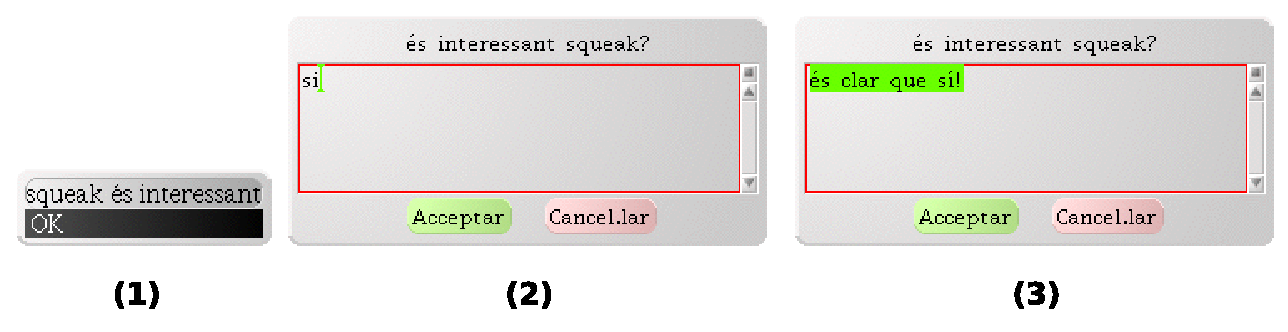
\includegraphics[scale=0.6]{Imatges/figura17-1.pdf}
\end{center}
\caption{Finestres de missatges i d'entrada de dades.}
\label{fig1701}
\index{pantalla!mostrant informació a la|)}
\index{usuari, comunicació amb|)}
\end{figure}

\section{Cadenes i caràcters}
\index{cadenes de caràcters!i caràcters|(}
\index{PopUp menú, exemple de|)}
Una cadena està composta de caràcters. Així com una cadena es col·loca entre cometes simples per deixar clar que és una cadena, els caràcters individuals són prefixats pel signe del dòlar \textsf{\$} per indicar que són caràcters. Per exemple, \textsf{\$a} és el caràcter representant la lletra ``a''. Fixeu-vos que, encara que els caràcters individuals són prefixats per \textsf{\$}, quan s'edita una cadena els caràcters s'escriuren sense el signe del dòlar.

Hi ha diverses maneres d'accedir als caràcters individuals d'una cadena. Per exemple, els mètodes \textsf{first}, \textsf{second} i \textsf{third} retornen el primer, segon o tercer caràcter d'una cadena. El mètode \textsf{size} retorna el nombre de caràcters de la cadena, mentre que el mètode \textsf{at: unNombre} retorna el caràcter present a una posició determinada de la cadena. Podeu substituir el caràcter a una posició específica de la cadena (\textsf{unNombre}) per un altre caràcter utilitzant \textsf{at: unNombre put: unCaracter}. El mètode \textsf{copyUpTo: unCaracter} retorna una cadena composta de tots els caràcters de la cadena receptora des del començament fins el primer caràcter que coincideix amb \textsf{unCaracter}. Aquí teniu alguns exemples: \index{first mètode, exemple de} \index{size mètode, exemple de}

\noindent
\textsf{\upshape
\begin{tabbing}
\hspace{50mm} \= \kill
'squeak és interessant' first\\
{\itshape -- Escriure el valor retornat: \$s}\\
\\
'squeak és interessant' size\\
{\itshape -- Escriure el valor retornat: 21}\\
\\
'squeak' at: 5\\
{\itshape -- Escriure el valor retornat: \$a}\\
\\
'squeak és interessant' at: 11 put: \$f\\
{\itshape -- Escriure el valor retornat: \$f}\\
\\
'squeakésinteressant' copyUpTo: \$i\\
{\itshape -- Escriure el valor retornat: 'squeakés'}\\
\\
'squeak és interessant' copyUpTo: Character space\\
{\itshape -- Escriure el valor retornat: 'squeak'}\\
\end{tabbing}}

Per crear un caràcter sense representació gràfica, com l'espai, el tabulador o el \emph{return}, podeu enviar un missatge a la classe \textsf{Character}. Els missatges \textsf{Character space}, \textsf{Character tab} i \textsf{Character cr} retornen respectivament els caràcters espai, tabulador i \emph{return}. \index{return@\emph{return} caràcters, representar} \index{copyUpTo: mètode, exemple de} \index{espai, caràcter; representar} \index{tab caràcter, representar}

L'\emph{Script}~\ref{scr17-1} mostra com inserir un \emph{return} dins d'una cadena. Fixeu-vos que el mètode \textsf{at:put:} no retorna la cadena modificada, sinó el caràcter inserit. Aquest és un exemple on l'\emph{efecte} d'un missatge i el seu \emph{resultat} són clarament diferents. Escriure el resultat del missatge \textsf{'squeak és interessant' at: 7 put: Character cr} no il·lustra l'efecte del mètode. El que podem fer és escriure la cadena modificada. Per revisar com escriure per pantalla els resultats d'un enviament de missatge, veieu el capítol~\ref{cap5}.
\begin{script}  Inserir un \emph{return} dins una cadena.
\textsf{\upshape
\begin{tabbing}
\hspace{5mm} \= \kill
$|$ laMevaCadena $|$\\
laMevaCadena := 'squeak és interessant'.\\
laMevaCadena at: 7 put: Character cr.\\
laMevaCadena\\
{\itshape -- Escriure el valor retornat: 'squeak}\\
{\itshape és interessant'}\\
\end{tabbing}
}
\label{scr17-1}
\end{script}

Un caràcter pot ser transformat en una cadena enviant-li el missatge \textsf{asString}. A l'\emph{Script}~\ref{scr17-2}, es concatenen tres cadenes. La del mig és la cadena \textsf{'a'} creada per l'enviament de missatge \textsf{\$a asString}.\index{asString missatge, exemple de}
\begin{script}  Un caràcter es transforma en una cadena, que és concatenada amb altres cadenes.
\textsf{\upshape
\begin{tabbing}
\hspace{5mm} \= \kill
'sque', \$a asString, 'k'\\
{\itshape -- Escriure el valor retornat: 'squeak'}\\
\end{tabbing}
}
\label{scr17-2}
\end{script}

\section{Cadenes i nombres}
\index{cadenes de caràcters!i caràcters|)}
\index{nombres i cadenes, panorama general}
\index{cadenes de caràcters!i nombres}
Una cadena pot representar un nombre. Per exemple, la \emph{cadena} '10' és una representació textual del \emph{nombre} 10. Tot i així, una cadena no és un nombre. Una cadena no sap com realitzar cap operació matemàtica, i un nombre no sap com comportar-se com una cadena. Per exemple, no podem concatenar dos nombres o sumar dues cadenes. Tot i així, un nombre sap com generar una cadena que \emph{el representa}, utilitzant el mètode \textsf{asString}. A més, una cadena sap com convertir la representació d'un nombre en un nombre amb el mètode \textsf{asNumber}.

Així doncs, hi ha una diferència entre el nombre \textsf{10} i la cadena \textsf{'10'}. El nombre \textsf{10} representa la quantitat matemàtica 10, mentre la cadena \textsf{'10'} és la representació textual del nombre 10 que consisteix en els dos caràcters 1 i 0. La cadena \textsf{'10'} es compon dels dos caràcters \textsf{\$1} i \textsf{\$0}, i la cadena \textsf{'12'} es compon dels dos caràcters \textsf{\$1} i \textsf{\$2}. Aquí teniu algunes il·lustracions d'operacions amb cadenes i nombres:

\noindent
\textsf{\upshape
\begin{tabbing}
\hspace{50mm} \= \kill
10 , 12\\
{\itshape $\rightarrow$ error! un nombre no coneix el missatge ,}\\
\\
'10' , '12'\\
{\itshape -- Escriure el valor retornat: '1012'}\\
\\
10 asString\\
{\itshape -- Escriure el valor retornat: '10'}\\
\\
10 asString , 12 asString\\
{\itshape -- Escriure el valor retornat: '1012'}\\
\\
'10' asNumber\\
{\itshape -- Escriure el valor retornat: 10}\\
\end{tabbing}}

\noindent
\rule{\textwidth}{2pt}
\noindent
\textbf{Nota} Una cadena (\emph{string}) pot representar un nombre, però aquesta cadena no és un nombre. Per exemple, la cadena \textsf{'79'} es compon dels dos caràcters \textsf{\$7} i \textsf{\$9}. Per aconseguir la cadena que representa un nombre, cal enviar el missatge \textsf{asString} al nombre.\\
\noindent
\rule{\textwidth}{2pt}

\section{Utilitzar el \emph{Transcript}}
\index{execució de programes, utiltzar el \emph{Transcript} per a la|(}
\index{Transcript@\emph{Transcript}, eina!utilitzar el|(}
Squeak us ofereix diverses eines molt potents per entendre l'execució dels programes, com per exemple el depurador que ja vam veure al capítol~\ref{cap15}. Una altra eina s'anomena el \emph{Transcript}\footnote{\emph{Nota del Traductor:} Igual que ens ha passat amb \emph{script}, deixarem \emph{Transcript} en anglès, escrivint-lo en cursiva per deixar clar que és un anglicisme.}, i pot mostrar informació textual amb cadenes de caràcters. Per obrir una finestra de \emph{Transcript}, arrossegueu la icona disponible en una de les solapes a l'entorn, o trieu l'opció \textbf{transcript} del menú \textbf{obrir \dots}. Això obre una finestra com la que veieu a la figura\ref{fig1702}.
\begin{figure}[h!]
\begin{center}
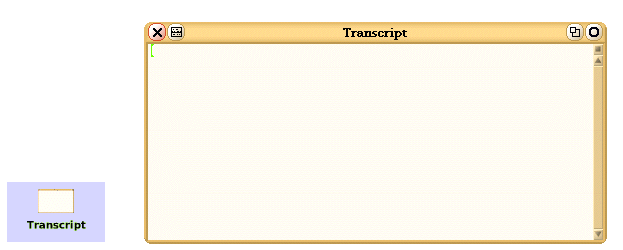
\includegraphics[scale=2.5]{Imatges/figura17-2.png}
\end{center}
\caption{Per obrir una finestra amb un \emph{Transcript} arrossegueu i deixeu dins l'entorn la icona que podeu trobar en una solapa.}
\label{fig1702}
\end{figure}

Hi ha dos missatges per mostrar informació en un \emph{Transcript}: \textsf{show:} i \textsf{cr}. El missatge \textsf{show: unaCadena} escriu la cadena a la finestra, i el missatge \textsf{cr} insereix una línia nova. Veieu la figura~\ref{fig1703}.
\begin{figure}[h!]
\begin{center}
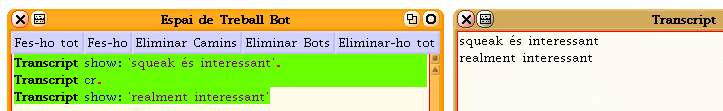
\includegraphics[scale=2.5]{Imatges/figura17-3.png}
\end{center}
\caption{Escriure dins d'un \emph{Transcript}.}
\label{fig1703}
\end{figure}

L'\emph{Script}~\ref{scr17-3} dóna alguns exemples mostrant informació en un \emph{Transcript}.
\begin{script}  Mostrar informació en una finestra de \emph{Transcript}
\textsf{\upshape
\begin{tabbing}
\hspace{5mm} \= \kill
Transcript show: 'squeak és interessant'.\\
Transcript cr.\\
Transcript show: 'realment interessant'.\\
\end{tabbing}
}
\label{scr17-3}
\end{script}

Fixeu-vos que una finestra amb un \emph{Transcript} només pot mostrar cadenes. Per tant, si voleu escriure un nombre, haureu d'obtenir la cadena que el representi amb el mètode \textsf{asString}, Això ho il·lustrem a l'\emph{Script}~\ref{scr17-4}. \index{nombres i cadenes, panorama general} \index{cadenes de caràcters!i nombres}

\begin{script} Un nombre es transforma en una cadena abans de poder ser escrit.
\textsf{\upshape
\begin{tabbing}
\hspace{5mm} \= \kill
Transcript show: '21 + 21 és: ' , 42 asString ; cr\\
\end{tabbing}
}
\label{scr17-4}
\end{script}

\section{Generar i comprendre una traça}
\index{traces!generar|(}
\index{Transcript@\emph{Transcript}, eina!utilitzar el|)}
\index{execució de programes, utiltzar el \emph{Transcript} per a la|)}
\index{Transcript@\emph{Transcript}, eina!generar traces de programes amb|(}
\index{:= (expressió d'assignació)!utilitzar per fer traces}
\index{moviments de robot, seguiment dins dels \emph{scripts}}
\index{escala!dibuixar amb esglaons|(}
\index{esglaons!dibuixar una escala amb|(}
Ara ens agradaria ensenyar-vos com podeu utilitzar la classe \textsf{Transcript} per generar la traça d'un programa. Una traça és una col·lecció d'indicadors del que està passant generats per un programa. Per exemple, podria ser que volguéssiu
seguir els moviments d'un robot en un \emph{script} fent que l'\emph{script} escrigués \textsf{'Estic girant a la dreta'} cada cop que el robot giri a la dreta. Per generar una traça, simplement cal que introduïu una o més expressions dins del vostre \emph{script} que no canviïn l'execució original del programa però que, per exemple, mostrin informació en un \emph{Transcript}. Comencem amb l'\emph{Script}~\ref{scr17-5}, que dibuixa una escala amb esglaons de longitud creixent.
\begin{script} Una escala amb esglaons de longitud creixent.
\textsf{\upshape
\begin{tabbing}
\hspace{5mm} \= \kill
$|$ pica  longitudEsglao $|$\\
pica := Bot nou.\\
longitudEsglao := 10.\\
10 vegadesRepetir:\\
\> [ pica ves: longitudEsglao.\\
\> pica giraEsquerra: 90.\\
\> pica ves: 5.\\
\> pica giraDreta: 90.\\
\> longitudEsglao := longitudEsglao + 10.  ]
\end{tabbing}
}
\label{scr17-5}
\end{script}

La primera traça senzilla que podem generar ens diu quan el programa està tot just a punt d'entrar al bucle \textsf{vegadesRepetir:}, i quan ha sortit del bucle. Això es pot veure a l'\emph{Script}~\ref{scr17-6}.
\begin{script} L'escala amb una traça senzilla.
\textsf{\upshape
\begin{tabbing}
\hspace{5mm} \= \kill
$|$ pica  longitudEsglao $|$\\
pica := Bot nou.\\
longitudEsglao := 10.\\
{\bfseries Transcript show: 'Abans del bucle' ; cr.}\\ 
10 vegadesRepetir:\\
\> [ pica ves: longitudEsglao.\\
\> pica giraEsquerra: 90.\\
\> pica ves: 5.\\
\> pica giraDreta: 90.\\
\> longitudEsglao := longitudEsglao + 10.  ]\\
{\bfseries Transcript show: 'Després del bucle' ; cr.}\\ 
\end{tabbing}
}
\label{scr17-6}
\end{script}

 \begin{center}
\colorbox{black}{\makebox[\textwidth]{  \color{white} {\large {\bfseries Experiment 17-1 (posar una traça dins del bucle)}}}}
\end{center}
\index{posar una traça dins del bucle, Experiment}
\index{Experiments!posar una traça dins del bucle}
{\small
\noindent
Modifiqueu l'\emph{Script}~\ref{scr17-6} introduint l'expressió \textsf{Transcript show: 'dins del bucle' ; cr.} dins del bucle. El vostre \emph{transcript} hauria d'escriure \textsf{'dins del bucle'} deu vegades, una vegada cada iteració. També podeu inserir l'expressió \textsf{self halt} per permetre obrir el depurador. Aneu amb compte, però, sinó acabareu amb deu depuradors!.}\\
\noindent
\rule{\textwidth}{3pt}
\vspace*{2mm}

Ara utilitzarem la mateixa tècnica per generar una traça una mica més sofisticada. Per exemple, estaria bé veure com canvia el valor de la variable \textsf{longitudEsglao} mentre s'executa el programa. L'\emph{Script}~\ref{scr17-7} conté una expressió nova que escriu el valor de la variable \textsf{longitudEsglao} al començament del bucle cada cop que és executat. Els resultats els podeu veure a la figura~\ref{fig1704}.
\begin{figure}[h!]
\begin{center}
\includegraphics[scale=2.5]{Imatges/figura17-4.png}
\end{center}
\caption{Afegir una traça a un \emph{script}.}
\label{fig1704}
\index{scripts@\emph{scripts}|seealso{Experiments}}
\index{scripts@\emph{scripts}!afegir traces als}
\end{figure}

\begin{script} L'escala amb una traça més sofisticada.
\textsf{\upshape
\begin{tabbing}
\hspace{5mm} \= \kill
$|$ pica  longitudEsglao $|$\\
pica := Bot nou.\\
longitudEsglao := 10.\\
10 vegadesRepetir:\\
\> [  {\bfseries Transcript show: '\textgreater\textgreater\hspace*{1mm}' , longitudEsglao asString ; cr.}\\ 
\> pica ves: longitudEsglao.\\
\> pica giraEsquerra: 90.\\
\> pica ves: 5.\\
\> pica giraDreta: 90.\\
\> longitudEsglao := longitudEsglao + 10.  ]
\end{tabbing}
}
\label{scr17-7}
\end{script}

Afegir una traça a una assignació és sovint útil, ja que revela un comportament important del programa. Per exemple, a l'\emph{Script}~\ref{scr17-8}, l'expressió \textsf{Transcript show: 'Després := ' , longitudEsglao asString ; cr.} s'ha afegit després de la instrucció d'assignació que és la darrera expressió del bucle. La traça, que teniu tot seguit de l'\emph{script}, escriu el valor de la variable \textsf{longitudEsglao} al començament i al final del bucle. Aquests dos valors haurien de ser el mateix, i, de fet, ho són, com veieu a la traça.\index{:= (expressió d'assignació)!utilitzar en traces} \index{escala!dibuixar amb esglaons|)} \index{traces!generar|)}\index{Transcript@\emph{Transcript}, eina!generar traces de programes amb|)} \index{esglaons!dibuixar una escala amb|)}
\newpage
\begin{script} L'escala amb una traça després d'una assignació.
\textsf{\upshape
\begin{tabbing}
\hspace{5mm} \= \kill
$|$ pica  longitudEsglao $|$\\
pica := Bot nou.\\
longitudEsglao := 10.\\
10 vegadesRepetir:\\
\> [  {\bfseries Transcript show: 'longitudEsglao: ' , longitudEsglao asString ; cr.}\\ 
\> pica ves: longitudEsglao.\\
\> pica giraEsquerra: 90.\\
\> pica ves: 5.\\
\> pica giraDreta: 90.\\
\> longitudEsglao := longitudEsglao + 10.\\
\> {\bfseries Transcript show: 'longitudEsglao després de := ' , longitudEsglao asString ; cr.}  ]\\ 
\end{tabbing}
}
\label{scr17-8}
\end{script}

\noindent
I aquí teniu la traça:
\noindent
\textsf{\upshape
\begin{tabbing}
\hspace{50mm} \= \kill
longitudEsglao:  10\\
longitudEsglao després de :=  20\\
longitudEsglao:  20\\
longitudEsglao després de :=  30\\
longitudEsglao:  30\\
longitudEsglao després de :=  40\\
longitudEsglao:  40\\
longitudEsglao després de :=  50\\
longitudEsglao:  50\\
longitudEsglao després de :=  60\\
longitudEsglao:  60\\
longitudEsglao després de :=  70\\
longitudEsglao:  70\\
longitudEsglao després de :=  80\\
longitudEsglao:  80\\
longitudEsglao després de :=  90\\
longitudEsglao:  90\\
longitudEsglao després de :=  100\\
longitudEsglao:  100\\
longitudEsglao després de :=  110\\
\end{tabbing}}

\section{Resum}

\begin{itemize}
\item Una cadena és una seqüència de caràcters delimitada per cometes simples: \textsf{'Això és una cadena'}. Una cadena representa informació textual com paraules o frases i es pot utilitzar per mostrar informació a la pantalla. Per exemple: \textsf{'squeak és interessant'} és una cadena de 21 caràcters.
\item Un caràcter és una lletra prefixada amb el signe del dòlar \$. Així, \textsf{\$a} representa el caràcter \textsf{a}.
\item Una cadena pot representar un nombre, però aquesta cadena no és un nombre. Per exemple, la cadena \textsf{'79'} es compon dels dos caràcters \textsf{\$7} i \textsf{\$9}. Per aconseguir la cadena que representa un nombre, cal enviar el missatge \textsf{asString} al nombre.
\item Una finestra de \textsf{Transcript} és una petita finestra que s'utilitza per mostrar missatges. El missatge \textsf{show: unaCadena} escriu el valor de l'argument \textsf{unaCadena}, que ha de ser una cadena, a una finestra de \emph{transcript}. El missatge \textsf{cr} insereix una línia nova a una finestra de \emph{transcript}. 
\end{itemize}

